\documentclass[letterpaper,10pt]{book}
% Change to 10 pt
\usepackage{pdfpages}
\usepackage{morewrites}			% to counteract the no write space problem
\setcounter{tocdepth}{5}

\usepackage[framemethod=TikZ]{mdframed}

\usepackage{fancyhdr}

\usepackage{paralist}
\usepackage{amsmath}
\usepackage{amsfonts}
\usepackage{amssymb}
\usepackage{graphicx}

\usepackage{datetime}
%\usepackage{ulem}

%\usepackage[nottoc]{toobibind}

\usepackage[inline]{enumitem}

% Outer margin at 2.50 is exactly correct to fit the ``corruption alert'' tables
\usepackage[inner=1.0in, outer=2.50in, top=2.54cm,bottom=2.54cm, marginparwidth=2.25in]{geometry}

\usepackage{marginnote}
\usepackage{longtable}
\usepackage{booktabs}
\usepackage{xcolor}

\usepackage{soul}

\usepackage{marginnote}
\usepackage{imakeidx} 
\usepackage[
	backref=true,
	style=numeric,
%	citestyle=numeric,
	backend=bibtex
	]{biblatex}
\usepackage[driverfallback=hypertex,colorlinks=True]{hyperref}
\usepackage{cleveref}

\makeindex[name=scripture,columnsep=20pt, columnseprule=True,columns=3, title=Scripture References]
\makeindex[name=speaker,columnsep=20pt, columnseprule=True,,columns=2, title=Sermon Creator]
\makeindex[name=series,columnsep=20pt, columnseprule=True,,columns=2, title=Sermon Series]
\makeindex[name=date,columnsep=20pt, columnseprule=True,columns=2, title=Sermon Date]

\makeindex[name=event,columnsep=20pt, columnseprule=True,columns=2, title=Event]

\makeindex[name=topic,columnsep=20pt, columnseprule=True,columns=2, title=Topic]
\makeindex[name=AWIP,columnsep=20pt, columnseprule=True,columns=3, title=All Words in Passage]
\makeindex[name=NWIV,columnsep=20pt, columnseprule=True,columns=3, title=Number of Words in Verse]
\makeindex[name=PNIP,columnsep=20pt, columnseprule=True,columns=3, title=Proper Names in Passage]
\makeindex[name=PEIP,columnsep=20pt, columnseprule=True,columns=2, title=Prophetic Events in Passage]


\makeindex[name=TWPAQ,columnsep=20pt, columnseprule=True,columns=1, title=13-Word Phrases and Quotes]
\makeindex[name=PFTTIS,columnsep=20pt, columnseprule=False,columns=3, title=Phrases found 13 times in scripture]
\makeindex[name=WFTTIS,columnsep=20pt, columnseprule=False,columns=3, title=Words found 13 times in scripture]
\makeindex[name=WFITV,columnsep=20pt, columnseprule=False,columns=3, title=Words found in exactly 13 verses]
\makeindex[name=EVENTS,columnsep=20pt, columnseprule=False,columns=2, title=Sermon Log by Place]
\makeindex[name=QUESTIONS,columnsep=20pt, columnseprule=False,columns=2, title=Bible Questions]

\makeindex[name=DOCTRINES,columnsep=20pt, columnseprule=False,columns=2, title=Doctrines]

\makeindex[name=SONGS,columnsep=20pt, columnseprule=False,columns=1, title=Songs]
\makeindex[name=LOCATION,columnsep=20pt, columnseprule=False,columns= 2, title=Location]
\makeindex[name=FACEBOOK,columnsep=20pt, columnseprule=False,columns=2, title=Facebook]

\makeindex[name=DEVOTIONAL,columnsep=20pt, columnseprule=False,columns=1, title=Devotionals]

\pagestyle{fancy}
\fancyhf{}
\fancyhead[LE,RO]{\today}
\fancyhead[RE,LO]{Notes, Outlines, Comments}
\fancyhead[CE,CO]{-page \thepage  - }

\fancyfoot[CO,CE]{\leftmark}
%\fancyfoot[LE,RO]{CSCE 692, HW1}

\title{DBR\\
Daily \\ Reads}
\author{Keith Anthony \\
\today }
%\title

%+/ffffff +   \pagenumbering{gobble}

\bibliography{Bibliographies/All20220108}

%%%%% TWEAKS:
%%% - distance from fcolorbox frame to text
\setlength{\fboxsep}{1.0pt}

\usepackage[utf8]{inputenc}
\usepackage{tikz}

%%%%%%%%%%%%%%%%%%%%%%%%%%%%%%%%%%%%%%%%%%%%%%%%%%%%%%%%%%%%%%%%%%%%%%%%%%%%%%%%

\begin{document}

\begin{titlepage}

% Set the text of the page to right-aligned until \end{flushright}
\begin{flushright}
\rightskip=-2.5cm

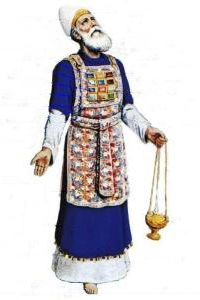
\includegraphics[width=50mm,scale=1.5]{Melchisedec.jpg}
\vspace{0.4in}

% Create a title for the document and write it in bold font
\LARGE{\textbf{\date}}
\linebreak

\vspace{0.5in}


\begin{flushleft}
\LARGE{Psalms 76-100 (Volume IV)\\}\vspace{0.25in}
\LARGE{Notes, Outlines, Comments}
\end{flushleft}

% write in large letters
%\large{Free webservices and apps}

% Skip some space
\vspace{0.6in}

%\large{Documentation}
% Skip some space

\bigskip

\normalsize{Xenia, Oh.\\}
\normalsize{updated: \today}

% Skip some space
\vspace{1.3in}

\end{flushright}
% End the title page
\end{titlepage}

%\titlehttps://www.overleaf.com/project/60d732302fc633866943c9d2JE

\newpage 

\tableofcontents\hypertarget{TOC}{}
\listoffigures
\listoftables

\hyphenation{A-bim-e-lech bre-thren E-phra-im  Gib-e-o-nites Jer-u-sa-lem through-out Phil-i-stines The-o-phil-us Am-a-le-kites ven-geance Mesh-el-e-mi-ah onan-ism Phar-a-oh Py-thon thoughts grev-ous-ness Hach-a-liah adul-ter-er Shad-rach}

%\fcolorbox{black}{bone}{TEXT}
%%%%%%%%%%%%%%%%% EXTRA COLORS
%%%%%%%%%%%%%%%%% EXTRA COLORS
%%%%%%%%%%%%%%%%% EXTRA COLORS
\definecolor{champagne}{rgb}{0.97,0.91,0.81}
\definecolor{bone}{rgb}{0.89,0.85,0.79}

\definecolor{ForestGreen}{rgb}{0.00,0.29,0.098}
\definecolor{GIVING}{cmyk}{1,0.0,0.72,.1}

\definecolor{MLPE}{cmyk}{1,1,0,.45}
\definecolor{SOCCER}{cmyk}{.77, 0, .42, .49}
\definecolor{PAYBILL}{cmyk}{0,0.83,0.76,0.07}
\definecolor{SERMON}{cmyk}{.14,.9,0,.30} % aka seance \href{http://www.flatuicolorpicker.com/purple-cmyk-color-model/}{seance}
\definecolor{BIBLE}{cmyk}{0,.17,.74,.17}
\definecolor{WORKBLUE}{cmyk}{1, .5, 0, .6}
\definecolor{myOrange}{cmyk}{0, .4, .98, .03}
\definecolor{myTan}{cmyk}{0.0,.07,.17,.10}
\definecolor{myRed}{cmyk}{0,1,1,0}
\definecolor{myWhite}{cmyk}{0,0,0,0}
\definecolor{BLUESoD}{cmyk}{.97,.84,0,.04}
\definecolor{WHITE}{cmyk}{0,0,0,0}
\definecolor{OLDGOLD}{cmyk}{0.05,0.3,1.00,0}
\definecolor{CASTLETON}{cmyk}{1,0,0.31,0.66}
\definecolor{cadmiumgreen}{rgb}{0.0, 0.42, 0.24}
\definecolor{jungle}{rgb}{0.203,0.4882,0.1718}
\definecolor{MYGOLD}{rgb}{1,.84,0}

\definecolor{MYLIGHTGRAY}{rgb}{.85,.85,.85}

\definecolor{codegreen}{rgb}{0,0.6,0}
\definecolor{codegray}{rgb}{0.5,0.5,0.5}
\definecolor{codepurple}{rgb}{0.58,0,0.82}
\definecolor{backcolour}{rgb}{0.95,0.95,0.92}



\mdfdefinestyle{MyFrame}{%
    linecolor=blue,
    outerlinewidth=2pt,
    roundcorner=5pt,
    innertopmargin=\baselineskip,
    innerbottommargin=\baselineskip,
    innerrightmargin=10pt,
    innerleftmargin=10pt,
    backgroundcolor=gray!25!white}


\mdfdefinestyle{MyFrame2}{%
    linecolor=black,
    outerlinewidth=2pt,
    roundcorner=5pt,
    innertopmargin=\baselineskip,
    innerbottommargin=\baselineskip,
    innerrightmargin=10pt,
    innerleftmargin=10pt,
    backgroundcolor=yellow!25!white}



%\input{PFTTIS}
%\input{WFTTIS}
%\input{WFITV}

%
%\newpage
%\begin{figure}
%\begin{center}
%\includegraphics[scale=.7, angle=0]{05OT-Deuteronomy/References/AndrewSmithDeuteronomyTimeline.png}
%\caption[Deuteronomy Timeline by Andrew Smith]{Deuteronomy Timeline by Andrew %Smith}
%\label{fig:Deuteronomy Timeline by Andrew Smith}
%\end{center}
%\end{figure}

\newpage
\begin{figure}
\begin{center}
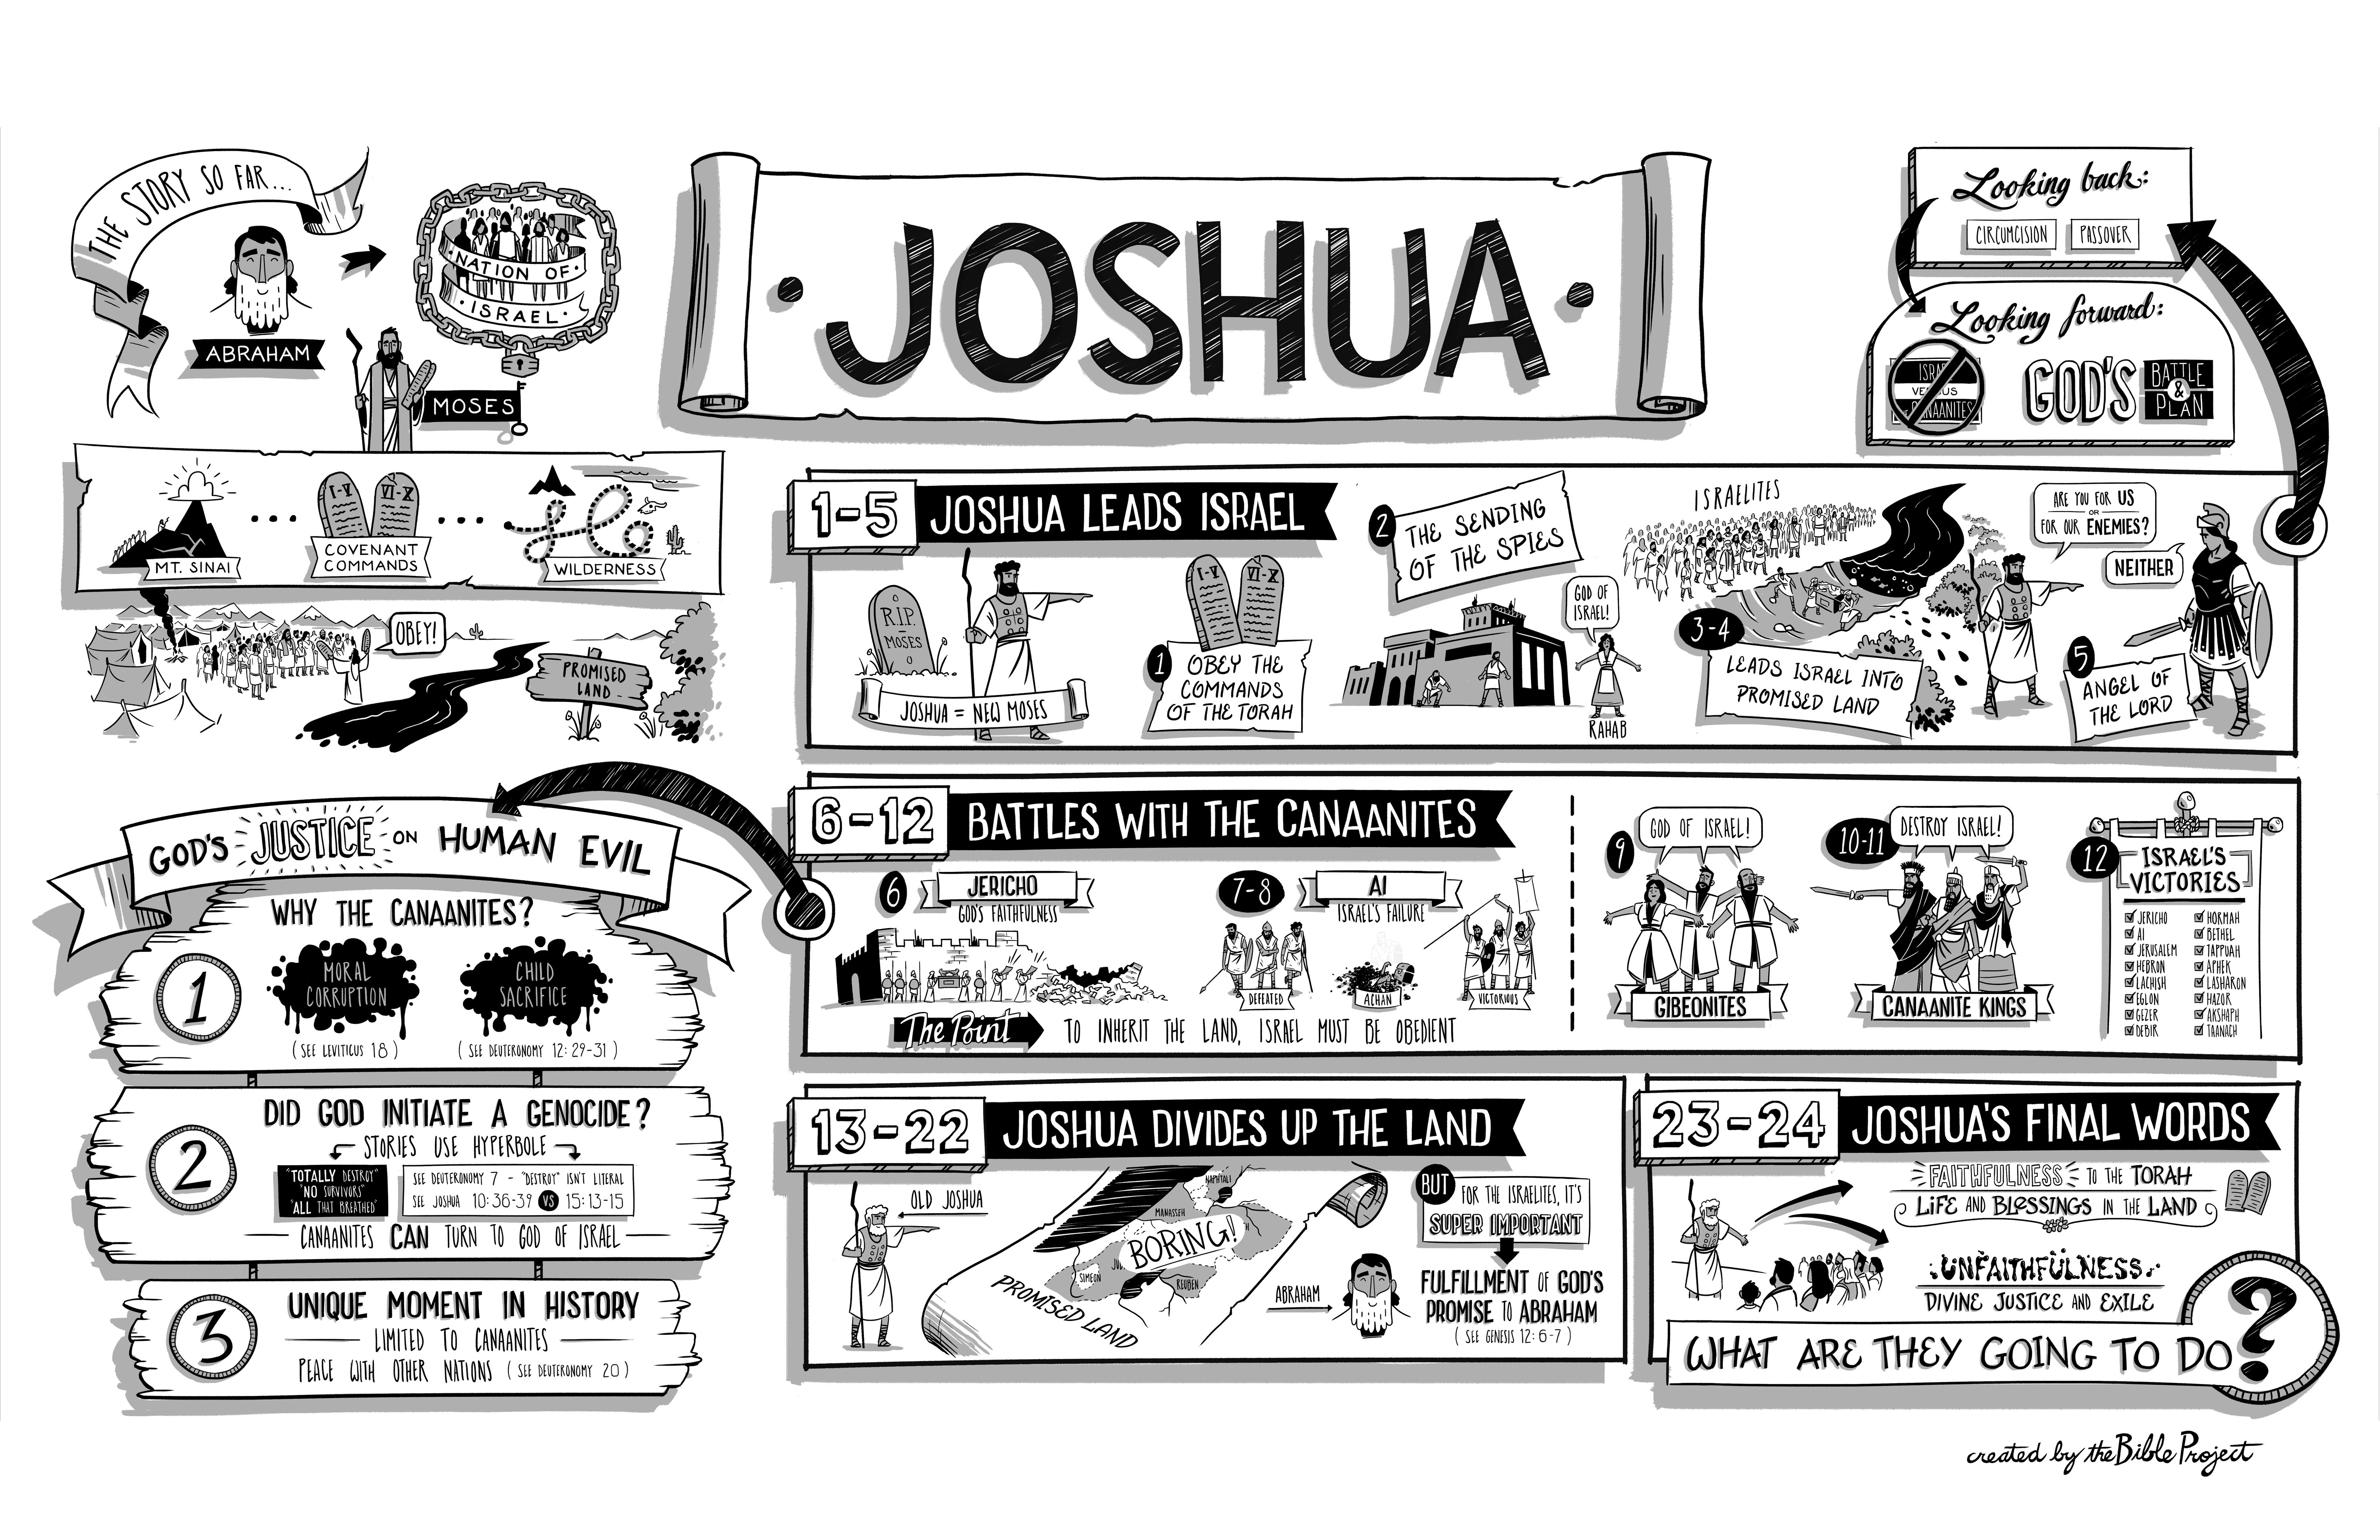
\includegraphics[scale=0.5, angle=90]{06OT-Joshua/References/1.BibleProject-Joshua.jpg}
\caption[Joshua from the Bible Project]{Joshua from the Bible Project}
\label{fig:Joshua from the Bible Project}
\end{center}
\end{figure}

\newpage
\begin{figure}
\begin{center}
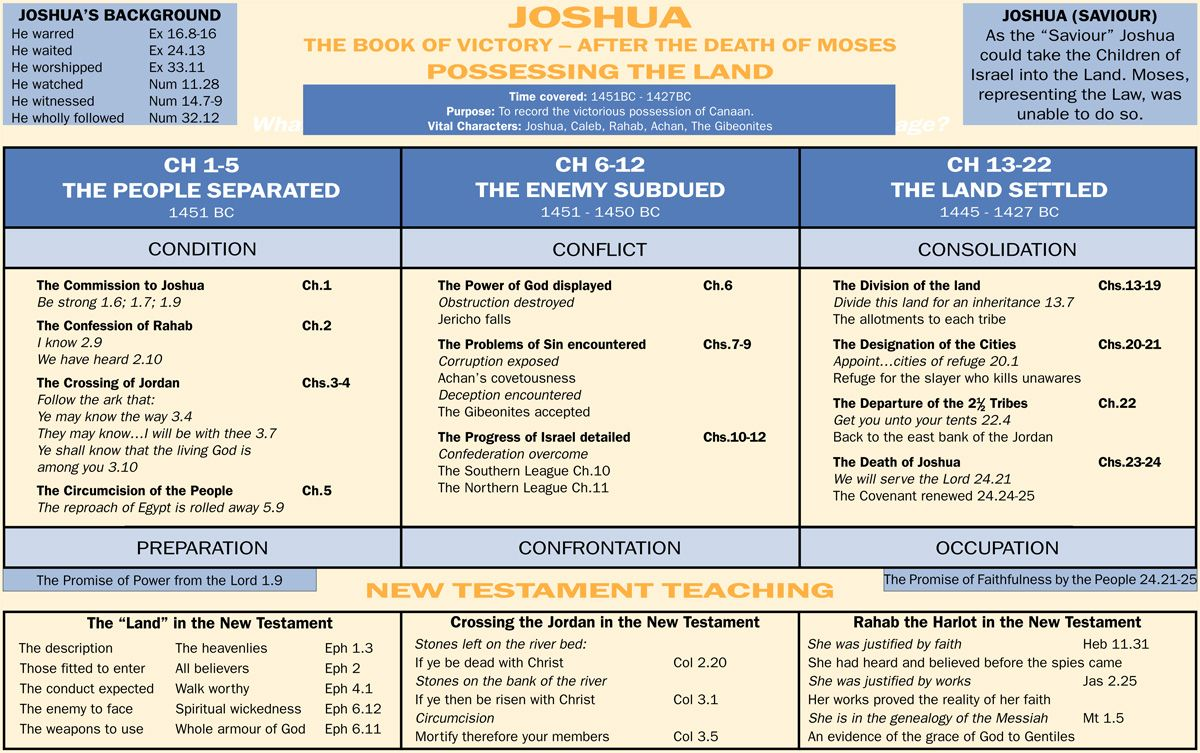
\includegraphics[scale=0.5, angle=90]{06OT-Joshua/References/2.JohnGrant-Joshua.jpg}
\caption[Joshua from John Grant]{Joshua from John Grant}
\label{fig:Joshua from John Grant}
\end{center}
\end{figure}

\newpage
\begin{figure}
\begin{center}
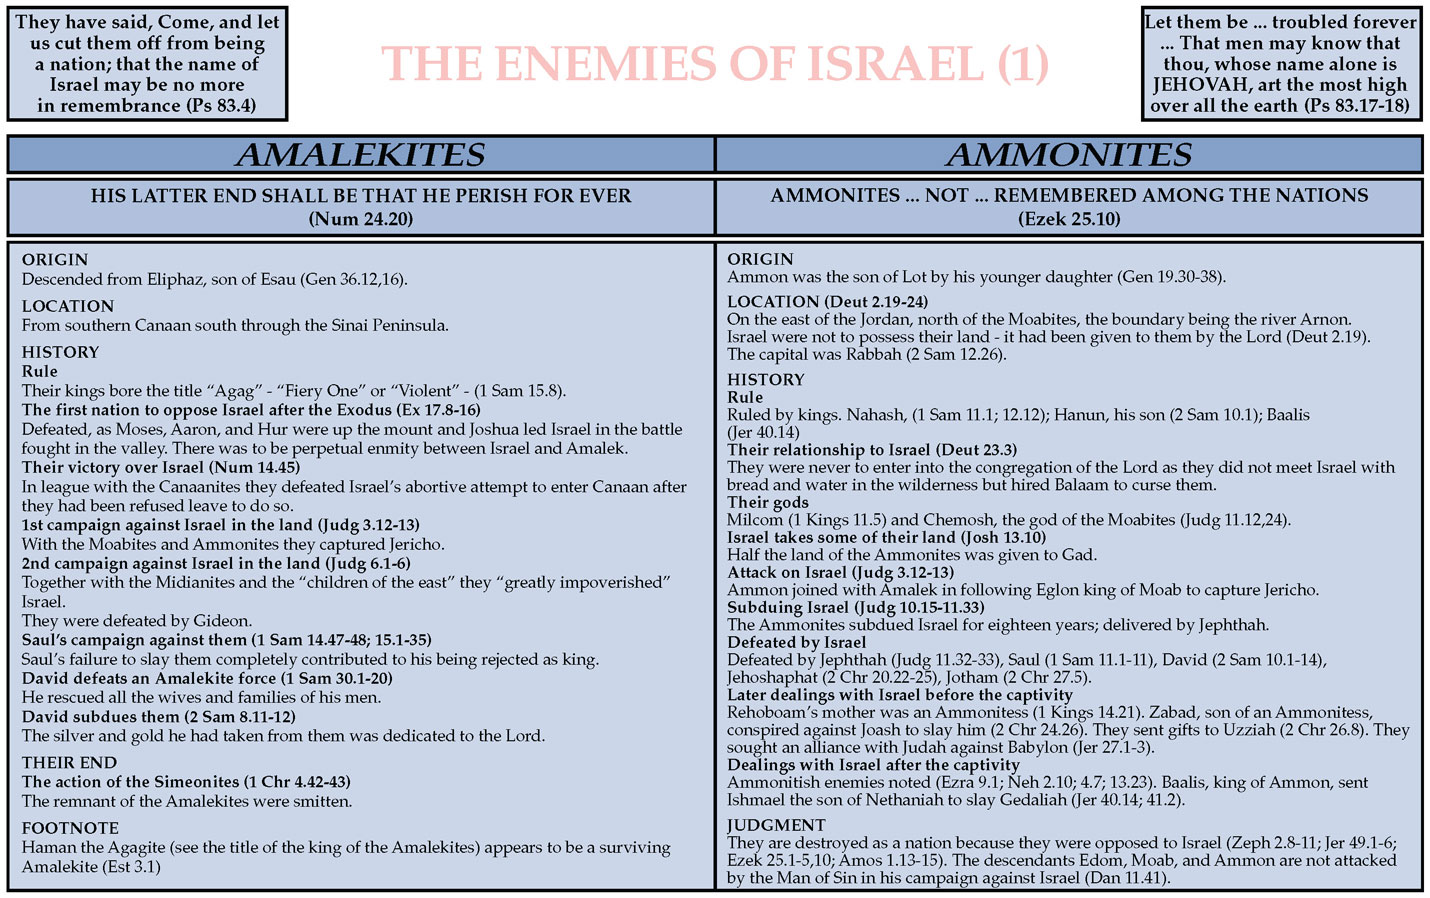
\includegraphics[scale=0.4, angle=90]{06OT-Joshua/References/3.EnemiesOfIsrael1.jpg}
\caption[Enemies of Israel 1]{Enemies of Israel 1}
\label{fig:Enemies of Israel 1}
\end{center}
\end{figure}

\newpage
\begin{figure}
\begin{center}
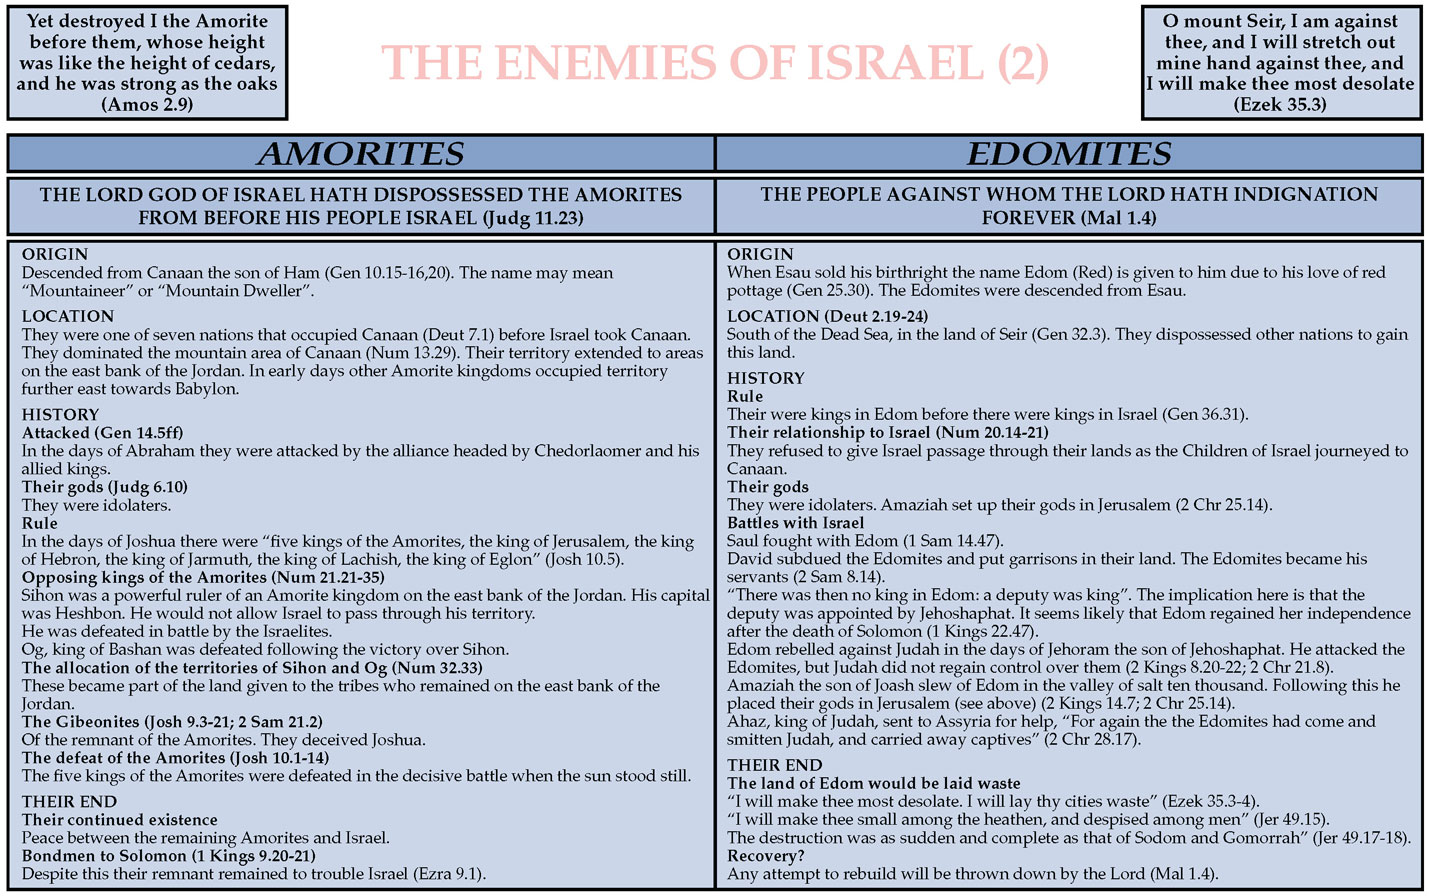
\includegraphics[scale=0.4, angle=90]{06OT-Joshua/References/4.EnemiesOfIsrael2.jpg}
\caption[Enemies of Israel 2]{Enemies of Israel 2}
\label{fig:Enemies of Israel 2}
\end{center}
\end{figure}

\newpage
\begin{figure}
\begin{center}
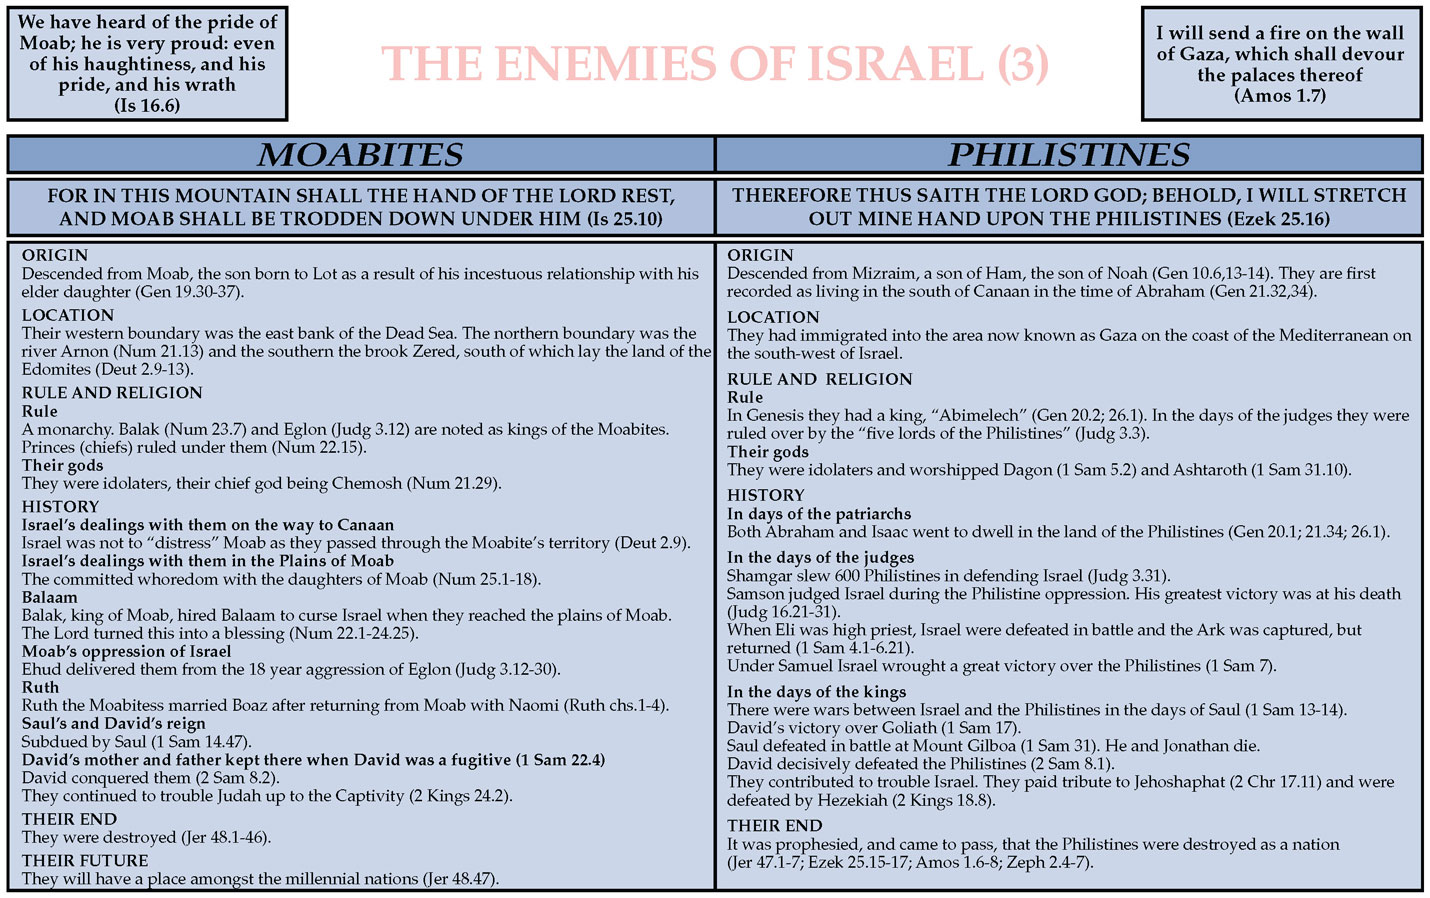
\includegraphics[scale=0.4, angle=90]{06OT-Joshua/References/5.EnemiesOfIsrael3.jpg}
\caption[Enemies of Israel 3]{Enemies of Israel 3}
\label{fig:Enemies of Israel 3}
\end{center}
\end{figure}

\newpage
\begin{figure}
\begin{center}
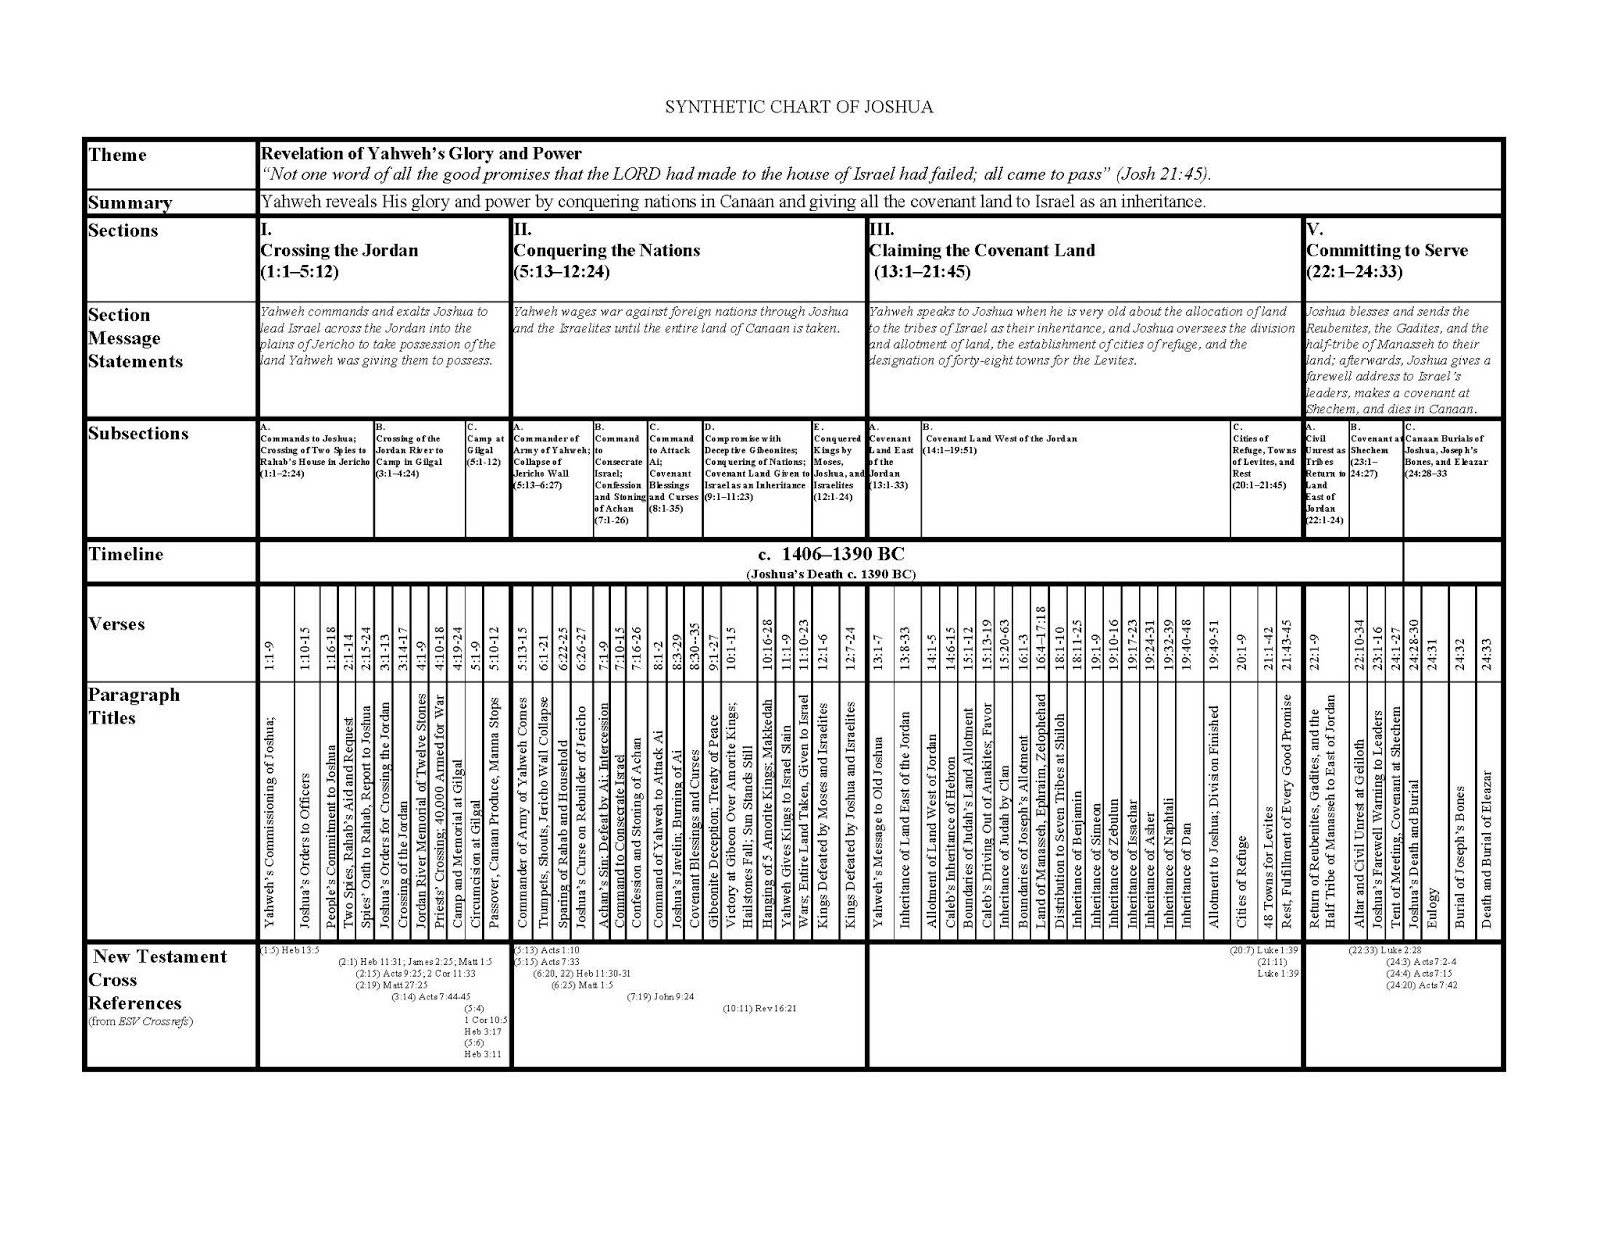
\includegraphics[scale=.4, angle=90]{06OT-Joshua/References/6.SyntheticChartofJoshua.jpg}
\caption[Synthetic Chart of Joshua]{Synthetic Chart of Joshua}
\label{fig:Synthetic Chart of Joshua}
\end{center}
\end{figure}


\newpage
\begin{figure}
\begin{center}
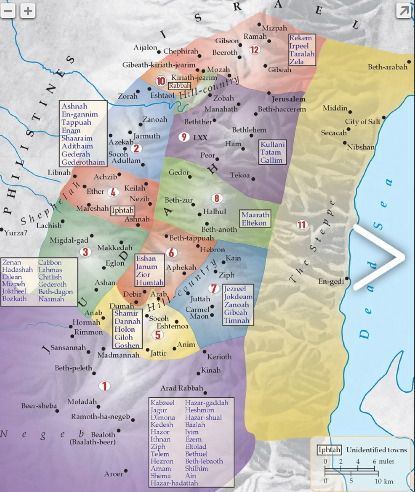
\includegraphics[scale=1, angle=0]{06OT-Joshua/References/7.WestSideOfDeadSea.jpg}
\caption[The West Side of the Dead Sea]{The West Side of the Dead Sea}
\label{fig:The West Side of the Dead Sea}
\end{center}
\end{figure}


\newpage
\begin{figure}
\begin{center}
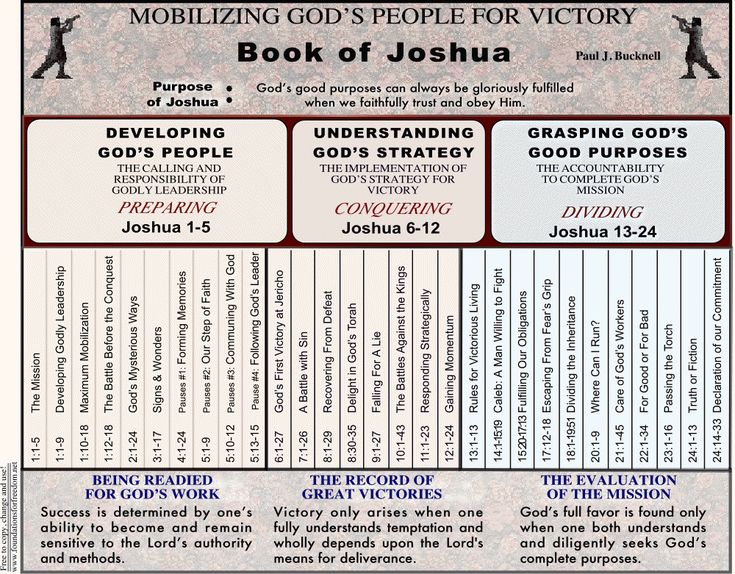
\includegraphics[scale=0.75, angle=90]{06OT-Joshua/References/8.Bucknell-Joshua.jpg}
\caption[Joshua from Bucknell]{Joshua from Bucknell}
\label{fig:Joshua from Bucknell}
\end{center}
\end{figure}


%\newpage
%\begin{figure}
%\begin{center}
%\includegraphics[scale=2, angle=90]{06OT-Joshua/References/9.Jensen-Joshua.png}
%\caption[Joshua from Jensen]{Joshua from Jensen}
%\label{fig:Joshua from Jensen}
%\end{center}
%\end{figure}


\newpage
\begin{figure}
\begin{center}
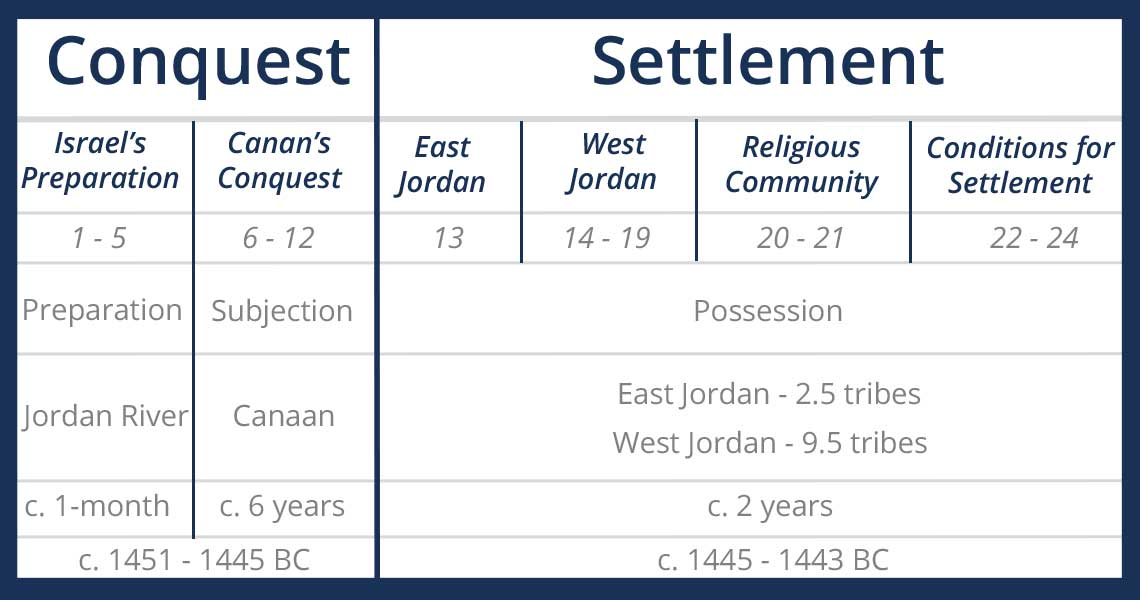
\includegraphics[scale=.5, angle=90]{06OT-Joshua/References/10.Bible-Brief-Joshua.jpg}
\caption[Bible Brief for Joshua]{Bible Brief for Joshua}
\label{fig:Bible Brief for Joshua}
\end{center}
\end{figure}

\newpage
\begin{figure}
\begin{center}
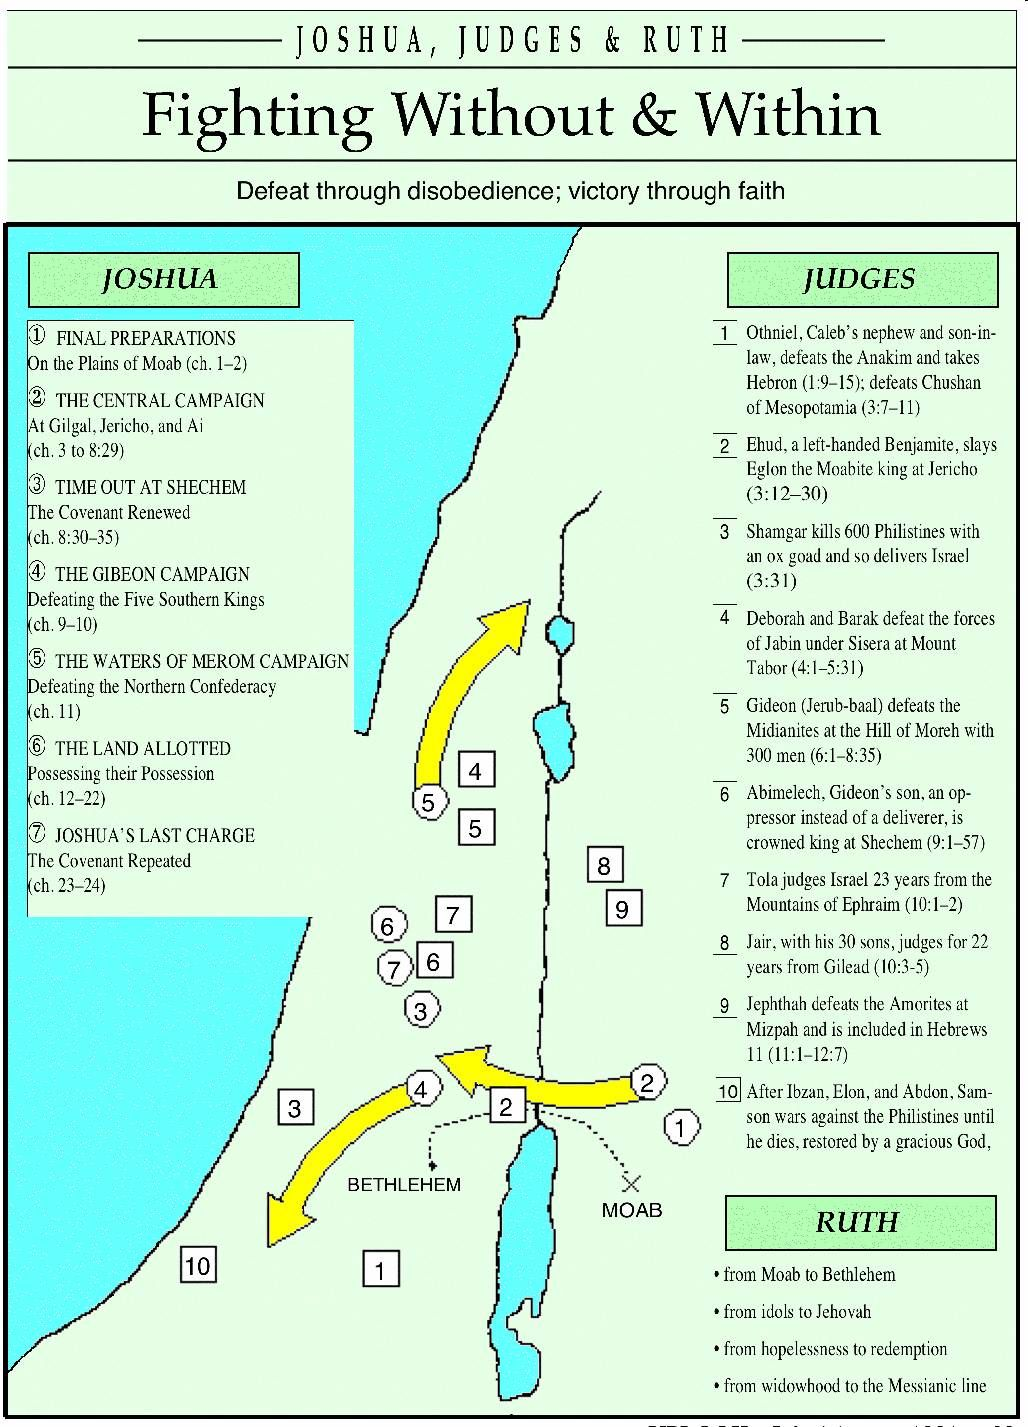
\includegraphics[scale=.5, angle=0]{06OT-Joshua/References/11.FightingInJoshuaAndJudges.jpg}
\caption[The Fighting in Joshua and Judges]{The Fighting in Joshua and Judges}
\label{fig:The Fighting in Joshua and Judges}
\end{center}
\end{figure}

\newpage
\begin{figure}
\begin{center}
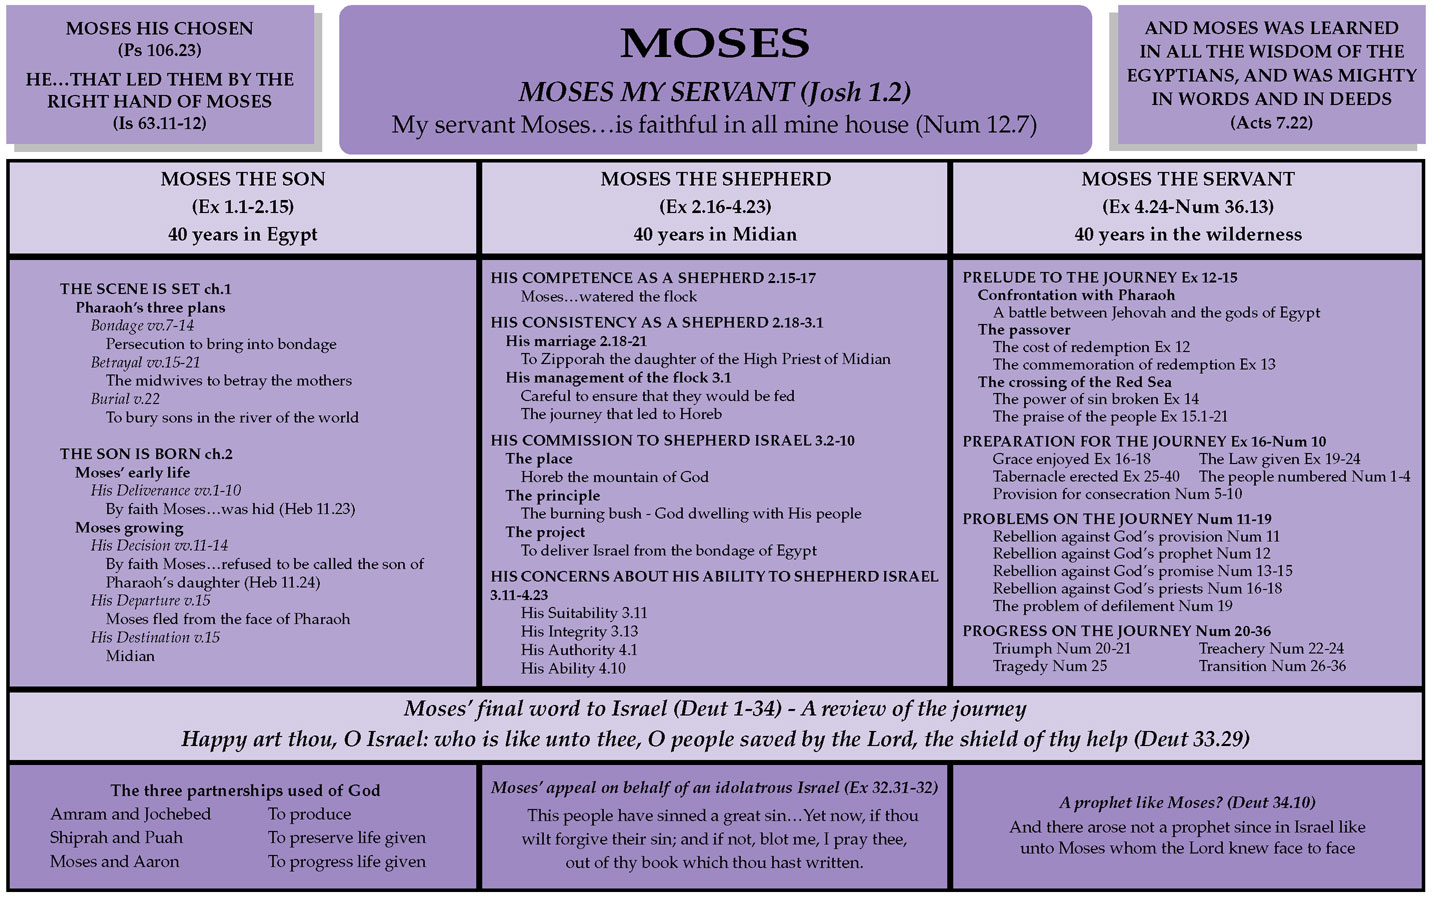
\includegraphics[scale=.4, angle=90]{06OT-Joshua/References/12.JohnGrantMoses.jpg}
\caption[Moses from John Grant]{Moses from John Grant}
\label{fig:Moses from John Grant}
\end{center}
\end{figure}







\chapter{Psalm 76}

\begin{figure}
  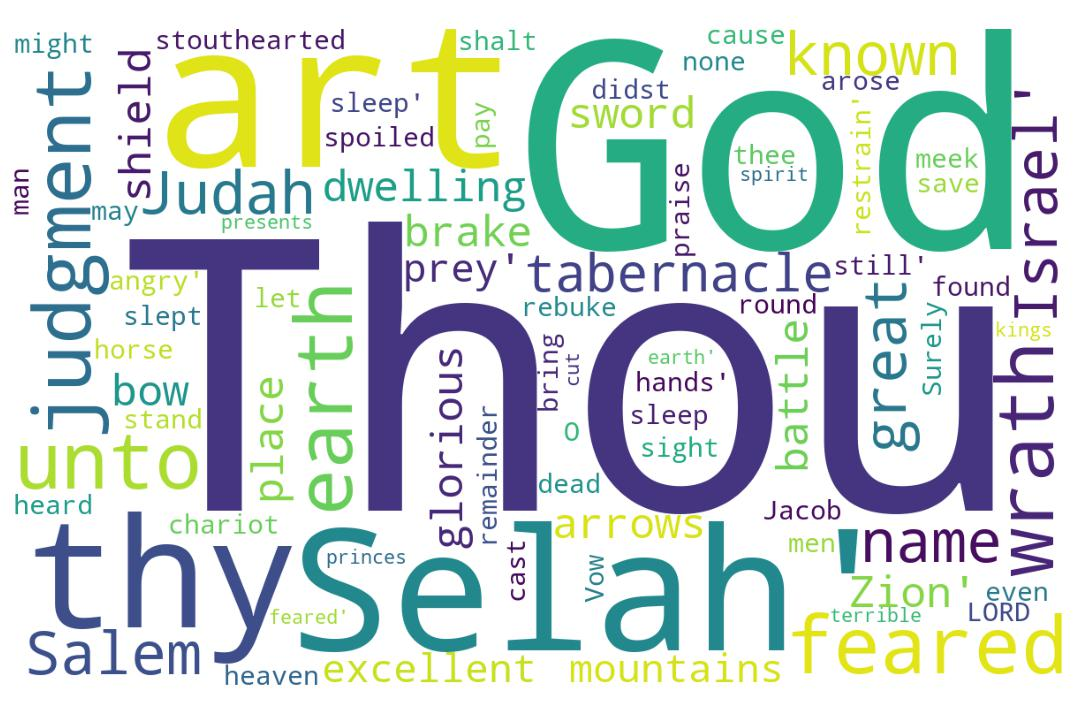
\includegraphics[width=\linewidth]{19OT-Psalms/Psalm76-WordCloud.jpg}
  \caption{Psalm 76 Word Cloud}
  \label{fig:Psalm 76 word Cloud}
\end{figure}

\marginpar{\scriptsize \centering \fcolorbox{bone}{lime}{\textbf{TWO KINDS OF PEOPLE}}\\ (Psalm 76:1-12) \begin{compactenum}[I.][8]
     \item Those \textbf{Shielded} \index[scripture]{Psalms!Psa 076:03}(Psa 76:3)
    \item Those \textbf{Spoiled} \index[scripture]{Psalms!Psa 076:05}(Psa 76:5)
    \item Those \textbf{Put to Sleep} \index[scripture]{Psalms!Psa 076:06}(Psa 76:6)
    \item Those \textbf{Seen} \index[scripture]{Psalms!Psa 076:07}(Psa 76:7)
    \item Those \textbf{Stilled} \index[scripture]{Psalms!Psa 076:08}(Psa 76:8)
    \item Those \textbf{Subdued} \index[scripture]{Psalms!Psa 076:08}(Psa 76:8)
    \item Those \textbf{Saved} \index[scripture]{Psalms!Psa 076:09}(Psa 76:9)
\end{compactenum}}
    




% \textcolor[cmyk]{0.99998,1,0,0}{
\footnote{\textcolor[rgb]{0.00,0.25,0.00}{\hyperlink{TOC}{Return to end of Table of Contents.}}}\footnote{\href{https://audiobible.com/bible/psalms_76.html}{\textcolor[cmyk]{0.99998,1,0,0}{Psalm 76 Audio}}}\textcolor[cmyk]{0.99998,1,0,0}{To the chief Musician on Neginoth, A Psalm \emph{or} Song of Asaph.}\\
\\
\textcolor[cmyk]{0.99998,1,0,0}{In Judah \emph{is} God known: his name \emph{is} great in Israel.} %\footnote{[RUCKMAN] The Psalm is on the Second Advent. God is not known in Judah now, nor has His ``name'' been ``great in Israel'' for 1,950 years. The name “Jehovah” may be great in Israel now, but if we are to believe Deuteronomy 32:15--22; Mark 7:3--13; and Romans 10:1--3, the name is only lip service. God is NOT known, and will not be “known in Judah and Israel” until Hebrews 8:8--12. In this age, God is known, and His “name is great,” among the Gentiles (Acts 28:28), but only because of the Jew (“Judah”). The term “Jew” was given to Judean Jews in Jerusalem (John 5:16, 18), and inspite of tons of anti-Semitic hogwash about “Khazars,” “Edomite usurpers,” and the “ten lost tribes,” salvation is still of the “Jews,” and I don’t mean “Israel” or “the Israel of God” or the “house of Israel.” I mean “Jews,” as in Judean Jews from Judah (vs. 1).\cite{Ruckman1992Psalms}}
[2] \textcolor[cmyk]{0.99998,1,0,0}{In Salem also is his tabernacle, and his dwelling place in Zion.} %\footnote{[RUCKMAN] ``In Salem.” The word is kin to “Shalom” and “Shiloh,” meaning “peace.” God’s dwelling place in this age is NOT in Zion, and He has no tabernacle there; Asaph is prophesying (see the introductory notes). Those who tried to historicize verse 2, and lay it on David or Solomon, have two problems. In the first place, wars do NOT stop in David’s time, nor do they stop in Solomon’s time. The breaking up of weapons in verse 3 is punctuated by our good, old friend “Selah,” showing anyone but a Bible-correcting Hebrew scholar that we are to look at Haggai 2:9 and Zechariah 14 for the meaning of the verse. The word Jerusalem means “city of peace,” so:\cite{Ruckman1992Psalms}
%\begin{compactenum}
%\item It is captured by the Jews in Judges 1:8, but they have to fight against it again to retake it in 2 Samuel 5:6–10. 
%\item Shishak attacks it in 2 Chronicles 12:9.
%\item Jehoash goes after it in 2 Kings 14:13, Rezin in 2 Kings 16:5, and Sennacherib in Isaiah 36 and 37.
%\end{compactenum} 
%Nebuchadnezzar goes up to it three times; Ptolemy Soter attacks it in 320 B.C., Antiochus defiles it in 203 B.C., Scopus attacks it in 199 B.C., and Antiochus hits it again in 168 B.C., and then again “for good measure” in 162 B.C. “City of Peace.” Fantastic, isn’t it? Imagine the commentators thinking that God stopped all the wars with the destruction of David’s foes or Solomon’s or even Hezekiah’s foes (Sennacherib)! Kroll is as tongue tied when he stares at the passage as a calf looking at a “new gate.” He doesn’t know what on earth to do with it. Hyracannus attacks Jerusalem in 65 B.C. Pompey follows suit in 63 B. C. Herod does a bang up job in 39 B.C., and then Titus finishes it off in A.D. 70. But the best is yet to come. Chosroes the Persian attacks it in A.D. 559 after the Romans did it in A.D. 135. Then Afdal takes it in A.D. 1098, after Omar destroyed it in A.D. 637. Then the Crusaders take it (A.D. 1099) only to lose it to Saladin (A.D. 1187). Never fear. Allenby “liberated” it in A.D. 1917, and then the Arabs took over fighting against it with Lebanese, Egyptians, the PLO, the Pope, and the American news media to help them out.\cite{Ruckman1992Psalms}}
[3] \textcolor[cmyk]{0.99998,1,0,0}{There brake he the arrows of the bow, the \fcolorbox{bone}{lime}{shield}, and the sword, and the battle. Selah.}
[4] \textcolor[cmyk]{0.99998,1,0,0}{Thou \emph{art} more glorious \emph{and} excellent than the mountains of prey.} %\footnote{[RUCKMAN] The “thou” is Mt. Zion (see Ps. 68:15 and comments). Two thoughts are present. Mountains which have wild animals on them who take “prey” (Song of Sol. 4:8), are not to be compared with a mountain like Mt. Zion, which not only had the temple on the place where God ordained sacrifices to be made, but also was the location of the Ark of the Covenant which held the Book (Deut. 31:26). The “oracle” of God (1 Kings 6:5) was located on Mt. Zion. The second thought is that the earthly powers represented by mountains (see Rev. 17, for example, and Jeremiah 51:25) are no equal for the “mountain of the Lord” (see Isa. 2:2). He is “king of the mountain,” and His “mountain” will tower above McKinley, Blanc, Whitney, Ararat, Everest, etc., for its prototype (see Heb. 12:22) is already a good bit higher than the entire Milky Way.\cite{Ruckman1992Psalms}}
[5] \textcolor[cmyk]{0.99998,1,0,0}{The stouthearted are \fcolorbox{bone}{lime}{spoiled}, they have slept their sleep: and none of the men of might have found their hands.} %\footnote{[RUCKMAN] Literally, in the sense of Saul (1 Sam. 26:12), who is a type of the Antichrist; doctrinally, in the sense of being dead (see Isa. 26:14; Dan. 12:2). Several things happen at Armageddon that the prophetic expositors never picked up. One of them is that the Antichrist’s troops will kill each other (Judg. 7:22), their flesh will rot on their faces (Zech. 14:12), and their horses will go blind and rabid in the midst of the attack (Zech. 12:4). These are the UN troops (Rev. 19:19) who hope to overthrow the rider on the “white horse” (Rev. 19:10-–14). Observe the advanced revelation found in the AV text which all of the commentators (naturally) missed. When Kroll sees that the “chariot” goes into a dead sleep, as well as the “horses” he mumbles, “the cavalries of the oppressors were stopped.” (Yeah, sonny, they sure were.) The New Idiotic Version (NIV) can’t handle it, so they say that “they lie still.” The Living Baboon says “fell.” The RSV, NRSV, NNRSV (and NNNRSV) take the word “chariot” clean out of the text so they don’t have to deal with the problem: “Both rider and horse lay stunned.” Typical. Absolutely typical of the brand of scholarship you would get at Bob Jones or Liberty University. \cite{Ruckman1992Psalms}}
[6] \textcolor[cmyk]{0.99998,1,0,0}{At thy rebuke, O God of Jacob, both the chariot and horse are cast into a \fcolorbox{bone}{lime}{dead sleep}.} %\footnote{[RUCKMAN] But after 1910, the “chariot” could go to “sleep.” What auto mechanic doesn’t know that? As a matter of fact, the motor can even “die,” and what driver didn’t know that? If it is “awake” but not moving, it is “idling,” and who didn’t know that but the commentators who couldn’t imagine chariots going to sleep? They went to sleep on the Russian front (1942--1944) because the tank fluids froze, or the rats shortcircuited the controls by chewing through the insulation. In my generation (1921--1949), we called automobiles by a peculiar name; we called them “chariots.” A chariot can “malfunction.”\cite{Ruckman1992Psalms}}
[7] \textcolor[cmyk]{0.99998,1,0,0}{Thou, \emph{even} thou, \emph{art} to be feared: and who may stand \fcolorbox{bone}{lime}{in thy sight} when once thou art angry?}
[8] \textcolor[cmyk]{0.99998,1,0,0}{Thou didst cause judgment to be heard from heaven; the earth feared, and was \fcolorbox{bone}{lime}{still}.}
[9] \textcolor[cmyk]{0.99998,1,0,0}{When God arose to judgment, to \fcolorbox{bone}{lime}{save} all the meek of the earth. \fcolorbox{bone}{red}{\textcolor{white}{Selah}}.} %\footnote{[RUCKMAN] All is clear. God “arises” in verse 9 (see Ps. 3:7, 7:6, and 9:19), and not one time is this a reference to God helping anyone out between 500 B. C. and A.D. 2002. “Selah” comes to our aid again to give us the key for judging the critics of the Book. It is a “handy reference” to use in throwing out 80 percent of the rubbish on the Psalms published by Zondervan, Baker, Eerdmans, and Bob Jones University Press. Verse 11 is the exact match for the comments under Psalm 68:29--32, which see. The “vow” of verse 11 is the exact millennial match to Psalm 65:1 and Psalm 50:14, which see. Verse 12 is Armageddon fulfilled, as in Psalm 2:2, 89:27, and Isaiah 24:21. This is a literal destruction at the Advent. In verse 8, we learn that the earth has more sense than most of its inhabitants. The judgment is “heard from heaven,” literally, in Hebrews 12:25; Haggai 2:6; and Psalm 50:3--5 (which see). All of the commentators miss all the references. (This is just as natural for them as breathing.) Note “the meek” of the Sermon on the Mount (Matt. 5:5), showing up in verse 9. \cite{Ruckman1992Psalms}}
[10] \textcolor[cmyk]{0.99998,1,0,0}{Surely the wrath of man shall praise thee: the remainder of wrath shalt thou restrain.} %\footnote{[RUCKMAN ]The destructive critics of the AV come apart at verse 10, which stands in the AV as clear as crystal. The idea is that man’s hatred against God and God’s people will be turned backwards, so that instead of destroying God’s people or stopping God’s hand, God “banks it off the siderail”—He winds up getting glory from it (see Exod. 14:4; Rom. 11:30–34; and Exod. 9:16, 18:11). “The remainder” is a reference to any wrath that does not produce praise for God or glory to Him. Cases are too numerous to mention, the main ones being men killing each other over religious and political issues to the tune of 80,000,000 casualties since A.D. 70. Individual murders (five a day in Detroit, one a day in Las Vegas, two a day in Miami, and ten a day in Washington, D.C.) do not praise God, but murderers are restrained so that total mayhem and murder don’t break out internationally with five hundred killed daily in Memphis, Atlanta, London, Paris, New York, Rome, Madrid, Tokyo, Bombay, Athens, Oslo, Seattle, and Oklahoma City. What wrath does not praise God is held in check so it doesn’t annihilate mankind altogether. Today the Arabs are restrained by “the restrainer” (2 Thess. 2:6–7); otherwise, they would have pushed Israel off into the Mediterranean more than sixty years ago. Kroll (LU) can’t handle it. His peers (Falwell and company) printed a NKJV that reads “you shall gird yourself.” But having made this change, in line with most “highly qualified, recognized Hebrew scholarship” available--used in the RSV, NRSV, and NIV-- they are powerless to interpret the mess they produced, so they leave it there like a rotten egg and print the AV text in the commentary, and then refuse to comment on it! Liberty University inherited its corruption from Edward Wetenhall, the Lord Bishop of Corke and Rosse (1661), Cornelius Buges (1614), and Maurer. These gentlemen tell us that “the Hebrew says....” (Oh, don’t you know. Don’t you just know “the Hebrew says.” I know what “the Hebrew says.” It says whatever the Cult wants you to think it should say. You don’t fool me, kiddies. I used to bartend and lifeguard for a living. You don’t fool me. I’ve shot craps in the alley, played poker “below decks,” got drunk in the French Quarter, and played “cops and teen agers” at all hours of the night. Don’t kid me. I know what the “Hebrew” better say, even if it doesn’t say it.) “Probably it is meant that God girds himself with the praise to which the last of the enemy even to its last remnant is constrained to minister, both in the case of reprobates and....” Yep; that is exactly what it didn’t say, and that is exactly what it didn’t mean. “This, in the Hebrew, is expressed in one word...which imports the begirding or binding of it on every side, that it shall by no means break out, but shall be kept in, as a dog on a chain....” Oh, I got it! He is “held in restraint”! He is a “restrainer”; a leash. Oh yeah, I got “the Hebrew” now! It didn’t mean “gird” at all. It meant “the remainder of wrath shalt thou restrain.” (That’s what I thought you said.) The Living Bible says the “remainder” is an “ornament,” and the Nitty Ickey Version (NIV) says that some “survivors” of God’s wrath are restrained. In the Asinine Standard Vision (ASV), God girds Himself with wrath that came from men instead of Himself. Ditto the Rotten Stupid Version (RSV). Stupidity is infectious. It is passed reverently from one generation of “godly” men to another, so that “historic positions” can overthrow the truth of God in each generation. \cite{Ruckman1992Psalms} }
[11] \textcolor[cmyk]{0.99998,1,0,0}{Vow, and pay unto the LORD your God: let all that be round about him bring presents unto him that ought to be feared.} %\footnote{[RUCKMAN] The ``earth feared'' because the Lord is the One ``that ought to be feared'' (vs. 11). This is for a number of reasons:\cite{Ruckman1992Psalms}
%\begin{compactenum}
%\item He will break all your weapons of war in pieces no matter how “advanced” they are.
%\item He can cast you into a deep sleep (Acts 12:6; Matt. 25:5) when you need to be awake.
%\item He will cut off world rulers, in terror, even if they are ``kings'' and ``princes.''
%\item He can cast you out of His sight and destroy both body and soul in Hell (Matt. 10:28).
%\end{compactenum}}
[12] \textcolor[cmyk]{0.99998,1,0,0}{He shall cut off the spirit of princes: \emph{he} \emph{is} terrible to the kings of the earth.}
\section{Psalm 76 Comments}




%\index[NWIV]{11!Psalms!Psa 76:1}\index[AWIP]{In!Psalms!Psa 76:1}\index[AWIP]{Judah!Psalms!Psa 76:1}\index[AWIP]{\emph{is}!Psalms!Psa 76:1}\index[AWIP]{\emph{is}!Psalms!Psa 76:1 (2)}\index[AWIP]{God!Psalms!Psa 76:1}\index[AWIP]{known!Psalms!Psa 76:1}\index[AWIP]{his!Psalms!Psa 76:1}\index[AWIP]{name!Psalms!Psa 76:1}\index[AWIP]{great!Psalms!Psa 76:1}\index[AWIP]{in!Psalms!Psa 76:1}\index[AWIP]{Israel!Psalms!Psa 76:1}\index[AWIP]{\emph{is}!Psalms!Psa 76:1}\index[AWIP]{\emph{is}!Psalms!Psa 76:1 (2)}

\index[NWIV]{12!Psalms!Psa 76:2}\index[AWIP]{In!Psalms!Psa 76:2}\index[AWIP]{Salem!Psalms!Psa 76:2}\index[AWIP]{also!Psalms!Psa 76:2}\index[AWIP]{is!Psalms!Psa 76:2}\index[AWIP]{his!Psalms!Psa 76:2}\index[AWIP]{his!Psalms!Psa 76:2 (2)}\index[AWIP]{tabernacle!Psalms!Psa 76:2}\index[AWIP]{and!Psalms!Psa 76:2}\index[AWIP]{dwelling!Psalms!Psa 76:2}\index[AWIP]{place!Psalms!Psa 76:2}\index[AWIP]{in!Psalms!Psa 76:2}\index[AWIP]{Zion!Psalms!Psa 76:2}

\index[NWIV]{17!Psalms!Psa 76:3}\index[AWIP]{There!Psalms!Psa 76:3}\index[AWIP]{brake!Psalms!Psa 76:3}\index[AWIP]{he!Psalms!Psa 76:3}\index[AWIP]{the!Psalms!Psa 76:3}\index[AWIP]{the!Psalms!Psa 76:3 (2)}\index[AWIP]{the!Psalms!Psa 76:3 (3)}\index[AWIP]{the!Psalms!Psa 76:3 (4)}\index[AWIP]{the!Psalms!Psa 76:3 (5)}\index[AWIP]{arrows!Psalms!Psa 76:3}\index[AWIP]{of!Psalms!Psa 76:3}\index[AWIP]{bow!Psalms!Psa 76:3}\index[AWIP]{shield!Psalms!Psa 76:3}\index[AWIP]{and!Psalms!Psa 76:3}\index[AWIP]{and!Psalms!Psa 76:3 (2)}\index[AWIP]{sword!Psalms!Psa 76:3}\index[AWIP]{battle!Psalms!Psa 76:3}\index[AWIP]{Selah!Psalms!Psa 76:3}

\index[NWIV]{11!Psalms!Psa 76:4}\index[AWIP]{Thou!Psalms!Psa 76:4}\index[AWIP]{\emph{art}!Psalms!Psa 76:4}\index[AWIP]{more!Psalms!Psa 76:4}\index[AWIP]{glorious!Psalms!Psa 76:4}\index[AWIP]{\emph{and}!Psalms!Psa 76:4}\index[AWIP]{excellent!Psalms!Psa 76:4}\index[AWIP]{than!Psalms!Psa 76:4}\index[AWIP]{the!Psalms!Psa 76:4}\index[AWIP]{mountains!Psalms!Psa 76:4}\index[AWIP]{of!Psalms!Psa 76:4}\index[AWIP]{prey!Psalms!Psa 76:4}\index[AWIP]{\emph{art}!Psalms!Psa 76:4}\index[AWIP]{\emph{and}!Psalms!Psa 76:4}

\index[NWIV]{20!Psalms!Psa 76:5}\index[AWIP]{The!Psalms!Psa 76:5}\index[AWIP]{stouthearted!Psalms!Psa 76:5}\index[AWIP]{are!Psalms!Psa 76:5}\index[AWIP]{spoiled!Psalms!Psa 76:5}\index[AWIP]{they!Psalms!Psa 76:5}\index[AWIP]{have!Psalms!Psa 76:5}\index[AWIP]{have!Psalms!Psa 76:5 (2)}\index[AWIP]{slept!Psalms!Psa 76:5}\index[AWIP]{their!Psalms!Psa 76:5}\index[AWIP]{their!Psalms!Psa 76:5 (2)}\index[AWIP]{sleep!Psalms!Psa 76:5}\index[AWIP]{and!Psalms!Psa 76:5}\index[AWIP]{none!Psalms!Psa 76:5}\index[AWIP]{of!Psalms!Psa 76:5}\index[AWIP]{of!Psalms!Psa 76:5 (2)}\index[AWIP]{the!Psalms!Psa 76:5}\index[AWIP]{men!Psalms!Psa 76:5}\index[AWIP]{might!Psalms!Psa 76:5}\index[AWIP]{found!Psalms!Psa 76:5}\index[AWIP]{hands!Psalms!Psa 76:5}

\index[NWIV]{18!Psalms!Psa 76:6}\index[AWIP]{At!Psalms!Psa 76:6}\index[AWIP]{thy!Psalms!Psa 76:6}\index[AWIP]{rebuke!Psalms!Psa 76:6}\index[AWIP]{O!Psalms!Psa 76:6}\index[AWIP]{God!Psalms!Psa 76:6}\index[AWIP]{of!Psalms!Psa 76:6}\index[AWIP]{Jacob!Psalms!Psa 76:6}\index[AWIP]{both!Psalms!Psa 76:6}\index[AWIP]{the!Psalms!Psa 76:6}\index[AWIP]{chariot!Psalms!Psa 76:6}\index[AWIP]{and!Psalms!Psa 76:6}\index[AWIP]{horse!Psalms!Psa 76:6}\index[AWIP]{are!Psalms!Psa 76:6}\index[AWIP]{cast!Psalms!Psa 76:6}\index[AWIP]{into!Psalms!Psa 76:6}\index[AWIP]{a!Psalms!Psa 76:6}\index[AWIP]{dead!Psalms!Psa 76:6}\index[AWIP]{sleep!Psalms!Psa 76:6}

\index[NWIV]{19!Psalms!Psa 76:7}\index[AWIP]{Thou!Psalms!Psa 76:7}\index[AWIP]{\emph{even}!Psalms!Psa 76:7}\index[AWIP]{thou!Psalms!Psa 76:7}\index[AWIP]{thou!Psalms!Psa 76:7 (2)}\index[AWIP]{\emph{art}!Psalms!Psa 76:7}\index[AWIP]{to!Psalms!Psa 76:7}\index[AWIP]{be!Psalms!Psa 76:7}\index[AWIP]{feared!Psalms!Psa 76:7}\index[AWIP]{and!Psalms!Psa 76:7}\index[AWIP]{who!Psalms!Psa 76:7}\index[AWIP]{may!Psalms!Psa 76:7}\index[AWIP]{stand!Psalms!Psa 76:7}\index[AWIP]{in!Psalms!Psa 76:7}\index[AWIP]{thy!Psalms!Psa 76:7}\index[AWIP]{sight!Psalms!Psa 76:7}\index[AWIP]{when!Psalms!Psa 76:7}\index[AWIP]{once!Psalms!Psa 76:7}\index[AWIP]{art!Psalms!Psa 76:7}\index[AWIP]{angry?!Psalms!Psa 76:7}\index[AWIP]{\emph{even}!Psalms!Psa 76:7}\index[AWIP]{\emph{art}!Psalms!Psa 76:7}

\index[NWIV]{15!Psalms!Psa 76:8}\index[AWIP]{Thou!Psalms!Psa 76:8}\index[AWIP]{didst!Psalms!Psa 76:8}\index[AWIP]{cause!Psalms!Psa 76:8}\index[AWIP]{judgment!Psalms!Psa 76:8}\index[AWIP]{to!Psalms!Psa 76:8}\index[AWIP]{be!Psalms!Psa 76:8}\index[AWIP]{heard!Psalms!Psa 76:8}\index[AWIP]{from!Psalms!Psa 76:8}\index[AWIP]{heaven!Psalms!Psa 76:8}\index[AWIP]{the!Psalms!Psa 76:8}\index[AWIP]{earth!Psalms!Psa 76:8}\index[AWIP]{feared!Psalms!Psa 76:8}\index[AWIP]{and!Psalms!Psa 76:8}\index[AWIP]{was!Psalms!Psa 76:8}\index[AWIP]{still!Psalms!Psa 76:8}

\index[NWIV]{14!Psalms!Psa 76:9}\index[AWIP]{When!Psalms!Psa 76:9}\index[AWIP]{God!Psalms!Psa 76:9}\index[AWIP]{arose!Psalms!Psa 76:9}\index[AWIP]{to!Psalms!Psa 76:9}\index[AWIP]{to!Psalms!Psa 76:9 (2)}\index[AWIP]{judgment!Psalms!Psa 76:9}\index[AWIP]{save!Psalms!Psa 76:9}\index[AWIP]{all!Psalms!Psa 76:9}\index[AWIP]{the!Psalms!Psa 76:9}\index[AWIP]{the!Psalms!Psa 76:9 (2)}\index[AWIP]{meek!Psalms!Psa 76:9}\index[AWIP]{of!Psalms!Psa 76:9}\index[AWIP]{earth!Psalms!Psa 76:9}\index[AWIP]{Selah!Psalms!Psa 76:9}

\index[NWIV]{15!Psalms!Psa 76:10}\index[AWIP]{Surely!Psalms!Psa 76:10}\index[AWIP]{the!Psalms!Psa 76:10}\index[AWIP]{the!Psalms!Psa 76:10 (2)}\index[AWIP]{wrath!Psalms!Psa 76:10}\index[AWIP]{wrath!Psalms!Psa 76:10 (2)}\index[AWIP]{of!Psalms!Psa 76:10}\index[AWIP]{of!Psalms!Psa 76:10 (2)}\index[AWIP]{man!Psalms!Psa 76:10}\index[AWIP]{shall!Psalms!Psa 76:10}\index[AWIP]{praise!Psalms!Psa 76:10}\index[AWIP]{thee!Psalms!Psa 76:10}\index[AWIP]{remainder!Psalms!Psa 76:10}\index[AWIP]{shalt!Psalms!Psa 76:10}\index[AWIP]{thou!Psalms!Psa 76:10}\index[AWIP]{restrain!Psalms!Psa 76:10}

\index[NWIV]{24!Psalms!Psa 76:11}\index[AWIP]{Vow!Psalms!Psa 76:11}\index[AWIP]{and!Psalms!Psa 76:11}\index[AWIP]{pay!Psalms!Psa 76:11}\index[AWIP]{unto!Psalms!Psa 76:11}\index[AWIP]{unto!Psalms!Psa 76:11 (2)}\index[AWIP]{the!Psalms!Psa 76:11}\index[AWIP]{LORD!Psalms!Psa 76:11}\index[AWIP]{your!Psalms!Psa 76:11}\index[AWIP]{God!Psalms!Psa 76:11}\index[AWIP]{let!Psalms!Psa 76:11}\index[AWIP]{all!Psalms!Psa 76:11}\index[AWIP]{that!Psalms!Psa 76:11}\index[AWIP]{that!Psalms!Psa 76:11 (2)}\index[AWIP]{be!Psalms!Psa 76:11}\index[AWIP]{be!Psalms!Psa 76:11 (2)}\index[AWIP]{round!Psalms!Psa 76:11}\index[AWIP]{about!Psalms!Psa 76:11}\index[AWIP]{him!Psalms!Psa 76:11}\index[AWIP]{him!Psalms!Psa 76:11 (2)}\index[AWIP]{bring!Psalms!Psa 76:11}\index[AWIP]{presents!Psalms!Psa 76:11}\index[AWIP]{ought!Psalms!Psa 76:11}\index[AWIP]{to!Psalms!Psa 76:11}\index[AWIP]{feared!Psalms!Psa 76:11}

\index[NWIV]{17!Psalms!Psa 76:12}\index[AWIP]{He!Psalms!Psa 76:12}\index[AWIP]{shall!Psalms!Psa 76:12}\index[AWIP]{cut!Psalms!Psa 76:12}\index[AWIP]{off!Psalms!Psa 76:12}\index[AWIP]{the!Psalms!Psa 76:12}\index[AWIP]{the!Psalms!Psa 76:12 (2)}\index[AWIP]{the!Psalms!Psa 76:12 (3)}\index[AWIP]{spirit!Psalms!Psa 76:12}\index[AWIP]{of!Psalms!Psa 76:12}\index[AWIP]{of!Psalms!Psa 76:12 (2)}\index[AWIP]{princes!Psalms!Psa 76:12}\index[AWIP]{\emph{he}!Psalms!Psa 76:12}\index[AWIP]{\emph{is}!Psalms!Psa 76:12}\index[AWIP]{terrible!Psalms!Psa 76:12}\index[AWIP]{to!Psalms!Psa 76:12}\index[AWIP]{kings!Psalms!Psa 76:12}\index[AWIP]{earth!Psalms!Psa 76:12}\index[AWIP]{\emph{he}!Psalms!Psa 76:12}\index[AWIP]{\emph{is}!Psalms!Psa 76:12}


\section{Psalm 76 Outlines}

\subsection{My Outlines}

\subsubsection{Two Kinds of People}

\index[speaker]{Keith Anthony!Psalm 076 (Two Kinds of People)}
\index[series]{Psalms (Keith Anthony)!Psalm 076 (Two Kinds of People)}
\index[date]{2016/08/20!Psalm 076 (Two Kinds of People) (Keith Anthony)}

\begin{compactenum}[I.][7]
    \item Those \textbf{Shielded} \index[scripture]{Psalms!Psa 076:03}(Psa 76:3)
    \item Those \textbf{Spoiled} \index[scripture]{Psalms!Psa 076:05}(Psa 76:5)
    \item Those \textbf{Put to Sleep} \index[scripture]{Psalms!Psa 076:06}(Psa 76:6)
    \item Those \textbf{Seen} \index[scripture]{Psalms!Psa 076:07}(Psa 76:7)
    \item Those \textbf{Stilled} \index[scripture]{Psalms!Psa 076:08}(Psa 76:8)
    \item Those \textbf{Subdued} \index[scripture]{Psalms!Psa 076:08}(Psa 76:8)
    \item Those \textbf{Saved} \index[scripture]{Psalms!Psa 076:09}(Psa 76:9)
\end{compactenum}


\subsection{Outlines from Others}


%\section{Psalm 76 Statistics}

%%%%%%%%%%%%%%%%%%%%%%%%%%%
%%%%% Word Statistics
%%%%%%%%%%%%%%%%%%%%%%%%%%


\normalsize



\subsection{Chapter Word Statistics}


%%%%%%%%%%
%%%%%%%%%%
 
\begin{center}
\begin{longtable}{l|c|c|c|c}
\caption[Stats for Psalm 76]{Stats for Psalm 76} \label{table:Stats for Psalm 76} \\ 
\hline \multicolumn{1}{|c|}{\textbf{Verse(s)}} & \multicolumn{1}{|c|}{\textbf{Count}} & \multicolumn{1}{|c|}{\textbf{Unique}} & \multicolumn{1}{|c|}{\textbf{Italics}} & \multicolumn{1}{|c|}{\textbf{Uniq Italic}}  \\ \hline 
\endfirsthead
 
\multicolumn{5}{c}
{{\bfseries \tablename\ \thetable{} -- continued from previous page}} \\  
\hline \multicolumn{1}{|c|}{\textbf{Verse(s)}} & \multicolumn{1}{|c|}{\textbf{Count}} & \multicolumn{1}{|c|}{\textbf{Unique}} & \multicolumn{1}{|c|}{\textbf{Italics}} & \multicolumn{1}{|c|}{\textbf{Uniq Italic}}  \\ \hline 
\endhead
 
\hline \multicolumn{5}{|r|}{{Continued if needed}} \\ \hline
\endfoot 
1 & 11 & 10 & 2 & 1\\ \hline
2 & 12 & 11 & 0 & 0\\ \hline
3 & 17 & 12 & 0 & 0\\ \hline
4 & 11 & 11 & 2 & 2\\ \hline
5 & 20 & 17 & 0 & 0\\ \hline
6 & 18 & 18 & 0 & 0\\ \hline
7 & 19 & 18 & 2 & 2\\ \hline
8 & 15 & 15 & 0 & 0\\ \hline
9 & 14 & 12 & 0 & 0\\ \hline
10 & 15 & 12 & 0 & 0\\ \hline
11 & 24 & 20 & 0 & 0\\ \hline
12 & 17 & 14 & 2 & 2\\ \hline
\hline \hline
Total & 193 & 121 & 8 & 5



\end{longtable}
\end{center}

%%%%%%%%%%
%%%%%%%%%%
 
\subsection{Words by Frequency}

\begin{center}
\begin{longtable}{l|r}
\caption[Word Frequencies in Psalm 76]{Word Frequencies in Psalm 76} \label{table:WordsIn-Psalm-76} \\ 
\hline \multicolumn{1}{|c|}{\textbf{Word}} & \multicolumn{1}{c|}{\textbf{Frequency}} \\ \hline 
\endfirsthead
 
\multicolumn{2}{c}
{{\bfseries \tablename\ \thetable{} -- continued from previous page}} \\ 
\hline \multicolumn{1}{|c|}{\textbf{Word}} & \multicolumn{1}{c|}{\textbf{Frequency}} \\ \hline 
\endhead
 
\hline \multicolumn{2}{|r|}{{Continued if needed}} \\ \hline
\endfoot
 
\hline \hline
\endlastfoot
the & 17 \\ \hline
of & 10 \\ \hline
and & 8 \\ \hline
to & 6 \\ \hline
God & 4 \\ \hline
be & 4 \\ \hline
\emph{is} & 3 \\ \hline
his & 3 \\ \hline
in & 3 \\ \hline
Thou & 3 \\ \hline
thou & 3 \\ \hline
feared & 3 \\ \hline
earth & 3 \\ \hline
In & 2 \\ \hline
Selah & 2 \\ \hline
\emph{art} & 2 \\ \hline
are & 2 \\ \hline
have & 2 \\ \hline
their & 2 \\ \hline
sleep & 2 \\ \hline
thy & 2 \\ \hline
judgment & 2 \\ \hline
all & 2 \\ \hline
wrath & 2 \\ \hline
shall & 2 \\ \hline
unto & 2 \\ \hline
that & 2 \\ \hline
him & 2 \\ \hline
Judah & 1 \\ \hline
known & 1 \\ \hline
name & 1 \\ \hline
great & 1 \\ \hline
Israel & 1 \\ \hline
Salem & 1 \\ \hline
also & 1 \\ \hline
is & 1 \\ \hline
tabernacle & 1 \\ \hline
dwelling & 1 \\ \hline
place & 1 \\ \hline
Zion & 1 \\ \hline
There & 1 \\ \hline
brake & 1 \\ \hline
he & 1 \\ \hline
arrows & 1 \\ \hline
bow & 1 \\ \hline
shield & 1 \\ \hline
sword & 1 \\ \hline
battle & 1 \\ \hline
more & 1 \\ \hline
glorious & 1 \\ \hline
\emph{and} & 1 \\ \hline
excellent & 1 \\ \hline
than & 1 \\ \hline
mountains & 1 \\ \hline
prey & 1 \\ \hline
The & 1 \\ \hline
stouthearted & 1 \\ \hline
spoiled & 1 \\ \hline
they & 1 \\ \hline
slept & 1 \\ \hline
none & 1 \\ \hline
men & 1 \\ \hline
might & 1 \\ \hline
found & 1 \\ \hline
hands & 1 \\ \hline
At & 1 \\ \hline
rebuke & 1 \\ \hline
O & 1 \\ \hline
Jacob & 1 \\ \hline
both & 1 \\ \hline
chariot & 1 \\ \hline
horse & 1 \\ \hline
cast & 1 \\ \hline
into & 1 \\ \hline
a & 1 \\ \hline
dead & 1 \\ \hline
\emph{even} & 1 \\ \hline
who & 1 \\ \hline
may & 1 \\ \hline
stand & 1 \\ \hline
sight & 1 \\ \hline
when & 1 \\ \hline
once & 1 \\ \hline
art & 1 \\ \hline
angry & 1 \\ \hline
didst & 1 \\ \hline
cause & 1 \\ \hline
heard & 1 \\ \hline
from & 1 \\ \hline
heaven & 1 \\ \hline
was & 1 \\ \hline
still & 1 \\ \hline
When & 1 \\ \hline
arose & 1 \\ \hline
save & 1 \\ \hline
meek & 1 \\ \hline
Surely & 1 \\ \hline
man & 1 \\ \hline
praise & 1 \\ \hline
thee & 1 \\ \hline
remainder & 1 \\ \hline
shalt & 1 \\ \hline
restrain & 1 \\ \hline
Vow & 1 \\ \hline
pay & 1 \\ \hline
LORD & 1 \\ \hline
your & 1 \\ \hline
let & 1 \\ \hline
round & 1 \\ \hline
about & 1 \\ \hline
bring & 1 \\ \hline
presents & 1 \\ \hline
ought & 1 \\ \hline
He & 1 \\ \hline
cut & 1 \\ \hline
off & 1 \\ \hline
spirit & 1 \\ \hline
princes & 1 \\ \hline
\emph{he} & 1 \\ \hline
terrible & 1 \\ \hline
kings & 1 \\ \hline
\end{longtable}
\end{center}



\normalsize



\subsection{Words Alphabetically}

\begin{center}
\begin{longtable}{l|r}
\caption[Word Alphabetically in Psalm 76]{Word Alphabetically in Psalm 76} \label{table:WordsIn-Psalm-76} \\ 
\hline \multicolumn{1}{|c|}{\textbf{Word}} & \multicolumn{1}{c|}{\textbf{Frequency}} \\ \hline 
\endfirsthead
 
\multicolumn{2}{c}
{{\bfseries \tablename\ \thetable{} -- continued from previous page}} \\ 
\hline \multicolumn{1}{|c|}{\textbf{Word}} & \multicolumn{1}{c|}{\textbf{Frequency}} \\ \hline 
\endhead
 
\hline \multicolumn{2}{|r|}{{Continued if needed}} \\ \hline
\endfoot
 
\hline \hline
\endlastfoot
At & 1 \\ \hline
God & 4 \\ \hline
He & 1 \\ \hline
In & 2 \\ \hline
Israel & 1 \\ \hline
Jacob & 1 \\ \hline
Judah & 1 \\ \hline
LORD & 1 \\ \hline
O & 1 \\ \hline
Salem & 1 \\ \hline
Selah & 2 \\ \hline
Surely & 1 \\ \hline
The & 1 \\ \hline
There & 1 \\ \hline
Thou & 3 \\ \hline
Vow & 1 \\ \hline
When & 1 \\ \hline
Zion & 1 \\ \hline
\emph{and} & 1 \\ \hline
\emph{art} & 2 \\ \hline
\emph{even} & 1 \\ \hline
\emph{he} & 1 \\ \hline
\emph{is} & 3 \\ \hline
a & 1 \\ \hline
about & 1 \\ \hline
all & 2 \\ \hline
also & 1 \\ \hline
and & 8 \\ \hline
angry & 1 \\ \hline
are & 2 \\ \hline
arose & 1 \\ \hline
arrows & 1 \\ \hline
art & 1 \\ \hline
battle & 1 \\ \hline
be & 4 \\ \hline
both & 1 \\ \hline
bow & 1 \\ \hline
brake & 1 \\ \hline
bring & 1 \\ \hline
cast & 1 \\ \hline
cause & 1 \\ \hline
chariot & 1 \\ \hline
cut & 1 \\ \hline
dead & 1 \\ \hline
didst & 1 \\ \hline
dwelling & 1 \\ \hline
earth & 3 \\ \hline
excellent & 1 \\ \hline
feared & 3 \\ \hline
found & 1 \\ \hline
from & 1 \\ \hline
glorious & 1 \\ \hline
great & 1 \\ \hline
hands & 1 \\ \hline
have & 2 \\ \hline
he & 1 \\ \hline
heard & 1 \\ \hline
heaven & 1 \\ \hline
him & 2 \\ \hline
his & 3 \\ \hline
horse & 1 \\ \hline
in & 3 \\ \hline
into & 1 \\ \hline
is & 1 \\ \hline
judgment & 2 \\ \hline
kings & 1 \\ \hline
known & 1 \\ \hline
let & 1 \\ \hline
man & 1 \\ \hline
may & 1 \\ \hline
meek & 1 \\ \hline
men & 1 \\ \hline
might & 1 \\ \hline
more & 1 \\ \hline
mountains & 1 \\ \hline
name & 1 \\ \hline
none & 1 \\ \hline
of & 10 \\ \hline
off & 1 \\ \hline
once & 1 \\ \hline
ought & 1 \\ \hline
pay & 1 \\ \hline
place & 1 \\ \hline
praise & 1 \\ \hline
presents & 1 \\ \hline
prey & 1 \\ \hline
princes & 1 \\ \hline
rebuke & 1 \\ \hline
remainder & 1 \\ \hline
restrain & 1 \\ \hline
round & 1 \\ \hline
save & 1 \\ \hline
shall & 2 \\ \hline
shalt & 1 \\ \hline
shield & 1 \\ \hline
sight & 1 \\ \hline
sleep & 2 \\ \hline
slept & 1 \\ \hline
spirit & 1 \\ \hline
spoiled & 1 \\ \hline
stand & 1 \\ \hline
still & 1 \\ \hline
stouthearted & 1 \\ \hline
sword & 1 \\ \hline
tabernacle & 1 \\ \hline
terrible & 1 \\ \hline
than & 1 \\ \hline
that & 2 \\ \hline
the & 17 \\ \hline
thee & 1 \\ \hline
their & 2 \\ \hline
they & 1 \\ \hline
thou & 3 \\ \hline
thy & 2 \\ \hline
to & 6 \\ \hline
unto & 2 \\ \hline
was & 1 \\ \hline
when & 1 \\ \hline
who & 1 \\ \hline
wrath & 2 \\ \hline
your & 1 \\ \hline
\end{longtable}
\end{center}



\normalsize



\subsection{Word Lengths in Chapter}
\normalsize
\begin{longtable}{l|p{3.75in}}
\caption[Words by Length in Psalm 76]{Words by Length in Psalm 76} \label{table:WordsIn-Psalm-76} \\ 
\hline \multicolumn{1}{|c|}{\textbf{Length}} & \multicolumn{1}{c|}{\textbf{Words}} \\ \hline 
\endfirsthead
 
\multicolumn{2}{c}
{{\bfseries \tablename\ \thetable{} -- continued from previous page}} \\ 
\hline \multicolumn{1}{|c|}{\textbf{Length}} & \multicolumn{1}{c|}{\textbf{Words}} \\ \hline 
\endhead
 
\hline \multicolumn{2}{|r|}{{Continued if needed}} \\ \hline
\endfoot
 
\hline \hline
\endlastfoot
1 & O, a \\ \hline
2 & In, \emph{is}, in, is, he, of, At, to, be, He, \emph{he} \\ \hline
3 & God, his, and, the, bow, \emph{art}, \emph{and}, The, are, men, thy, who, may, art, was, all, man, Vow, pay, let, him, cut, off \\ \hline
4 & name, also, Zion, Thou, more, than, prey, they, have, none, both, cast, into, dead, \emph{even}, thou, when, once, from, When, save, meek, thee, unto, LORD, your, that \\ \hline
5 & Judah, known, great, Salem, place, There, brake, sword, Selah, slept, their, sleep, might, found, hands, Jacob, horse, stand, sight, angry, didst, cause, heard, earth, still, arose, wrath, shall, shalt, round, about, bring, ought, kings \\ \hline
6 & Israel, arrows, shield, battle, rebuke, feared, heaven, Surely, praise, spirit \\ \hline
7 & spoiled, chariot, princes \\ \hline
8 & dwelling, glorious, judgment, restrain, presents, terrible \\ \hline
9 & excellent, mountains, remainder \\ \hline
10 & tabernacle \\ \hline
12 & stouthearted \\ \hline
\end{longtable}






%%%%%%%%%%
%%%%%%%%%%
 



%%%%%%%%%%
%%%%%%%%%%
\subsection{Verses with 18 Words in Chapter}
\normalsize
\begin{longtable}{l|p{3.75in}}
\caption[Verses with 18 Words  in Psalm 76]{Verses with 18 Words  in Psalm 76} \label{table:Verses with 18 Words in-Psalm-76} \\ 
\hline \multicolumn{1}{|c|}{\textbf{Reference}} & \multicolumn{1}{c|}{\textbf{Verse}} \\ \hline 
\endfirsthead
 
\multicolumn{2}{c}
{{\bfseries \tablename\ \thetable{} -- continued from previous page}} \\ 
\hline \multicolumn{1}{|c|}{\textbf{Reference}} & \multicolumn{1}{c|}{\textbf{Verse}} \\ \hline 
\endhead
 
\hline \multicolumn{2}{|r|}{{Continued if needed}} \\ \hline
\endfoot
 
\hline \hline
\endlastfoot
Psalms 076:6 & At thy rebuke, O God of Jacob, both the chariot and horse are cast into a dead sleep. \\ \hline
\end{longtable}






%%%%%%%%%%
%%%%%%%%%%
\subsection{Psalm 76 Repeated Phrases}


%%%%%%%%%%
%%%%%%%%%%
\normalsize
 
\begin{center}
\begin{longtable}{|p{3.0in}|p{0.5in}|}
\caption[Psalm 76 Repeated Phrases]{Psalm 76 Repeated Phrases}\label{table:Repeated Phrases Psalm 76} \\
\hline \multicolumn{1}{|c|}{\textbf{Phrase}} & \multicolumn{1}{c|}{\textbf{Frequency}} \\ \hline 
\endfirsthead
 
\multicolumn{2}{c}
{{\bfseries \tablename\ \thetable{} -- continued from previous page}} \\  
\hline \multicolumn{1}{|c|}{\textbf{Phrase}} & \multicolumn{1}{c|}{\textbf{Frequency}} \\ \hline 
\endhead
 
\hline \multicolumn{2}{c}{{ }} \\ \hline
\endfoot 
of the & 4\\ \hline 
to be & 3\\ \hline 
the earth & 3\\ \hline 
\end{longtable}
\end{center}



%%%%%%%%%%
%%%%%%%%%%




\chapter{Psalm 77}

\begin{figure}
  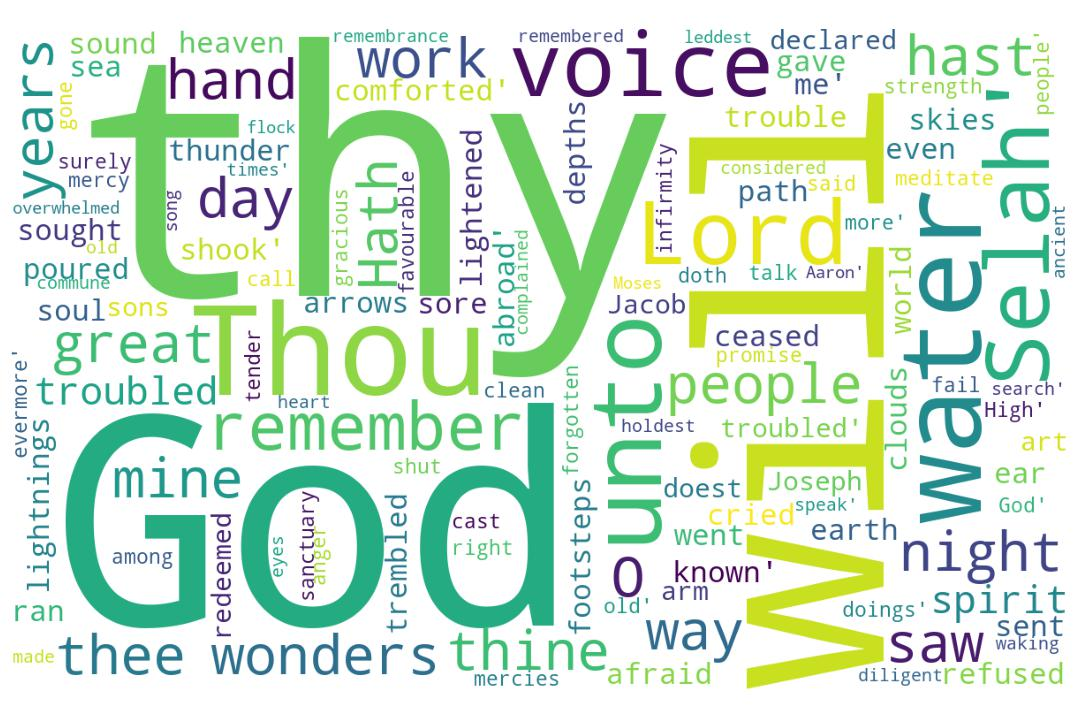
\includegraphics[width=\linewidth]{19OT-Psalms/Psalm77-WordCloud.jpg}
  \caption{Psalm 77 Word Cloud}
  \label{fig:Psalm 77 Word Cloud}
\end{figure}

\marginpar{\scriptsize \centering \fcolorbox{bone}{lime}{\textbf{GOD IS $\hdots$}}\\ (Psalm 77) \begin{compactenum}[I.][8]
    \item \textbf{My Silence} \index[scripture]{Psalms!Psa 077:04}(Psa 77:4)
    \item \textbf{My Searching} \index[scripture]{Psalms!Psa 077:06}(Psa 77:6)
    \item \textbf{My Song} \index[scripture]{Psalms!Psa 077:06}(Psa 77:6)
    \item \textbf{My Spech} \index[scripture]{Psalms!Psa 077:12}(Psa 77:12)
    \item \textbf{My Strength} \index[scripture]{Psalms!Psa 077:14}(Psa 77:14)
    \item \textbf{My Salvation} \index[scripture]{Psalms!Psa 077:15}(Psa 77:15)
    \item \textbf{My Saviour} \index[scripture]{Psalms!Psa 077:20}(Psa 77:20)
\end{compactenum}}
    

\marginpar{\scriptsize \centering \fcolorbox{bone}{yellow}{\textbf{A CHANGE OF}}\\
\fcolorbox{bone}{yellow}{\textbf{HEART AND MIND}}\\ (Psalm 77) 
\begin{compactenum}[I.][8]
    \item \textbf{There is Complaining} \index[scripture]{Psalms!Psa 077:03}(Psa 77:3)
    \item \textbf{There is Considering} \index[scripture]{Psalms!Psa 077:05}(Psa 77:5)
    \item \textbf{There is Communing with your Heart} \index[scripture]{Psalms!Psa 077:06}(Psa 77:6)
    \item \textbf{Thinking God Could Cast off his People} \index[scripture]{Psalms!Psa 077:07}(Psa 77:7)
    \item \textbf{But then Calling to Mind (remembering)} \index[scripture]{Psalms!Psa 077:11}(Psa 77:11)
    \item \textbf{And then God Confounds us} \index[scripture]{Psalms!Psa 077:13}(Psa 77:13) with his greatness, goodness, grace ...
    \item \textbf{That we can barely Contemplate Him} \index[scripture]{Psalms!Psa 077:14}(Psa 77:14)
\end{compactenum}}

\marginpar{\scriptsize \centering \fcolorbox{bone}{black}{\textbf{\textcolor{white}{THE PATH TO}}}\\ \fcolorbox{bone}{black}{\textbf{\textcolor{white}{DELIVERANCE}}}\\(Psalm 77) \begin{compactenum}[I.][8]
    \item \textbf{Revulsion} \index[scripture]{Psalms!Psa 077:02}(Psa 77:2)
    \item \textbf{Refusal} \index[scripture]{Psalms!Psa 077:03}(Psa 77:3)
    \item \textbf{Remembering} \index[scripture]{Psalms!Psa 077:03}\index[scripture]{Psalms!Psa 077:06}\index[scripture]{Psalms!Psa 077:11}\index[scripture]{Psalms!Psa 077:06}(Psa 77:3, 6, 10, 11)
    \item \textbf{Result} \index[scripture]{Psalms!Psa 077:10}(Psa 77:10)
    \item \textbf{Realization} \index[scripture]{Psalms!Psa 077:10}\index[scripture]{Psalms!Psa 077:13}(Psa 77:10, 13)
    \item \textbf{Redemption} \index[scripture]{Psalms!Psa 077:15}(Psa 77:15)
    \item \textbf{Revelation} \index[scripture]{Psalms!Psa 077:18}(Psa 77:18)
    \item \textbf{Rescue} \index[scripture]{Psalms!Psa 077:20}(Psa 77:20)
\end{compactenum}}


% \textcolor[cmyk]{0.99998,1,0,0}{
\footnote{\textcolor[rgb]{0.00,0.25,0.00}{\hyperlink{TOC}{Return to end of Table of Contents.}}}\footnote{\href{https://audiobible.com/bible/psalms_77.html}{\textcolor[cmyk]{0.99998,1,0,0}{Psalm 77 Audio}}}\textcolor[cmyk]{0.99998,1,0,0}{To the chief Musician, to Jeduthun, A Psalm of Asaph.}\\
\\
\textcolor[cmyk]{0.99998,1,0,0}{\fcolorbox{bone}{bone}{I} cried unto God with my voice, \emph{even} unto God with my voice; and he gave ear unto me.}
[2] \textcolor[cmyk]{0.99998,1,0,0}{In the day of my trouble \fcolorbox{bone}{bone}{I} sought the Lord: my sore ran in the night, and ceased not: my soul refused to be comforted.}\footnote{\textbf{Psalm 38:7} - For my loins are filled with a loathsome disease: and there is no soundness in my flesh.}
[3] \textcolor[cmyk]{0.99998,1,0,0}{\fcolorbox{bone}{bone}{I} remembered God, and was troubled: \fcolorbox{bone}{bone}{I} complained, and my spirit was overwhelmed. \fcolorbox{bone}{red}{\textcolor{white}{Selah}}.}
[4] \textcolor[cmyk]{0.99998,1,0,0}{Thou holdest mine eyes waking: \fcolorbox{bone}{bone}{I} am so troubled that \fcolorbox{bone}{bone}{I} cannot speak.}
[5] \textcolor[cmyk]{0.99998,1,0,0}{\fcolorbox{bone}{bone}{I} have considered the days of old, the years of ancient times.}\footnote{\textbf{Isaiah 46:10} - Declaring the end from the beginning, and from ancient times the things that are not yet done, saying, My counsel shall stand, and I will do all my pleasure:}
[6] \textcolor[cmyk]{0.99998,1,0,0}{\fcolorbox{bone}{bone}{I} call to remembrance my song in the night: \fcolorbox{bone}{bone}{I} commune with mine own heart: and my spirit made diligent search.}
[7] \textcolor[cmyk]{0.99998,1,0,0}{Will the Lord cast off for ever? and will he be favourable no more?}
[8] \textcolor[cmyk]{0.99998,1,0,0}{Is his mercy clean gone for ever? doth \emph{his} promise fail for evermore?}\footnote{\textbf{1 Kings 8:56} - Blessed be the LORD, that hath given rest unto his people Israel, according to all that he promised: there hath not failed one word of all his good promise, which he promised by the hand of Moses his servant.}
[9] \textcolor[cmyk]{0.99998,1,0,0}{Hath God forgotten to be gracious? hath he in anger shut up his tender mercies? \fcolorbox{bone}{red}{\textcolor{white}{Selah}}.}
[10] \textcolor[cmyk]{0.99998,1,0,0}{And \fcolorbox{bone}{bone}{I} said, This \emph{is} my infirmity: \emph{but} \emph{I} \emph{will} \emph{remember} the years of the right hand of the most High.}
[11] \textcolor[cmyk]{0.99998,1,0,0}{\fcolorbox{bone}{bone}{I} will remember the works of the LORD: surely \fcolorbox{bone}{bone}{I} will remember thy wonders of old.}
[12] \textcolor[cmyk]{0.99998,1,0,0}{\fcolorbox{bone}{bone}{I} will meditate also of all thy work, and talk of thy doings.}
[13] \textcolor[cmyk]{0.99998,1,0,0}{Thy way, O God, \emph{is} in the sanctuary: who \emph{is} \emph{so} great a God as \emph{our} God?}
[14] \textcolor[cmyk]{0.99998,1,0,0}{Thou \emph{art} the God that doest wonders: thou hast declared thy strength among the people.}
[15] \textcolor[cmyk]{0.99998,1,0,0}{Thou hast with \emph{thine} arm redeemed thy people, the sons of Jacob and Joseph. \fcolorbox{bone}{red}{\textcolor{white}{Selah}}.}
[16] \textcolor[cmyk]{0.99998,1,0,0}{The waters saw thee, O God, the waters saw thee; they were afraid: the depths also were troubled.}\footnote{\textbf{Job 41:32-32} - He maketh the deep to boil like a pot: he maketh the sea like a pot of ointment. [32] He maketh a path to shine after him; one would think the deep to be hoary. }\footnote{\textbf{Psalm 68:22} - The Lord said, I will bring again from Bashan, I will bring my people again from the depths of the sea:}
[17] \textcolor[cmyk]{0.99998,1,0,0}{The clouds poured out water: the skies sent out a sound: thine arrows also went abroad.}\footnote{\textbf{Psalm 18:14} - Yea, he sent out his arrows, and scattered them; and he shot out lightnings, and discomfited them.}\footnote{\textbf{Habakkuk 3:11} - The sun and moon stood still in their habitation: at the light of thine arrows they went, and at the shining of thy glittering spear}
[18] \textcolor[cmyk]{0.99998,1,0,0}{The voice of thy thunder \emph{was} in the heaven: the lightnings lightened the world: the earth trembled and shook.}
[19] \textcolor[cmyk]{0.99998,1,0,0}{Thy way \emph{is} in the sea, and thy path in the great waters, and thy footsteps are not known.}
[20] \textcolor[cmyk]{0.99998,1,0,0}{Thou leddest thy people like a flock by the hand of Moses and Aaron.}

\section{Psalm 77 Comments}

\subsection{Numeric Nuggets}
Verses 4, 8, and 12 have 13 words. Verses 1 and 16 have 13 unique words. The word ``I'' is used 13 times in the chapter (the word ``I'' in italics is found once). The 13$^{th}$ word in the chapter is the word ``voice'' (it is also the 7$^{th}$ word). The use of the word ``I'' ceases in verse 12. Verse 13 seems to be a transition verse: it has 13 words that are not italic! Verse 13 contains the word \emph{our} indicating the psalmist's recognition and acceptance of his place among God's redeemed people, Israel. The psalmist sends out six questions in verses 7-9, before the second ``Selah'' in verse 9 (the other two are in verses 3 and 15). Three ``Selahs'' are likely quite significant and likely have something to do with specific dealings of the LORD with Tribulation Israel.

\subsection{Psalm 77 Introduction}
The doctrinal content of this psalm is the Second Advent of Jesus Christ and his rescue of his people Israel. Spiritually, a sinner must recognize his desperate, deplorable, and hopeless condition before he will cry out to God for salvation. 

\subsection{Psalm 77:1}
Jeremiah 51:16 connects the ``voice'' with lightnings (as seen in verse 18).\footnote{\textbf{Jeremiah 51:16} - When he uttereth his voice, there is a multitude of waters in the heavens; and he causeth the vapours to ascend from the ends of the earth: he maketh lightnings with rain, and bringeth forth the wind out of his treasures.}

\subsection{Psalm 77:2}
This ``sore'' is the loathsome disease spoken of in Psalm 38:7.
\begin{center}

\begin{table}[ht]
\centering
\begin{tabular}{|p{.5in}|p{3.5in}|}
\hline

\textcolor[rgb]{0.00,0.00,1.00}{AV} & \textcolor[rgb]{0.00,0.00,1.00}{In the day of my trouble I sought the Lord: my sore ran in the night, and ceased not: my soul refused to be comforted.} \\ \hline 

\hline
\hline


ASV &  In the day of my trouble I sought the Lord: My hand was stretched out in the night, and slacked not; My soul refused to be comforted. \\ \hline
%
CEB &  During the day when I’m in trouble I look for my Lord.  At night my hands are still outstretched and don’t grow numb;  my whole being refuses to be comforted.\\ \hline
%
ESV & During the day when I’m in trouble I look for my Lord.  At night my hands are still outstretched and don’t grow numb;   my whole being[a] refuses to be comforted. \\ \hline
%
NASV & During the day when I’m in trouble I look for my Lord.  At night my hands are still outstretched and don’t grow numb;  my whole being[a] refuses to be comforted. \\ \hline
%
MEV & In the day of my trouble I sought the Lord;   in the night my hand is stretched out and does not weary,   my soul refuses to be comforted. \\ \hline
%
NIV &  In the day of my trouble I sought the Lord;  in the night my hand is stretched out and does not weary,   my soul refuses to be comforted. \\ \hline
%
NKJV &  In the day of my trouble I sought the Lord; in the night my hand is stretched out and does not weary,   my soul refuses to be comforted.\\ \hline
%
RSV &  In the day of my trouble I seek the Lord;  in the night my hand is stretched out without wearying;  my soul refuses to be comforted. \\ \hline

\hline
\hline

\multicolumn{2}{|p{4.3in}|}{{\textcolor{jungle}{Modern translations remove the reference to David's sore, his loathsome disease also seen in Psalm 38:7.  The versions spiritualize the phrase.  Leaving the text as it stands, we have an “issue of blood” (Lev. 12:7) or pus (Lev. 15:2) that will not dry up. It is a dripping infection coming from a limb; in this case, probably from the hands. \cite{Ruckman1992PsalmsV2}}}} \\ \hline

\end{tabular}
\caption[Corruption Alert: Psalm 77:2]{Corruption Alert: Psalm 77:2} \label{table:Corruption Psalm 77:2}

\end{table}

\end{center}




\subsection{Psalm 77:6}
Compare this ``diligent search'' with the diligent search carried out by the wicked.\footnote{\textbf{Psalm 64:6} - They search out iniquities; they accomplish a diligent search: both the inward thought of every one of them, and the heart, is deep. }

\subsection{Psalm 77:7-9}
The psalmist poses six questions:
\begin{compactenum}
    \item Will the Lord cast off for ever?
    \item Will he be favourable no more?
    \item Is his mercy clean gone for ever?
    \item Doth his promise fail for evermore?
    \item Hath God forgotten to be gracious 
    \item Hath he in anger shut up his tender mercies?\\
\end{compactenum}

\subsection{Psalm 77:10}
Note the mention of body, soul, and spirit in verses 2 and 3.
\begin{center}

\begin{table}[ht]
\centering
\begin{tabular}{|p{.5in}|p{3.5in}|}
\hline

\textcolor[rgb]{0.00,0.00,1.00}{AV} & \textcolor[rgb]{0.00,0.00,1.00}{And I said, This \emph{is} my infirmity: \emph{but} \emph{I} \emph{will} \emph{remember} the years of the right hand of the most High.} \\ \hline 

\hline
\hline


ASV &  And I said, This is my infirmity; But I will remember the years of the right hand of the Most High. \\ \hline
%
CEB &  It’s my misfortune, I thought,  that the strong hand of the Most High is different now.\\ \hline
%
ESV & TThen I said, ``I will appeal to this, to the years of the right hand of the Most High.'' \\ \hline
%
NASV &  Then I said, “It is my grief, That the right hand of the Most High has changed.” \\ \hline
%
MEV & Then I said, “This is my grief;  yet I will remember the years of the right hand of the Most High.” \\ \hline
%
NIV &  Then I thought, “To this I will appeal:  the years when the Most High stretched out his right hand. \\ \hline
%
NKJV &  And I said, “This is my anguish;
But I will remember the years of the right hand of the Most High.”\\ \hline
%
RSV &  And I say, “It is my grief that the right hand of the Most High has changed.”. \\ \hline

\hline
\hline

\multicolumn{2}{|p{4.3in}|}{{\textcolor{jungle}{The word ``infirmity'' is changed to “anguish,” “grief,” and “misfortune.” It is removed completely in the ESV and NIV. The effect is destroying the connection to “sore” in verse 2. The psalmist here, who typifies the Tribulation Jew, has 2 infirmities: A physical one, and a spiritual one. The infirmity, or infirmities, are emphasized by the word ``my.'' Ruckman points out that and infirmity is a weakness as in 2 Corinthians 11:30 and 12:5.\cite{Ruckman1992PsalmsV2}.}}} \\ \hline

\end{tabular}
\caption[Corruption Alert: Psalm 77:10]{Corruption Alert: Psalm 77:10} \label{table:Corruption Psalm 77:10}

\end{table}

\end{center}




\noindent The answer (to the six questions), in general, with respect to Israel, is a resounding ``No!'' The mercies are called for by David in 2 Samuel 24:14 and 1 Chronicles 21:13.\footnote{\textbf{2 Samuel 24:14} - And David said unto Gad, I am in a great strait: let us fall now into the hand of the LORD; for his mercies are great: and let me not fall into the hand of man.}\footnote{\textbf{1 Chronicles 21:13} - And David said unto Gad, I am in a great strait: let me fall now into the hand of the LORD; for very great are his mercies: but let me not fall into the hand of man.}\cite{Ruckman1992PsalmsV2}

\subsection{Psalm 77:9}
The phrase ``tender mercies'' shows up eleven times in scripture, ten occurrences of which speak of the Lord's ``tender mercies.'' All of these are in Psalms (Psalms 25:6, 40:11, 51:1, 69:16, 77:9, 79:8, 103:4, 119:77, 119:156, and  145:9.) Number eleven describes the ``tender mercies'' of the wicked, called cruel. So, question number six is answered (confirmed in Lamentations 3:22). \footnote{\textbf{Lamentations 3:22} - It is of the LORD’S mercies that we are not consumed, because his compassions fail not.} But, in Jeremiah 16:5, they are temporarily taken away.\footnote{\textbf{Jeremiah 16:5} - For thus saith the LORD, Enter not into the house of mourning, neither go to lament nor bemoan them: for I have taken away my peace from this people, saith the LORD, even lovingkindness and mercies.}\cite{Ruckman1992PsalmsV2}

\subsection{Psalm 77:17-19}
Psalm 18 is a wonderful parallel passage to Psalm 77. Verse 14 speaks of God's arrows and lightnings. It also speaks of the ``channels'' of waters spoke of here in verse 18. This ``path in the great waters'' is the route the LORD will take with his armies for is return at the Second Advent.\footnote{\textbf{PSalm 18} - I will love thee, O LORD, my strength. [2] The LORD is my rock, and my fortress, and my deliverer; my God, my strength, in whom I will trust; my buckler, and the horn of my salvation, and my high tower. [3] I will call upon the LORD, who is worthy to be praised: so shall I be saved from mine enemies. [4] The sorrows of death compassed me, and the floods of ungodly men made me afraid. [5] The sorrows of hell compassed me about: the snares of death prevented me. [6] In my distress I called upon the LORD, and cried unto my God: he heard my voice out of his temple, and my cry came before him, even into his ears. [7] Then the earth shook and trembled; the foundations also of the hills moved and were shaken, because he was wroth. [8] There went up a smoke out of his nostrils, and fire out of his mouth devoured: coals were kindled by it. [9] He bowed the heavens also, and came down: and darkness was under his feet. [10] And he rode upon a cherub, and did fly: yea, he did fly upon the wings of the wind. [11] He made darkness his secret place; his pavilion round about him were dark waters and thick clouds of the skies. [12] At the brightness that was before him his thick clouds passed, hail stones and coals of fire. [13] The LORD also thundered in the heavens, and the Highest gave his voice; hail stones and coals of fire. [14] Yea, he sent out his arrows, and scattered them; and he shot out lightnings, and discomfited them. [15] Then the channels of waters were seen, and the foundations of the world were discovered at thy rebuke, O LORD, at the blast of the breath of thy nostrils. [16] He sent from above, he took me, he drew me out of many waters. [17] He delivered me from my strong enemy, and from them which hated me: for they were too strong for me. [18] They prevented me in the day of my calamity: but the LORD was my stay. [19] He brought me forth also into a large place; he delivered me, because he delighted in me. [20] The LORD rewarded me according to my righteousness; according to the cleanness of my hands hath he recompensed me. [21] For I have kept the ways of the LORD, and have not wickedly departed from my God. [22] For all his judgments were before me, and I did not put away his statutes from me. [23] I was also upright before him, and I kept myself from mine iniquity. [24] Therefore hath the LORD recompensed me according to my righteousness, according to the cleanness of my hands in his eyesight. [25] With the merciful thou wilt shew thyself merciful; with an upright man thou wilt shew thyself upright; [26] With the pure thou wilt shew thyself pure; and with the froward thou wilt shew thyself froward. [27] For thou wilt save the afflicted people; but wilt bring down high looks. [28] For thou wilt light my candle: the LORD my God will enlighten my darkness. [29] For by thee I have run through a troop; and by my God have I leaped over a wall. [30] As for God, his way is perfect: the word of the LORD is tried: he is a buckler to all those that trust in him. [31] For who is God save the LORD? or who is a rock save our God? [32] It is God that girdeth me with strength, and maketh my way perfect. [33] He maketh my feet like hinds’ feet, and setteth me upon my high places. [34] He teacheth my hands to war, so that a bow of steel is broken by mine arms. [35] Thou hast also given me the shield of thy salvation: and thy right hand hath holden me up, and thy gentleness hath made me great. [36] Thou hast enlarged my steps under me, that my feet did not slip. [37] I have pursued mine enemies, and overtaken them: neither did I turn again till they were consumed. [38] I have wounded them that they were not able to rise: they are fallen under my feet. [39] For thou hast girded me with strength unto the battle: thou hast subdued under me those that rose up against me. [40] Thou hast also given me the necks of mine enemies; that I might destroy them that hate me. [41] They cried, but there was none to save them: even unto the LORD, but he answered them not. [42] Then did I beat them small as the dust before the wind: I did cast them out as the dirt in the streets. [43] Thou hast delivered me from the strivings of the people; and thou hast made me the head of the heathen: a people whom I have not known shall serve me. [44] As soon as they hear of me, they shall obey me: the strangers shall submit themselves unto me. [45] The strangers shall fade away, and be afraid out of their close places. [46] The LORD liveth; and blessed be my rock; and let the God of my salvation be exalted. [47] It is God that avengeth me, and subdueth the people under me. [48] He delivereth me from mine enemies: yea, thou liftest me up above those that rise up against me: thou hast delivered me from the violent man. [49] Therefore will I give thanks unto thee, O LORD, among the heathen, and sing praises unto thy name. [50] Great deliverance giveth he to his king; and sheweth mercy to his anointed, to David, and to his seed for evermore.}\cite{Ruckman1992PsalmsV2}

\subsection{Psalm 77:20}
Another comparison is the in Numbers 33:1.\footnote{\textbf{Numbers 33:1} - These are the journeys of the children of Israel, which went forth out of the land of Egypt with their armies under the hand of Moses and Aaron.}\cite{Ruckman1992PsalmsV2}


%\index[NWIV]{19!Psalms!Psa 77:1}\index[AWIP]{I!Psalms!Psa 77:1}\index[AWIP]{cried!Psalms!Psa 77:1}\index[AWIP]{unto!Psalms!Psa 77:1}\index[AWIP]{unto!Psalms!Psa 77:1 (2)}\index[AWIP]{unto!Psalms!Psa 77:1 (3)}\index[AWIP]{God!Psalms!Psa 77:1}\index[AWIP]{God!Psalms!Psa 77:1 (2)}\index[AWIP]{with!Psalms!Psa 77:1}\index[AWIP]{with!Psalms!Psa 77:1 (2)}\index[AWIP]{my!Psalms!Psa 77:1}\index[AWIP]{my!Psalms!Psa 77:1 (2)}\index[AWIP]{voice!Psalms!Psa 77:1}\index[AWIP]{voice!Psalms!Psa 77:1 (2)}\index[AWIP]{\emph{even}!Psalms!Psa 77:1}\index[AWIP]{and!Psalms!Psa 77:1}\index[AWIP]{he!Psalms!Psa 77:1}\index[AWIP]{gave!Psalms!Psa 77:1}\index[AWIP]{ear!Psalms!Psa 77:1}\index[AWIP]{me!Psalms!Psa 77:1}\index[AWIP]{\emph{even}!Psalms!Psa 77:1}

\index[NWIV]{25!Psalms!Psa 77:2}\index[AWIP]{In!Psalms!Psa 77:2}\index[AWIP]{the!Psalms!Psa 77:2}\index[AWIP]{the!Psalms!Psa 77:2 (2)}\index[AWIP]{the!Psalms!Psa 77:2 (3)}\index[AWIP]{day!Psalms!Psa 77:2}\index[AWIP]{of!Psalms!Psa 77:2}\index[AWIP]{my!Psalms!Psa 77:2}\index[AWIP]{my!Psalms!Psa 77:2 (2)}\index[AWIP]{my!Psalms!Psa 77:2 (3)}\index[AWIP]{trouble!Psalms!Psa 77:2}\index[AWIP]{I!Psalms!Psa 77:2}\index[AWIP]{sought!Psalms!Psa 77:2}\index[AWIP]{Lord!Psalms!Psa 77:2}\index[AWIP]{sore!Psalms!Psa 77:2}\index[AWIP]{ran!Psalms!Psa 77:2}\index[AWIP]{in!Psalms!Psa 77:2}\index[AWIP]{night!Psalms!Psa 77:2}\index[AWIP]{and!Psalms!Psa 77:2}\index[AWIP]{ceased!Psalms!Psa 77:2}\index[AWIP]{not!Psalms!Psa 77:2}\index[AWIP]{soul!Psalms!Psa 77:2}\index[AWIP]{refused!Psalms!Psa 77:2}\index[AWIP]{to!Psalms!Psa 77:2}\index[AWIP]{be!Psalms!Psa 77:2}\index[AWIP]{comforted!Psalms!Psa 77:2}

\index[NWIV]{14!Psalms!Psa 77:3}\index[AWIP]{I!Psalms!Psa 77:3}\index[AWIP]{I!Psalms!Psa 77:3 (2)}\index[AWIP]{remembered!Psalms!Psa 77:3}\index[AWIP]{God!Psalms!Psa 77:3}\index[AWIP]{and!Psalms!Psa 77:3}\index[AWIP]{and!Psalms!Psa 77:3 (2)}\index[AWIP]{was!Psalms!Psa 77:3}\index[AWIP]{was!Psalms!Psa 77:3 (2)}\index[AWIP]{troubled!Psalms!Psa 77:3}\index[AWIP]{complained!Psalms!Psa 77:3}\index[AWIP]{my!Psalms!Psa 77:3}\index[AWIP]{spirit!Psalms!Psa 77:3}\index[AWIP]{overwhelmed!Psalms!Psa 77:3}\index[AWIP]{Selah!Psalms!Psa 77:3}

\index[NWIV]{13!Psalms!Psa 77:4}\index[AWIP]{Thou!Psalms!Psa 77:4}\index[AWIP]{holdest!Psalms!Psa 77:4}\index[AWIP]{mine!Psalms!Psa 77:4}\index[AWIP]{eyes!Psalms!Psa 77:4}\index[AWIP]{waking!Psalms!Psa 77:4}\index[AWIP]{I!Psalms!Psa 77:4}\index[AWIP]{I!Psalms!Psa 77:4 (2)}\index[AWIP]{am!Psalms!Psa 77:4}\index[AWIP]{so!Psalms!Psa 77:4}\index[AWIP]{troubled!Psalms!Psa 77:4}\index[AWIP]{that!Psalms!Psa 77:4}\index[AWIP]{cannot!Psalms!Psa 77:4}\index[AWIP]{speak!Psalms!Psa 77:4}

\index[NWIV]{12!Psalms!Psa 77:5}\index[AWIP]{I!Psalms!Psa 77:5}\index[AWIP]{have!Psalms!Psa 77:5}\index[AWIP]{considered!Psalms!Psa 77:5}\index[AWIP]{the!Psalms!Psa 77:5}\index[AWIP]{the!Psalms!Psa 77:5 (2)}\index[AWIP]{days!Psalms!Psa 77:5}\index[AWIP]{of!Psalms!Psa 77:5}\index[AWIP]{of!Psalms!Psa 77:5 (2)}\index[AWIP]{old!Psalms!Psa 77:5}\index[AWIP]{years!Psalms!Psa 77:5}\index[AWIP]{ancient!Psalms!Psa 77:5}\index[AWIP]{times!Psalms!Psa 77:5}

\index[NWIV]{21!Psalms!Psa 77:6}\index[AWIP]{I!Psalms!Psa 77:6}\index[AWIP]{I!Psalms!Psa 77:6 (2)}\index[AWIP]{call!Psalms!Psa 77:6}\index[AWIP]{to!Psalms!Psa 77:6}\index[AWIP]{remembrance!Psalms!Psa 77:6}\index[AWIP]{my!Psalms!Psa 77:6}\index[AWIP]{my!Psalms!Psa 77:6 (2)}\index[AWIP]{song!Psalms!Psa 77:6}\index[AWIP]{in!Psalms!Psa 77:6}\index[AWIP]{the!Psalms!Psa 77:6}\index[AWIP]{night!Psalms!Psa 77:6}\index[AWIP]{commune!Psalms!Psa 77:6}\index[AWIP]{with!Psalms!Psa 77:6}\index[AWIP]{mine!Psalms!Psa 77:6}\index[AWIP]{own!Psalms!Psa 77:6}\index[AWIP]{heart!Psalms!Psa 77:6}\index[AWIP]{and!Psalms!Psa 77:6}\index[AWIP]{spirit!Psalms!Psa 77:6}\index[AWIP]{made!Psalms!Psa 77:6}\index[AWIP]{diligent!Psalms!Psa 77:6}\index[AWIP]{search!Psalms!Psa 77:6}

\index[NWIV]{14!Psalms!Psa 77:7}\index[AWIP]{Will!Psalms!Psa 77:7}\index[AWIP]{the!Psalms!Psa 77:7}\index[AWIP]{Lord!Psalms!Psa 77:7}\index[AWIP]{cast!Psalms!Psa 77:7}\index[AWIP]{off!Psalms!Psa 77:7}\index[AWIP]{for!Psalms!Psa 77:7}\index[AWIP]{ever?!Psalms!Psa 77:7}\index[AWIP]{and!Psalms!Psa 77:7}\index[AWIP]{will!Psalms!Psa 77:7}\index[AWIP]{he!Psalms!Psa 77:7}\index[AWIP]{be!Psalms!Psa 77:7}\index[AWIP]{favourable!Psalms!Psa 77:7}\index[AWIP]{no!Psalms!Psa 77:7}\index[AWIP]{more?!Psalms!Psa 77:7}

\index[NWIV]{13!Psalms!Psa 77:8}\index[AWIP]{Is!Psalms!Psa 77:8}\index[AWIP]{his!Psalms!Psa 77:8}\index[AWIP]{mercy!Psalms!Psa 77:8}\index[AWIP]{clean!Psalms!Psa 77:8}\index[AWIP]{gone!Psalms!Psa 77:8}\index[AWIP]{for!Psalms!Psa 77:8}\index[AWIP]{for!Psalms!Psa 77:8 (2)}\index[AWIP]{ever?!Psalms!Psa 77:8}\index[AWIP]{doth!Psalms!Psa 77:8}\index[AWIP]{\emph{his}!Psalms!Psa 77:8}\index[AWIP]{promise!Psalms!Psa 77:8}\index[AWIP]{fail!Psalms!Psa 77:8}\index[AWIP]{evermore?!Psalms!Psa 77:8}\index[AWIP]{\emph{his}!Psalms!Psa 77:8}

\index[NWIV]{16!Psalms!Psa 77:9}\index[AWIP]{Hath!Psalms!Psa 77:9}\index[AWIP]{God!Psalms!Psa 77:9}\index[AWIP]{forgotten!Psalms!Psa 77:9}\index[AWIP]{to!Psalms!Psa 77:9}\index[AWIP]{be!Psalms!Psa 77:9}\index[AWIP]{gracious?!Psalms!Psa 77:9}\index[AWIP]{hath!Psalms!Psa 77:9}\index[AWIP]{he!Psalms!Psa 77:9}\index[AWIP]{in!Psalms!Psa 77:9}\index[AWIP]{anger!Psalms!Psa 77:9}\index[AWIP]{shut!Psalms!Psa 77:9}\index[AWIP]{up!Psalms!Psa 77:9}\index[AWIP]{his!Psalms!Psa 77:9}\index[AWIP]{tender!Psalms!Psa 77:9}\index[AWIP]{mercies?!Psalms!Psa 77:9}\index[AWIP]{Selah!Psalms!Psa 77:9}

\index[NWIV]{21!Psalms!Psa 77:10}\index[AWIP]{And!Psalms!Psa 77:10}\index[AWIP]{I!Psalms!Psa 77:10}\index[AWIP]{said!Psalms!Psa 77:10}\index[AWIP]{This!Psalms!Psa 77:10}\index[AWIP]{\emph{is}!Psalms!Psa 77:10}\index[AWIP]{my!Psalms!Psa 77:10}\index[AWIP]{infirmity!Psalms!Psa 77:10}\index[AWIP]{\emph{but}!Psalms!Psa 77:10}\index[AWIP]{\emph{I}!Psalms!Psa 77:10}\index[AWIP]{\emph{will}!Psalms!Psa 77:10}\index[AWIP]{\emph{remember}!Psalms!Psa 77:10}\index[AWIP]{the!Psalms!Psa 77:10}\index[AWIP]{the!Psalms!Psa 77:10 (2)}\index[AWIP]{the!Psalms!Psa 77:10 (3)}\index[AWIP]{years!Psalms!Psa 77:10}\index[AWIP]{of!Psalms!Psa 77:10}\index[AWIP]{of!Psalms!Psa 77:10 (2)}\index[AWIP]{right!Psalms!Psa 77:10}\index[AWIP]{hand!Psalms!Psa 77:10}\index[AWIP]{most!Psalms!Psa 77:10}\index[AWIP]{High!Psalms!Psa 77:10}\index[AWIP]{\emph{is}!Psalms!Psa 77:10}\index[AWIP]{\emph{but}!Psalms!Psa 77:10}\index[AWIP]{\emph{I}!Psalms!Psa 77:10}\index[AWIP]{\emph{will}!Psalms!Psa 77:10}\index[AWIP]{\emph{remember}!Psalms!Psa 77:10}

\index[NWIV]{16!Psalms!Psa 77:11}\index[AWIP]{I!Psalms!Psa 77:11}\index[AWIP]{I!Psalms!Psa 77:11 (2)}\index[AWIP]{will!Psalms!Psa 77:11}\index[AWIP]{will!Psalms!Psa 77:11 (2)}\index[AWIP]{remember!Psalms!Psa 77:11}\index[AWIP]{remember!Psalms!Psa 77:11 (2)}\index[AWIP]{the!Psalms!Psa 77:11}\index[AWIP]{the!Psalms!Psa 77:11 (2)}\index[AWIP]{works!Psalms!Psa 77:11}\index[AWIP]{of!Psalms!Psa 77:11}\index[AWIP]{of!Psalms!Psa 77:11 (2)}\index[AWIP]{LORD!Psalms!Psa 77:11}\index[AWIP]{surely!Psalms!Psa 77:11}\index[AWIP]{thy!Psalms!Psa 77:11}\index[AWIP]{wonders!Psalms!Psa 77:11}\index[AWIP]{old!Psalms!Psa 77:11}

\index[NWIV]{13!Psalms!Psa 77:12}\index[AWIP]{I!Psalms!Psa 77:12}\index[AWIP]{will!Psalms!Psa 77:12}\index[AWIP]{meditate!Psalms!Psa 77:12}\index[AWIP]{also!Psalms!Psa 77:12}\index[AWIP]{of!Psalms!Psa 77:12}\index[AWIP]{of!Psalms!Psa 77:12 (2)}\index[AWIP]{all!Psalms!Psa 77:12}\index[AWIP]{thy!Psalms!Psa 77:12}\index[AWIP]{thy!Psalms!Psa 77:12 (2)}\index[AWIP]{work!Psalms!Psa 77:12}\index[AWIP]{and!Psalms!Psa 77:12}\index[AWIP]{talk!Psalms!Psa 77:12}\index[AWIP]{doings!Psalms!Psa 77:12}

\index[NWIV]{17!Psalms!Psa 77:13}\index[AWIP]{Thy!Psalms!Psa 77:13}\index[AWIP]{way!Psalms!Psa 77:13}\index[AWIP]{O!Psalms!Psa 77:13}\index[AWIP]{God!Psalms!Psa 77:13}\index[AWIP]{God!Psalms!Psa 77:13 (2)}\index[AWIP]{\emph{is}!Psalms!Psa 77:13}\index[AWIP]{\emph{is}!Psalms!Psa 77:13 (2)}\index[AWIP]{in!Psalms!Psa 77:13}\index[AWIP]{the!Psalms!Psa 77:13}\index[AWIP]{sanctuary!Psalms!Psa 77:13}\index[AWIP]{who!Psalms!Psa 77:13}\index[AWIP]{\emph{so}!Psalms!Psa 77:13}\index[AWIP]{great!Psalms!Psa 77:13}\index[AWIP]{a!Psalms!Psa 77:13}\index[AWIP]{as!Psalms!Psa 77:13}\index[AWIP]{\emph{our}!Psalms!Psa 77:13}\index[AWIP]{God?!Psalms!Psa 77:13}\index[AWIP]{\emph{is}!Psalms!Psa 77:13}\index[AWIP]{\emph{is}!Psalms!Psa 77:13 (2)}\index[AWIP]{\emph{so}!Psalms!Psa 77:13}\index[AWIP]{\emph{our}!Psalms!Psa 77:13}

\index[NWIV]{15!Psalms!Psa 77:14}\index[AWIP]{Thou!Psalms!Psa 77:14}\index[AWIP]{\emph{art}!Psalms!Psa 77:14}\index[AWIP]{the!Psalms!Psa 77:14}\index[AWIP]{the!Psalms!Psa 77:14 (2)}\index[AWIP]{God!Psalms!Psa 77:14}\index[AWIP]{that!Psalms!Psa 77:14}\index[AWIP]{doest!Psalms!Psa 77:14}\index[AWIP]{wonders!Psalms!Psa 77:14}\index[AWIP]{thou!Psalms!Psa 77:14}\index[AWIP]{hast!Psalms!Psa 77:14}\index[AWIP]{declared!Psalms!Psa 77:14}\index[AWIP]{thy!Psalms!Psa 77:14}\index[AWIP]{strength!Psalms!Psa 77:14}\index[AWIP]{among!Psalms!Psa 77:14}\index[AWIP]{people!Psalms!Psa 77:14}\index[AWIP]{\emph{art}!Psalms!Psa 77:14}

\index[NWIV]{15!Psalms!Psa 77:15}\index[AWIP]{Thou!Psalms!Psa 77:15}\index[AWIP]{hast!Psalms!Psa 77:15}\index[AWIP]{with!Psalms!Psa 77:15}\index[AWIP]{\emph{thine}!Psalms!Psa 77:15}\index[AWIP]{arm!Psalms!Psa 77:15}\index[AWIP]{redeemed!Psalms!Psa 77:15}\index[AWIP]{thy!Psalms!Psa 77:15}\index[AWIP]{people!Psalms!Psa 77:15}\index[AWIP]{the!Psalms!Psa 77:15}\index[AWIP]{sons!Psalms!Psa 77:15}\index[AWIP]{of!Psalms!Psa 77:15}\index[AWIP]{Jacob!Psalms!Psa 77:15}\index[AWIP]{and!Psalms!Psa 77:15}\index[AWIP]{Joseph!Psalms!Psa 77:15}\index[AWIP]{Selah!Psalms!Psa 77:15}\index[AWIP]{\emph{thine}!Psalms!Psa 77:15}

\index[NWIV]{18!Psalms!Psa 77:16}\index[AWIP]{The!Psalms!Psa 77:16}\index[AWIP]{waters!Psalms!Psa 77:16}\index[AWIP]{waters!Psalms!Psa 77:16 (2)}\index[AWIP]{saw!Psalms!Psa 77:16}\index[AWIP]{saw!Psalms!Psa 77:16 (2)}\index[AWIP]{thee!Psalms!Psa 77:16}\index[AWIP]{thee!Psalms!Psa 77:16 (2)}\index[AWIP]{O!Psalms!Psa 77:16}\index[AWIP]{God!Psalms!Psa 77:16}\index[AWIP]{the!Psalms!Psa 77:16}\index[AWIP]{the!Psalms!Psa 77:16 (2)}\index[AWIP]{they!Psalms!Psa 77:16}\index[AWIP]{were!Psalms!Psa 77:16}\index[AWIP]{were!Psalms!Psa 77:16 (2)}\index[AWIP]{afraid!Psalms!Psa 77:16}\index[AWIP]{depths!Psalms!Psa 77:16}\index[AWIP]{also!Psalms!Psa 77:16}\index[AWIP]{troubled!Psalms!Psa 77:16}

\index[NWIV]{16!Psalms!Psa 77:17}\index[AWIP]{The!Psalms!Psa 77:17}\index[AWIP]{clouds!Psalms!Psa 77:17}\index[AWIP]{poured!Psalms!Psa 77:17}\index[AWIP]{out!Psalms!Psa 77:17}\index[AWIP]{out!Psalms!Psa 77:17 (2)}\index[AWIP]{water!Psalms!Psa 77:17}\index[AWIP]{the!Psalms!Psa 77:17}\index[AWIP]{skies!Psalms!Psa 77:17}\index[AWIP]{sent!Psalms!Psa 77:17}\index[AWIP]{a!Psalms!Psa 77:17}\index[AWIP]{sound!Psalms!Psa 77:17}\index[AWIP]{thine!Psalms!Psa 77:17}\index[AWIP]{arrows!Psalms!Psa 77:17}\index[AWIP]{also!Psalms!Psa 77:17}\index[AWIP]{went!Psalms!Psa 77:17}\index[AWIP]{abroad!Psalms!Psa 77:17}

\index[NWIV]{19!Psalms!Psa 77:18}\index[AWIP]{The!Psalms!Psa 77:18}\index[AWIP]{voice!Psalms!Psa 77:18}\index[AWIP]{of!Psalms!Psa 77:18}\index[AWIP]{thy!Psalms!Psa 77:18}\index[AWIP]{thunder!Psalms!Psa 77:18}\index[AWIP]{\emph{was}!Psalms!Psa 77:18}\index[AWIP]{in!Psalms!Psa 77:18}\index[AWIP]{the!Psalms!Psa 77:18}\index[AWIP]{the!Psalms!Psa 77:18 (2)}\index[AWIP]{the!Psalms!Psa 77:18 (3)}\index[AWIP]{the!Psalms!Psa 77:18 (4)}\index[AWIP]{heaven!Psalms!Psa 77:18}\index[AWIP]{lightnings!Psalms!Psa 77:18}\index[AWIP]{lightened!Psalms!Psa 77:18}\index[AWIP]{world!Psalms!Psa 77:18}\index[AWIP]{earth!Psalms!Psa 77:18}\index[AWIP]{trembled!Psalms!Psa 77:18}\index[AWIP]{and!Psalms!Psa 77:18}\index[AWIP]{shook!Psalms!Psa 77:18}\index[AWIP]{\emph{was}!Psalms!Psa 77:18}

\index[NWIV]{19!Psalms!Psa 77:19}\index[AWIP]{Thy!Psalms!Psa 77:19}\index[AWIP]{way!Psalms!Psa 77:19}\index[AWIP]{\emph{is}!Psalms!Psa 77:19}\index[AWIP]{in!Psalms!Psa 77:19}\index[AWIP]{in!Psalms!Psa 77:19 (2)}\index[AWIP]{the!Psalms!Psa 77:19}\index[AWIP]{the!Psalms!Psa 77:19 (2)}\index[AWIP]{sea!Psalms!Psa 77:19}\index[AWIP]{and!Psalms!Psa 77:19}\index[AWIP]{and!Psalms!Psa 77:19 (2)}\index[AWIP]{thy!Psalms!Psa 77:19}\index[AWIP]{thy!Psalms!Psa 77:19 (2)}\index[AWIP]{path!Psalms!Psa 77:19}\index[AWIP]{great!Psalms!Psa 77:19}\index[AWIP]{waters!Psalms!Psa 77:19}\index[AWIP]{footsteps!Psalms!Psa 77:19}\index[AWIP]{are!Psalms!Psa 77:19}\index[AWIP]{not!Psalms!Psa 77:19}\index[AWIP]{known!Psalms!Psa 77:19}\index[AWIP]{\emph{is}!Psalms!Psa 77:19}

\index[NWIV]{14!Psalms!Psa 77:20}\index[AWIP]{Thou!Psalms!Psa 77:20}\index[AWIP]{leddest!Psalms!Psa 77:20}\index[AWIP]{thy!Psalms!Psa 77:20}\index[AWIP]{people!Psalms!Psa 77:20}\index[AWIP]{like!Psalms!Psa 77:20}\index[AWIP]{a!Psalms!Psa 77:20}\index[AWIP]{flock!Psalms!Psa 77:20}\index[AWIP]{by!Psalms!Psa 77:20}\index[AWIP]{the!Psalms!Psa 77:20}\index[AWIP]{hand!Psalms!Psa 77:20}\index[AWIP]{of!Psalms!Psa 77:20}\index[AWIP]{Moses!Psalms!Psa 77:20}\index[AWIP]{and!Psalms!Psa 77:20}\index[AWIP]{Aaron!Psalms!Psa 77:20}


\section{Psalm 77 Outlines}

\subsection{My Outlines} 

\subsubsection{God Is ... }
\index[speaker]{Keith Anthony!Psalm 077 (God Is ...)}
\index[series]{Psalms (Keith Anthony)!Psalm 077 (God Is ...)}
\index[date]{2015/08/21!Psalm 077 (God Is ...) (Keith Anthony)}
\begin{compactenum}[I.]
    \item \textbf{My Silence} \index[scripture]{Psalms!Psa 077:04}(Psa 77:4)
    \item \textbf{My Searching} \index[scripture]{Psalms!Psa 077:06}(Psa 77:6)
    \item \textbf{My Song} \index[scripture]{Psalms!Psa 077:06}(Psa 77:6)
    \item \textbf{My Spech} \index[scripture]{Psalms!Psa 077:12}(Psa 77:12)
    \item \textbf{My Strength} \index[scripture]{Psalms!Psa 077:14}(Psa 77:14)
    \item \textbf{My Salvation} \index[scripture]{Psalms!Psa 077:15}(Psa 77:15)
    \item \textbf{My Saviour} \index[scripture]{Psalms!Psa 077:20}(Psa 77:20)
\end{compactenum}

\subsubsection{A Change of Heart and Mind}
\index[speaker]{Keith Anthony!Psalm 077 (A Change of Heart and Mind }
\index[series]{Psalms (Keith Anthony)!Psalm 077 (A Change of Heart and Mind}
\index[date]{2015/08/21!Psalm 077 (A Change of Heart and Mind) (Keith Anthony)}
\begin{compactenum}[I.]
    \item \textbf{There is Complaining} \index[scripture]{Psalms!Psa 077:03}(Psa 77:3)
    \item \textbf{There is Considering} \index[scripture]{Psalms!Psa 077:05}(Psa 77:5)
    \item \textbf{There is Communing with your Heart} \index[scripture]{Psalms!Psa 077:06}(Psa 77:6)
    \item \textbf{Thinking God Could Cast off his People} \index[scripture]{Psalms!Psa 077:07}(Psa 77:7)
    \item \textbf{But then Calling to Mind (remembering)} \index[scripture]{Psalms!Psa 077:11}(Psa 77:11)
    \item \textbf{And then God Confounds us} \index[scripture]{Psalms!Psa 077:13}(Psa 77:13) with his greatness, goodness, grace ...
    \item \textbf{That we can barely Contemplate Him} \index[scripture]{Psalms!Psa 077:14}(Psa 77:14)
\end{compactenum}

\subsubsection{The Path to Deliverance}
\index[speaker]{Keith Anthony!Psalm 077 (Israel's Path to Deliverance}
\index[series]{Psalms (Keith Anthony)!Psalm 077 (Israel's Path to Deliverance}
\index[date]{2021/09/05!Psalm 077 (Israel's Path to Deliverance) (Keith Anthony)}
\begin{compactenum}[I.][8]
    \item \textbf{Revulsion} \index[scripture]{Psalms!Psa 077:02}(Psa 77:2)
    \item \textbf{Refusal} \index[scripture]{Psalms!Psa 077:03}(Psa 77:3)
    \item \textbf{Remembering} \index[scripture]{Psalms!Psa 077:03}\index[scripture]{Psalms!Psa 077:06}\index[scripture]{Psalms!Psa 077:11}\index[scripture]{Psalms!Psa 077:06}(Psa 77:3, 6, 10, 11)
    \item \textbf{Result} \index[scripture]{Psalms!Psa 077:10}(Psa 77:10)
    \item \textbf{Realization} \index[scripture]{Psalms!Psa 077:10}\index[scripture]{Psalms!Psa 077:13}(Psa 77:10, 13)
    \item \textbf{Redemption} \index[scripture]{Psalms!Psa 077:15}(Psa 77:15)
    \item \textbf{Revelation} \index[scripture]{Psalms!Psa 077:18}(Psa 77:18)
    \item \textbf{Rescue} \index[scripture]{Psalms!Psa 077:20}(Psa 77:20)
\end{compactenum}


\section{Outlines from Others}

%\subsubsection{What to do when you start talking to yourself}
%\index[speaker]{Richard Drummond!Psalm 077 (What to do when you start talking to yourself}
%\index[series]{Psalms (Richard Drummond)!Psalm 077 (What to do when you start talking to yourself)}
%\index[date]{2014/05/25!Psalm 077 (What to do when you start talking to yourself)) (Richard Drummond)}
%\begin{compactenum}[I.][4]
%	\item Stop and \textbf{Remember} the years at the years of the right hand of God ... forget the past ...cannot change history \index[scripture]{Psalms!Psa 077:10}(Psalm 77:10)
%	\item \textbf{Remember} the works of the Lord \index[scripture]{Mathew!Matt 06:25--28}(Mathew 6:25--28) $\hdots$ \index[scripture]{Psalms!Psa 077:11}(Psalm 77:11)
%	\item \textbf{Remember} the wonders of old ...   \index[scripture]{Psalms!Psa 077:11}(Psalm 77:11)
%	\item \textbf{Meditate} on God's  work ... \index[scripture]{Joshua!Josh 01:08}Joshua 1:8, only mention of the word "success" ...  \index[scripture]{Psalms!Psa 001:02}Psalm 1:2,  \index[scripture]{Psalms!Psa 063:06}Psalm 63:6,  \index[scripture]{Psalms!Psa 143:05}Psalm 143:5,  \index[scripture]{Psalms!Psa 077:12}(Psalm 77:12)
%\end{compactenum}

%\section{Psalm 77 Word Statistics}


%%%%%%%%%%
%%%%%%%%%%
\normalsize
 
\begin{center}
\begin{longtable}{l|c|c|c|c}
\caption[Psalm 77 Statistics]{Psalm 77 Statistics}\label{table:Statistics for Psalm 77} \\
\hline \multicolumn{1}{|c|}{\textbf{Verse(s)}} & \multicolumn{1}{|c|}{\textbf{Count}} & \multicolumn{1}{|c|}{\textbf{Unique}} & \multicolumn{1}{|c|}{\textbf{Italics}} & \multicolumn{1}{|c|}{\textbf{Uniq Italic}}  \\ \hline 
\endfirsthead
 
\multicolumn{5}{c}
{{\bfseries \tablename\ \thetable{} -- continued from previous page}} \\  
\hline \multicolumn{1}{|c|}{\textbf{Verse(s)}} & \multicolumn{1}{|c|}{\textbf{Count}} & \multicolumn{1}{|c|}{\textbf{Unique}} & \multicolumn{1}{|c|}{\textbf{Italics}} & \multicolumn{1}{|c|}{\textbf{Uniq Italic}}  \\ \hline 
\endhead
 
\hline \multicolumn{5}{|r|}{{Continued if needed}} \\ \hline
\endfoot 
1 & 19 & 13 & 1 & 1\\ \hline
2 & 25 & 21 & 0 & 0\\ \hline
3 & 14 & 11 & 0 & 0\\ \hline
4 & 13 & 12 & 0 & 0\\ \hline
5 & 12 & 10 & 0 & 0\\ \hline
6 & 21 & 19 & 0 & 0\\ \hline
7 & 14 & 14 & 0 & 0\\ \hline
8 & 13 & 12 & 1 & 1\\ \hline
9 & 16 & 16 & 0 & 0\\ \hline
10 & 21 & 18 & 5 & 5\\ \hline
11 & 16 & 11 & 0 & 0\\ \hline
12 & 13 & 11 & 0 & 0\\ \hline
13 & 17 & 14 & 4 & 3\\ \hline
14 & 15 & 14 & 1 & 1\\ \hline
15 & 15 & 15 & 1 & 1\\ \hline
16 & 18 & 13 & 0 & 0\\ \hline
17 & 16 & 15 & 0 & 0\\ \hline
18 & 19 & 16 & 1 & 1\\ \hline
19 & 19 & 15 & 1 & 1\\ \hline
20 & 14 & 14 & 0 & 0\\ \hline
Total & 330 & 180 & 15 & 12
\end{longtable}
\end{center}



%%%%%%%%%%
%%%%%%%%%%


\subsection{Psalm 77 Words by Frequency}


%%%%%%%%%%
%%%%%%%%%%
\normalsize
 
\begin{center}
\begin{longtable}{l|r}
\caption[Psalm 77 Words by Frequency]{Psalm 77 Words by Frequency}\label{table:WordsbyFrequency for Psalm 77} \\
\hline \multicolumn{1}{|c|}{\textbf{Word}} & \multicolumn{1}{c|}{\textbf{Frequency}} \\ \hline 
\endfirsthead
 
\multicolumn{2}{c}
{{\bfseries \tablename\ \thetable{} -- continued from previous page}} \\  
\hline \multicolumn{1}{|c|}{\textbf{Word}} & \multicolumn{1}{c|}{\textbf{Frequency}} \\ \hline 
\endhead
 
\hline \multicolumn{2}{c}{{ }} \\ \hline
\endfoot 
the & 26\\ \hline 
I & 13\\ \hline 
and & 12\\ \hline 
of & 12\\ \hline 
God & 9\\ \hline 
my & 9\\ \hline 
thy & 9\\ \hline 
in & 7\\ \hline 
with & 4\\ \hline 
Thou & 4\\ \hline 
will & 4\\ \hline 
\emph{is} & 4\\ \hline 
unto & 3\\ \hline 
voice & 3\\ \hline 
he & 3\\ \hline 
to & 3\\ \hline 
be & 3\\ \hline 
troubled & 3\\ \hline 
Selah & 3\\ \hline 
for & 3\\ \hline 
also & 3\\ \hline 
a & 3\\ \hline 
people & 3\\ \hline 
The & 3\\ \hline 
waters & 3\\ \hline 
Lord & 2\\ \hline 
night & 2\\ \hline 
not & 2\\ \hline 
was & 2\\ \hline 
spirit & 2\\ \hline 
mine & 2\\ \hline 
that & 2\\ \hline 
old & 2\\ \hline 
years & 2\\ \hline 
ever & 2\\ \hline 
his & 2\\ \hline 
hand & 2\\ \hline 
remember & 2\\ \hline 
wonders & 2\\ \hline 
Thy & 2\\ \hline 
way & 2\\ \hline 
O & 2\\ \hline 
great & 2\\ \hline 
hast & 2\\ \hline 
saw & 2\\ \hline 
thee & 2\\ \hline 
were & 2\\ \hline 
out & 2\\ \hline 
cried & 1\\ \hline 
\emph{even} & 1\\ \hline 
gave & 1\\ \hline 
ear & 1\\ \hline 
me & 1\\ \hline 
In & 1\\ \hline 
day & 1\\ \hline 
trouble & 1\\ \hline 
sought & 1\\ \hline 
sore & 1\\ \hline 
ran & 1\\ \hline 
ceased & 1\\ \hline 
soul & 1\\ \hline 
refused & 1\\ \hline 
comforted & 1\\ \hline 
remembered & 1\\ \hline 
complained & 1\\ \hline 
overwhelmed & 1\\ \hline 
holdest & 1\\ \hline 
eyes & 1\\ \hline 
waking & 1\\ \hline 
am & 1\\ \hline 
so & 1\\ \hline 
cannot & 1\\ \hline 
speak & 1\\ \hline 
have & 1\\ \hline 
considered & 1\\ \hline 
days & 1\\ \hline 
ancient & 1\\ \hline 
times & 1\\ \hline 
call & 1\\ \hline 
remembrance & 1\\ \hline 
song & 1\\ \hline 
commune & 1\\ \hline 
own & 1\\ \hline 
heart & 1\\ \hline 
made & 1\\ \hline 
diligent & 1\\ \hline 
search & 1\\ \hline 
Will & 1\\ \hline 
cast & 1\\ \hline 
off & 1\\ \hline 
favourable & 1\\ \hline 
no & 1\\ \hline 
more & 1\\ \hline 
Is & 1\\ \hline 
mercy & 1\\ \hline 
clean & 1\\ \hline 
gone & 1\\ \hline 
doth & 1\\ \hline 
\emph{his} & 1\\ \hline 
promise & 1\\ \hline 
fail & 1\\ \hline 
evermore & 1\\ \hline 
Hath & 1\\ \hline 
forgotten & 1\\ \hline 
gracious & 1\\ \hline 
hath & 1\\ \hline 
anger & 1\\ \hline 
shut & 1\\ \hline 
up & 1\\ \hline 
tender & 1\\ \hline 
mercies & 1\\ \hline 
And & 1\\ \hline 
said & 1\\ \hline 
This & 1\\ \hline 
infirmity & 1\\ \hline 
\emph{but} & 1\\ \hline 
\emph{I} & 1\\ \hline 
\emph{will} & 1\\ \hline 
\emph{remember} & 1\\ \hline 
right & 1\\ \hline 
most & 1\\ \hline 
High & 1\\ \hline 
works & 1\\ \hline 
LORD & 1\\ \hline 
surely & 1\\ \hline 
meditate & 1\\ \hline 
all & 1\\ \hline 
work & 1\\ \hline 
talk & 1\\ \hline 
doings & 1\\ \hline 
sanctuary & 1\\ \hline 
who & 1\\ \hline 
\emph{so} & 1\\ \hline 
as & 1\\ \hline 
\emph{our} & 1\\ \hline 
\emph{art} & 1\\ \hline 
doest & 1\\ \hline 
thou & 1\\ \hline 
declared & 1\\ \hline 
strength & 1\\ \hline 
among & 1\\ \hline 
\emph{thine} & 1\\ \hline 
arm & 1\\ \hline 
redeemed & 1\\ \hline 
sons & 1\\ \hline 
Jacob & 1\\ \hline 
Joseph & 1\\ \hline 
they & 1\\ \hline 
afraid & 1\\ \hline 
depths & 1\\ \hline 
clouds & 1\\ \hline 
poured & 1\\ \hline 
water & 1\\ \hline 
skies & 1\\ \hline 
sent & 1\\ \hline 
sound & 1\\ \hline 
thine & 1\\ \hline 
arrows & 1\\ \hline 
went & 1\\ \hline 
abroad & 1\\ \hline 
thunder & 1\\ \hline 
\emph{was} & 1\\ \hline 
heaven & 1\\ \hline 
lightnings & 1\\ \hline 
lightened & 1\\ \hline 
world & 1\\ \hline 
earth & 1\\ \hline 
trembled & 1\\ \hline 
shook & 1\\ \hline 
sea & 1\\ \hline 
path & 1\\ \hline 
footsteps & 1\\ \hline 
are & 1\\ \hline 
known & 1\\ \hline 
leddest & 1\\ \hline 
like & 1\\ \hline 
flock & 1\\ \hline 
by & 1\\ \hline 
Moses & 1\\ \hline 
Aaron & 1\\ \hline 
\end{longtable}
\end{center}



%%%%%%%%%%
%%%%%%%%%%


\subsection{Psalm 77 Words Alphabetically}


%%%%%%%%%%
%%%%%%%%%%
\normalsize
 
\begin{center}
\begin{longtable}{l|r}
\caption[Psalm 77 Words Alphabetically]{Psalm 77 Words Alphabetically}\label{table:WordsAlphabetically for Psalm 77} \\
\hline \multicolumn{1}{|c|}{\textbf{Word}} & \multicolumn{1}{c|}{\textbf{Frequency}} \\ \hline 
\endfirsthead
 
\multicolumn{2}{c}
{{\bfseries \tablename\ \thetable{} -- continued from previous page}} \\  
\hline \multicolumn{1}{|c|}{\textbf{Word}} & \multicolumn{1}{c|}{\textbf{Frequency}} \\ \hline 
\endhead
 
\hline \multicolumn{2}{c}{{ }} \\ \hline
\endfoot 
Aaron & 1\\ \hline 
And & 1\\ \hline 
God & 9\\ \hline 
Hath & 1\\ \hline 
High & 1\\ \hline 
I & 13\\ \hline 
In & 1\\ \hline 
Is & 1\\ \hline 
Jacob & 1\\ \hline 
Joseph & 1\\ \hline 
LORD & 1\\ \hline 
Lord & 2\\ \hline 
Moses & 1\\ \hline 
O & 2\\ \hline 
Selah & 3\\ \hline 
The & 3\\ \hline 
This & 1\\ \hline 
Thou & 4\\ \hline 
Thy & 2\\ \hline 
Will & 1\\ \hline 
\emph{I} & 1\\ \hline 
\emph{art} & 1\\ \hline 
\emph{but} & 1\\ \hline 
\emph{even} & 1\\ \hline 
\emph{his} & 1\\ \hline 
\emph{is} & 4\\ \hline 
\emph{our} & 1\\ \hline 
\emph{remember} & 1\\ \hline 
\emph{so} & 1\\ \hline 
\emph{thine} & 1\\ \hline 
\emph{was} & 1\\ \hline 
\emph{will} & 1\\ \hline 
a & 3\\ \hline 
abroad & 1\\ \hline 
afraid & 1\\ \hline 
all & 1\\ \hline 
also & 3\\ \hline 
am & 1\\ \hline 
among & 1\\ \hline 
ancient & 1\\ \hline 
and & 12\\ \hline 
anger & 1\\ \hline 
are & 1\\ \hline 
arm & 1\\ \hline 
arrows & 1\\ \hline 
as & 1\\ \hline 
be & 3\\ \hline 
by & 1\\ \hline 
call & 1\\ \hline 
cannot & 1\\ \hline 
cast & 1\\ \hline 
ceased & 1\\ \hline 
clean & 1\\ \hline 
clouds & 1\\ \hline 
comforted & 1\\ \hline 
commune & 1\\ \hline 
complained & 1\\ \hline 
considered & 1\\ \hline 
cried & 1\\ \hline 
day & 1\\ \hline 
days & 1\\ \hline 
declared & 1\\ \hline 
depths & 1\\ \hline 
diligent & 1\\ \hline 
doest & 1\\ \hline 
doings & 1\\ \hline 
doth & 1\\ \hline 
ear & 1\\ \hline 
earth & 1\\ \hline 
ever & 2\\ \hline 
evermore & 1\\ \hline 
eyes & 1\\ \hline 
fail & 1\\ \hline 
favourable & 1\\ \hline 
flock & 1\\ \hline 
footsteps & 1\\ \hline 
for & 3\\ \hline 
forgotten & 1\\ \hline 
gave & 1\\ \hline 
gone & 1\\ \hline 
gracious & 1\\ \hline 
great & 2\\ \hline 
hand & 2\\ \hline 
hast & 2\\ \hline 
hath & 1\\ \hline 
have & 1\\ \hline 
he & 3\\ \hline 
heart & 1\\ \hline 
heaven & 1\\ \hline 
his & 2\\ \hline 
holdest & 1\\ \hline 
in & 7\\ \hline 
infirmity & 1\\ \hline 
known & 1\\ \hline 
leddest & 1\\ \hline 
lightened & 1\\ \hline 
lightnings & 1\\ \hline 
like & 1\\ \hline 
made & 1\\ \hline 
me & 1\\ \hline 
meditate & 1\\ \hline 
mercies & 1\\ \hline 
mercy & 1\\ \hline 
mine & 2\\ \hline 
more & 1\\ \hline 
most & 1\\ \hline 
my & 9\\ \hline 
night & 2\\ \hline 
no & 1\\ \hline 
not & 2\\ \hline 
of & 12\\ \hline 
off & 1\\ \hline 
old & 2\\ \hline 
out & 2\\ \hline 
overwhelmed & 1\\ \hline 
own & 1\\ \hline 
path & 1\\ \hline 
people & 3\\ \hline 
poured & 1\\ \hline 
promise & 1\\ \hline 
ran & 1\\ \hline 
redeemed & 1\\ \hline 
refused & 1\\ \hline 
remember & 2\\ \hline 
remembered & 1\\ \hline 
remembrance & 1\\ \hline 
right & 1\\ \hline 
said & 1\\ \hline 
sanctuary & 1\\ \hline 
saw & 2\\ \hline 
sea & 1\\ \hline 
search & 1\\ \hline 
sent & 1\\ \hline 
shook & 1\\ \hline 
shut & 1\\ \hline 
skies & 1\\ \hline 
so & 1\\ \hline 
song & 1\\ \hline 
sons & 1\\ \hline 
sore & 1\\ \hline 
sought & 1\\ \hline 
soul & 1\\ \hline 
sound & 1\\ \hline 
speak & 1\\ \hline 
spirit & 2\\ \hline 
strength & 1\\ \hline 
surely & 1\\ \hline 
talk & 1\\ \hline 
tender & 1\\ \hline 
that & 2\\ \hline 
the & 26\\ \hline 
thee & 2\\ \hline 
they & 1\\ \hline 
thine & 1\\ \hline 
thou & 1\\ \hline 
thunder & 1\\ \hline 
thy & 9\\ \hline 
times & 1\\ \hline 
to & 3\\ \hline 
trembled & 1\\ \hline 
trouble & 1\\ \hline 
troubled & 3\\ \hline 
unto & 3\\ \hline 
up & 1\\ \hline 
voice & 3\\ \hline 
waking & 1\\ \hline 
was & 2\\ \hline 
water & 1\\ \hline 
waters & 3\\ \hline 
way & 2\\ \hline 
went & 1\\ \hline 
were & 2\\ \hline 
who & 1\\ \hline 
will & 4\\ \hline 
with & 4\\ \hline 
wonders & 2\\ \hline 
work & 1\\ \hline 
works & 1\\ \hline 
world & 1\\ \hline 
years & 2\\ \hline 
\end{longtable}
\end{center}



%%%%%%%%%%
%%%%%%%%%%


\subsection{Psalm 77 Words by Length}


%%%%%%%%%%
%%%%%%%%%%
\normalsize
 
\begin{center}
\begin{longtable}{l|p{3.75in}}
\caption[Psalm 77 Words by Length]{Psalm 77 Words by Length}\label{table:WordsAlphabetically for Psalm 77} \\
\hline \multicolumn{1}{|c|}{\textbf{Length}} & \multicolumn{1}{c|}{\textbf{Words}} \\ \hline 
\endfirsthead
\hline \multicolumn{1}{|c|}{\textbf{Length}} & \multicolumn{1}{c|}{\textbf{Words}} \\ \hline 
\multicolumn{2}{c}
{{\bfseries \tablename\ \thetable{} -- continued from previous page}} \\  
\hline \multicolumn{1}{|c|}{\textbf{Word}} & \multicolumn{1}{c|}{\textbf{Frequency}} \\ \hline 
\endhead
 
\hline \multicolumn{2}{c}{{ }} \\ \hline
\endfoot 
1 & I, \emph{I}, O, a\\ \hline 
2 & my, he, me, In, of, in, to, be, am, so, no, Is, up, \emph{is}, \emph{so}, as, by\\ \hline 
3 & God, and, ear, the, day, ran, not, was, old, own, off, for, his, \emph{his}, And, \emph{but}, thy, all, Thy, way, who, \emph{our}, \emph{art}, arm, The, saw, out, \emph{was}, sea, are\\ \hline 
4 & unto, with, \emph{even}, gave, Lord, sore, soul, Thou, mine, eyes, that, have, days, call, song, made, Will, cast, ever, will, more, gone, doth, fail, Hath, hath, shut, said, This, \emph{will}, hand, most, High, LORD, also, work, talk, thou, hast, sons, thee, they, were, sent, went, path, like\\ \hline 
5 & cried, voice, night, Selah, speak, years, times, heart, mercy, clean, anger, right, works, great, doest, among, \emph{thine}, Jacob, water, skies, sound, thine, world, earth, shook, known, flock, Moses, Aaron\\ \hline 
6 & sought, ceased, spirit, waking, cannot, search, tender, surely, doings, people, Joseph, waters, afraid, depths, clouds, poured, arrows, abroad, heaven\\ \hline 
7 & trouble, refused, holdest, ancient, commune, promise, mercies, wonders, thunder, leddest\\ \hline 
8 & troubled, diligent, evermore, gracious, \emph{remember}, remember, meditate, declared, strength, redeemed, trembled\\ \hline 
9 & comforted, forgotten, infirmity, sanctuary, lightened, footsteps\\ \hline 
10 & remembered, complained, considered, favourable, lightnings\\ \hline 
11 & overwhelmed, remembrance\\ \hline 
\end{longtable}
\end{center}



%%%%%%%%%%
%%%%%%%%%%



\subsection{Psalm77 Repeated Phrases}


%%%%%%%%%%
%%%%%%%%%%
\normalsize
 
\begin{center}
\begin{longtable}{|p{3.0in}|p{0.5in}|}
\caption[Psalm77 Repeated Phrases]{Psalm77 Repeated Phrases}\label{table:Repeated Phrases Psalm77} \\
\hline \multicolumn{1}{|c|}{\textbf{Phrase}} & \multicolumn{1}{c|}{\textbf{Frequency}} \\ \hline 
\endfirsthead
 
\multicolumn{2}{c}
{{\bfseries \tablename\ \thetable{} -- continued from previous page}} \\  
\hline \multicolumn{1}{|c|}{\textbf{Phrase}} & \multicolumn{1}{c|}{\textbf{Frequency}} \\ \hline 
\endhead
 
\hline \multicolumn{2}{c}{{ }} \\ \hline
\endfoot 
in the & 6\\ \hline 
of the & 3\\ \hline 
I will & 3\\ \hline 
\end{longtable}
\end{center}



%%%%%%%%%%
%%%%%%%%%%




\chapter{Psalm 78}

\begin{figure}
  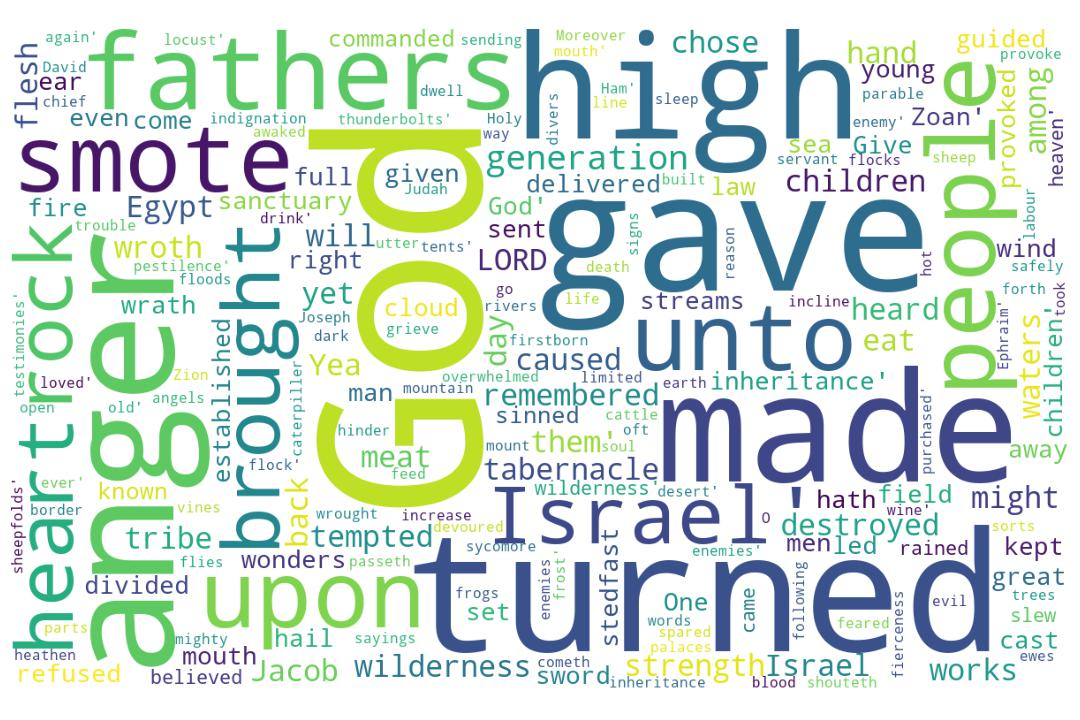
\includegraphics[width=\linewidth]{19OT-Psalms/Psalm78-WordCloud.jpg}
  \caption{Psalm 78 Word Cloud}
  \label{fig:Psalm 78 word Cloud}
\end{figure}

\marginpar{\scriptsize \centering \fcolorbox{bone}{lime}{\textbf{GOD AND HIS PEOPLE}}\\ (Psalm 77) \begin{compactenum}[I.][8]
    \item The  \textbf{Teaching}  \index[scripture]{Psalms!Psa 078:04}(Psa 78:4)
    \item The  \textbf{Testimony}  \index[scripture]{Psalms!Psa 078:05}(Psa 78:5)
    \item The  \textbf{Tempting}  \index[scripture]{Psalms!Psa 078:18}\index[scripture]{Psalms!Psa 078:56} (Psa 78:18, 56)
    \item The  \textbf{Turning}  \index[scripture]{Psalms!Psa 078:41}(Psa 78:41)
    \item The  \textbf{Transgressions}  %\index[scripture]{Psalms!Psa 078:05}(Psalm 78:5)
    \item The  \textbf{Tribe}  \index[scripture]{Psalms!Psa 078:68}(Psa 78:68)
    \item The  \textbf{Tenderness}  \index[scripture]{Psalms!Psa 078:72}(Psa 78:72)
\end{compactenum}}
    




% \textcolor[cmyk]{0.99998,1,0,0}{
\footnote{\textcolor[rgb]{0.00,0.25,0.00}{\hyperlink{TOC}{Return to end of Table of Contents.}}}\footnote{\href{https://audiobible.com/bible/psalms_78.html}{\textcolor[cmyk]{0.99998,1,0,0}{Psalm 78 Audio}}}\textcolor[cmyk]{0.99998,1,0,0}{Maschil of Asaph}\\
\\
\textcolor[cmyk]{0.99998,1,0,0}{Give ear, O my people, \emph{to} my law: incline your ears to the words of my mouth.}
[2] \textcolor[cmyk]{0.99998,1,0,0}{I will open my mouth in a parable: I will utter dark sayings of old:}
[3] \textcolor[cmyk]{0.99998,1,0,0}{Which we have heard and known, and our fathers have told us.}
[4] \textcolor[cmyk]{0.99998,1,0,0}{We will not hide \emph{them} from their children, shewing to the \fcolorbox{bone}{lime}{generation to come} the praises of the LORD, and his strength, and his wonderful works that he hath done.}
[5] \textcolor[cmyk]{0.99998,1,0,0}{For he established a \fcolorbox{bone}{lime}{testimony} in Jacob, and appointed a law in Israel, which he commanded our fathers, that they should make them known to their children:}
[6] \textcolor[cmyk]{0.99998,1,0,0}{That the generation to come might know \emph{them,} \emph{even} the children \emph{which} should be born; \emph{who} should arise and declare \emph{them} to their children:}
[7] \textcolor[cmyk]{0.99998,1,0,0}{That they might set their hope in God, and not forget the works of God, but keep his commandments:}
[8] \textcolor[cmyk]{0.99998,1,0,0}{And might not be as their fathers, a stubborn and rebellious generation; a generation \emph{that} set not their heart aright, and whose spirit was not stedfast with God.}
[9] \textcolor[cmyk]{0.99998,1,0,0}{The children of Ephraim, \emph{being} armed, \emph{and} carrying bows, turned back in the day of battle.}
[10] \textcolor[cmyk]{0.99998,1,0,0}{They kept not the covenant of God, and refused to walk in his law;}
[11] \textcolor[cmyk]{0.99998,1,0,0}{And forgat his works, and his wonders that he had shewed them.}
[12] \textcolor[cmyk]{0.99998,1,0,0}{Marvellous things did he in the sight of their fathers, in the land of Egypt, \emph{in} the field of Zoan.}
[13] \textcolor[cmyk]{0.99998,1,0,0}{He divided the sea, and caused them to pass through; and he made the waters to stand as an heap.}
[14] \textcolor[cmyk]{0.99998,1,0,0}{In the daytime also he led them with a cloud, and all the night with a light of fire.}
[15] \textcolor[cmyk]{0.99998,1,0,0}{He clave the rocks in the wilderness, and gave \emph{them} drink as \emph{out} \emph{of} the great depths.}
[16] \textcolor[cmyk]{0.99998,1,0,0}{He brought streams also out of the rock, and caused waters to run down like rivers.}
[17] \textcolor[cmyk]{0.99998,1,0,0}{And they sinned yet more against him by provoking the most High in the wilderness.}
[18] \textcolor[cmyk]{0.99998,1,0,0}{And they \fcolorbox{bone}{lime}{tempted} God in their heart by asking meat for their lust.}
[19] \textcolor[cmyk]{0.99998,1,0,0}{Yea, they spake against God; they said, Can God furnish a table in the wilderness?}
[20] \textcolor[cmyk]{0.99998,1,0,0}{Behold, he smote the rock, that the waters gushed out, and the streams overflowed; can he give bread also? can he provide flesh for his people?}
[21] \textcolor[cmyk]{0.99998,1,0,0}{Therefore the LORD heard \emph{this}, and was wroth: so a fire was kindled against Jacob, and anger also came up against Israel;}
[22] \textcolor[cmyk]{0.99998,1,0,0}{Because they believed not in God, and trusted not in his salvation:}
[23] \textcolor[cmyk]{0.99998,1,0,0}{Though he had commanded the clouds from above, and opened the doors of heaven,}
[24] \textcolor[cmyk]{0.99998,1,0,0}{And had rained down manna upon them to eat, and had given them of the corn of heaven.}
[25] \textcolor[cmyk]{0.99998,1,0,0}{Man did eat angels' food: he sent them meat to the full.}
[26] \textcolor[cmyk]{0.99998,1,0,0}{He caused an east wind to blow in the heaven: and by his power he brought in the south wind.}
[27] \textcolor[cmyk]{0.99998,1,0,0}{He rained flesh also upon them as dust, and feathered fowls like as the sand of the sea:}
[28] \textcolor[cmyk]{0.99998,1,0,0}{And he let \emph{it} fall in the midst of their camp, round about their habitations.}
[29] \textcolor[cmyk]{0.99998,1,0,0}{So they did eat, and were well filled: for he gave them their own desire;}
[30] \textcolor[cmyk]{0.99998,1,0,0}{They were not estranged from their lust. But while their meat \emph{was} yet in their mouths,}
[31] \textcolor[cmyk]{0.99998,1,0,0}{The wrath of God came upon them, and slew the fattest of them, and smote down the chosen \emph{men} of Israel.}
[32] \textcolor[cmyk]{0.99998,1,0,0}{For all this they sinned still, and believed not for his wondrous works.}
[33] \textcolor[cmyk]{0.99998,1,0,0}{Therefore their days did he consume in vanity, and their years in trouble.}
[34] \textcolor[cmyk]{0.99998,1,0,0}{When he slew them, then they sought him: and they returned and enquired early after God.}
[35] \textcolor[cmyk]{0.99998,1,0,0}{And they remembered that God \emph{was} their rock, and the high God their redeemer.}
[36] \textcolor[cmyk]{0.99998,1,0,0}{Nevertheless they did flatter him with their mouth, and they lied unto him with their tongues.}
[37] \textcolor[cmyk]{0.99998,1,0,0}{For their heart was not right with him, neither were they stedfast in his covenant.}
[38] \textcolor[cmyk]{0.99998,1,0,0}{But he, \emph{being} full of compassion, forgave \emph{their} iniquity, and destroyed \emph{them} not: yea, many a time turned he his anger away, and did not stir up all his wrath.}
[39] \textcolor[cmyk]{0.99998,1,0,0}{For he remembered that they \emph{were} \emph{but} flesh; a wind that passeth away, and cometh not again.}
[40] \textcolor[cmyk]{0.99998,1,0,0}{How oft did they provoke him in the wilderness, \emph{and} grieve him in the desert!}
[41] \textcolor[cmyk]{0.99998,1,0,0}{Yea, they \fcolorbox{bone}{lime}{turned} back and tempted God, and limited the Holy One of Israel.}
[42] \textcolor[cmyk]{0.99998,1,0,0}{They remembered not his hand, \emph{nor} the day when he delivered them from the enemy.}
[43] \textcolor[cmyk]{0.99998,1,0,0}{How he had wrought his signs in Egypt, and his wonders in the field of Zoan:}
[44] \textcolor[cmyk]{0.99998,1,0,0}{And had turned their rivers into blood; and their floods, that they could not drink.}
[45] \textcolor[cmyk]{0.99998,1,0,0}{He sent divers sorts of flies among them, which devoured them; and frogs, which destroyed them.}
[46] \textcolor[cmyk]{0.99998,1,0,0}{He gave also their increase unto the caterpiller, and their labour unto the locust.}
[47] \textcolor[cmyk]{0.99998,1,0,0}{He destroyed their vines with hail, and their sycomore trees with frost.}
[48] \textcolor[cmyk]{0.99998,1,0,0}{He gave up their cattle also to the hail, and their flocks to hot thunderbolts.}
[49] \textcolor[cmyk]{0.99998,1,0,0}{He cast upon them the fierceness of his anger, wrath, and indignation, and trouble, by sending evil angels \emph{among} \emph{them}.}
[50] \textcolor[cmyk]{0.99998,1,0,0}{He made a way to his anger; he spared not their soul from death, but gave their life over to the pestilence;}
[51] \textcolor[cmyk]{0.99998,1,0,0}{And smote all the firstborn in Egypt; the chief of \emph{their} strength in the tabernacles of Ham:}
[52] \textcolor[cmyk]{0.99998,1,0,0}{But made his own people to go forth like sheep, and guided them in the wilderness like a flock.}
[53] \textcolor[cmyk]{0.99998,1,0,0}{And he led them on safely, so that they feared not: but the sea overwhelmed their enemies.}
[54] \textcolor[cmyk]{0.99998,1,0,0}{And he brought them to the border of his sanctuary, \emph{even} \emph{to} this mountain, \emph{which} his right hand had purchased.}
[55] \textcolor[cmyk]{0.99998,1,0,0}{He cast out the heathen also before them, and divided them an inheritance by line, and made the tribes of Israel to dwell in their tents.}
[56] \textcolor[cmyk]{0.99998,1,0,0}{Yet they \fcolorbox{bone}{lime}{tempted} and provoked the most high God, and kept not his testimonies:}
[57] \textcolor[cmyk]{0.99998,1,0,0}{But turned back, and dealt unfaithfully like their fathers: they were turned aside like a deceitful bow.}
[58] \textcolor[cmyk]{0.99998,1,0,0}{For they provoked him to anger with their high places, and moved him to jealousy with their graven images.}
[59] \textcolor[cmyk]{0.99998,1,0,0}{When God heard \emph{this}, he was wroth, and greatly abhorred Israel:}
[60] \textcolor[cmyk]{0.99998,1,0,0}{So that he forsook the tabernacle of Shiloh, the tent \emph{which} he placed among men;}
[61] \textcolor[cmyk]{0.99998,1,0,0}{And delivered his strength into captivity, and his glory into the enemy's hand.}
[62] \textcolor[cmyk]{0.99998,1,0,0}{He gave his people over also unto the sword; and was wroth with his inheritance.}
[63] \textcolor[cmyk]{0.99998,1,0,0}{The fire consumed their young men; and their maidens were not given to marriage.}
[64] \textcolor[cmyk]{0.99998,1,0,0}{Their priests fell by the sword; and their widows made no lamentation.}
[65] \textcolor[cmyk]{0.99998,1,0,0}{Then the Lord awaked as one out of sleep, \emph{and} like a mighty man that shouteth by reason of wine.}
[66] \textcolor[cmyk]{0.99998,1,0,0}{And he smote his enemies in the hinder parts: he put them to a perpetual reproach.}
[67] \textcolor[cmyk]{0.99998,1,0,0}{Moreover he refused the tabernacle of Joseph, and chose not the tribe of Ephraim:}
[68] \textcolor[cmyk]{0.99998,1,0,0}{But chose the \fcolorbox{bone}{lime}{tribe} of Judah, the mount Zion which he loved.}
[69] \textcolor[cmyk]{0.99998,1,0,0}{And he built his sanctuary like high \emph{palaces}, like the earth which he hath established for ever.}
[70] \textcolor[cmyk]{0.99998,1,0,0}{He chose David also his servant, and took him from the sheepfolds:}
[71] \textcolor[cmyk]{0.99998,1,0,0}{From following the ewes great with young he brought him to feed Jacob his people, and Israel his inheritance.}
[72] \textcolor[cmyk]{0.99998,1,0,0}{So he fed them according to the integrity of his heart; and guided them by the \fcolorbox{bone}{lime}{skilfulness} of his hands.}
\section{Psalm 78 Comments}

\subsection{Numeric Nuggets}
Verses 18, 32, 33, and 61 have 13 words.  Verses  2, 19, 23, 32, 41, 45, 48, 51, 56, 60, and 63 have 13 unique words.




%\index[NWIV]{17!Psalms!Psa 78:1}\index[AWIP]{Give!Psalms!Psa 78:1}\index[AWIP]{ear!Psalms!Psa 78:1}\index[AWIP]{O!Psalms!Psa 78:1}\index[AWIP]{my!Psalms!Psa 78:1}\index[AWIP]{my!Psalms!Psa 78:1 (2)}\index[AWIP]{my!Psalms!Psa 78:1 (3)}\index[AWIP]{people!Psalms!Psa 78:1}\index[AWIP]{\emph{to}!Psalms!Psa 78:1}\index[AWIP]{law!Psalms!Psa 78:1}\index[AWIP]{incline!Psalms!Psa 78:1}\index[AWIP]{your!Psalms!Psa 78:1}\index[AWIP]{ears!Psalms!Psa 78:1}\index[AWIP]{to!Psalms!Psa 78:1}\index[AWIP]{the!Psalms!Psa 78:1}\index[AWIP]{words!Psalms!Psa 78:1}\index[AWIP]{of!Psalms!Psa 78:1}\index[AWIP]{mouth!Psalms!Psa 78:1}\index[AWIP]{\emph{to}!Psalms!Psa 78:1}

\index[NWIV]{15!Psalms!Psa 78:2}\index[AWIP]{I!Psalms!Psa 78:2}\index[AWIP]{I!Psalms!Psa 78:2 (2)}\index[AWIP]{will!Psalms!Psa 78:2}\index[AWIP]{will!Psalms!Psa 78:2 (2)}\index[AWIP]{open!Psalms!Psa 78:2}\index[AWIP]{my!Psalms!Psa 78:2}\index[AWIP]{mouth!Psalms!Psa 78:2}\index[AWIP]{in!Psalms!Psa 78:2}\index[AWIP]{a!Psalms!Psa 78:2}\index[AWIP]{parable!Psalms!Psa 78:2}\index[AWIP]{utter!Psalms!Psa 78:2}\index[AWIP]{dark!Psalms!Psa 78:2}\index[AWIP]{sayings!Psalms!Psa 78:2}\index[AWIP]{of!Psalms!Psa 78:2}\index[AWIP]{old!Psalms!Psa 78:2}

\index[NWIV]{12!Psalms!Psa 78:3}\index[AWIP]{Which!Psalms!Psa 78:3}\index[AWIP]{we!Psalms!Psa 78:3}\index[AWIP]{have!Psalms!Psa 78:3}\index[AWIP]{have!Psalms!Psa 78:3 (2)}\index[AWIP]{heard!Psalms!Psa 78:3}\index[AWIP]{and!Psalms!Psa 78:3}\index[AWIP]{and!Psalms!Psa 78:3 (2)}\index[AWIP]{known!Psalms!Psa 78:3}\index[AWIP]{our!Psalms!Psa 78:3}\index[AWIP]{fathers!Psalms!Psa 78:3}\index[AWIP]{told!Psalms!Psa 78:3}\index[AWIP]{us!Psalms!Psa 78:3}

\index[NWIV]{30!Psalms!Psa 78:4}\index[AWIP]{We!Psalms!Psa 78:4}\index[AWIP]{will!Psalms!Psa 78:4}\index[AWIP]{not!Psalms!Psa 78:4}\index[AWIP]{hide!Psalms!Psa 78:4}\index[AWIP]{\emph{them}!Psalms!Psa 78:4}\index[AWIP]{from!Psalms!Psa 78:4}\index[AWIP]{their!Psalms!Psa 78:4}\index[AWIP]{children!Psalms!Psa 78:4}\index[AWIP]{shewing!Psalms!Psa 78:4}\index[AWIP]{to!Psalms!Psa 78:4}\index[AWIP]{to!Psalms!Psa 78:4 (2)}\index[AWIP]{the!Psalms!Psa 78:4}\index[AWIP]{the!Psalms!Psa 78:4 (2)}\index[AWIP]{the!Psalms!Psa 78:4 (3)}\index[AWIP]{generation!Psalms!Psa 78:4}\index[AWIP]{come!Psalms!Psa 78:4}\index[AWIP]{praises!Psalms!Psa 78:4}\index[AWIP]{of!Psalms!Psa 78:4}\index[AWIP]{LORD!Psalms!Psa 78:4}\index[AWIP]{and!Psalms!Psa 78:4}\index[AWIP]{and!Psalms!Psa 78:4 (2)}\index[AWIP]{his!Psalms!Psa 78:4}\index[AWIP]{his!Psalms!Psa 78:4 (2)}\index[AWIP]{strength!Psalms!Psa 78:4}\index[AWIP]{wonderful!Psalms!Psa 78:4}\index[AWIP]{works!Psalms!Psa 78:4}\index[AWIP]{that!Psalms!Psa 78:4}\index[AWIP]{he!Psalms!Psa 78:4}\index[AWIP]{hath!Psalms!Psa 78:4}\index[AWIP]{done!Psalms!Psa 78:4}\index[AWIP]{\emph{them}!Psalms!Psa 78:4}

\index[NWIV]{27!Psalms!Psa 78:5}\index[AWIP]{For!Psalms!Psa 78:5}\index[AWIP]{he!Psalms!Psa 78:5}\index[AWIP]{he!Psalms!Psa 78:5 (2)}\index[AWIP]{established!Psalms!Psa 78:5}\index[AWIP]{a!Psalms!Psa 78:5}\index[AWIP]{a!Psalms!Psa 78:5 (2)}\index[AWIP]{testimony!Psalms!Psa 78:5}\index[AWIP]{in!Psalms!Psa 78:5}\index[AWIP]{in!Psalms!Psa 78:5 (2)}\index[AWIP]{Jacob!Psalms!Psa 78:5}\index[AWIP]{and!Psalms!Psa 78:5}\index[AWIP]{appointed!Psalms!Psa 78:5}\index[AWIP]{law!Psalms!Psa 78:5}\index[AWIP]{Israel!Psalms!Psa 78:5}\index[AWIP]{which!Psalms!Psa 78:5}\index[AWIP]{commanded!Psalms!Psa 78:5}\index[AWIP]{our!Psalms!Psa 78:5}\index[AWIP]{fathers!Psalms!Psa 78:5}\index[AWIP]{that!Psalms!Psa 78:5}\index[AWIP]{they!Psalms!Psa 78:5}\index[AWIP]{should!Psalms!Psa 78:5}\index[AWIP]{make!Psalms!Psa 78:5}\index[AWIP]{them!Psalms!Psa 78:5}\index[AWIP]{known!Psalms!Psa 78:5}\index[AWIP]{to!Psalms!Psa 78:5}\index[AWIP]{their!Psalms!Psa 78:5}\index[AWIP]{children!Psalms!Psa 78:5}

\index[NWIV]{24!Psalms!Psa 78:6}\index[AWIP]{That!Psalms!Psa 78:6}\index[AWIP]{the!Psalms!Psa 78:6}\index[AWIP]{the!Psalms!Psa 78:6 (2)}\index[AWIP]{generation!Psalms!Psa 78:6}\index[AWIP]{to!Psalms!Psa 78:6}\index[AWIP]{to!Psalms!Psa 78:6 (2)}\index[AWIP]{come!Psalms!Psa 78:6}\index[AWIP]{might!Psalms!Psa 78:6}\index[AWIP]{know!Psalms!Psa 78:6}\index[AWIP]{\emph{them}!Psalms!Psa 78:6}\index[AWIP]{\emph{them}!Psalms!Psa 78:6 (2)}\index[AWIP]{\emph{even}!Psalms!Psa 78:6}\index[AWIP]{children!Psalms!Psa 78:6}\index[AWIP]{children!Psalms!Psa 78:6 (2)}\index[AWIP]{\emph{which}!Psalms!Psa 78:6}\index[AWIP]{should!Psalms!Psa 78:6}\index[AWIP]{should!Psalms!Psa 78:6 (2)}\index[AWIP]{be!Psalms!Psa 78:6}\index[AWIP]{born!Psalms!Psa 78:6}\index[AWIP]{\emph{who}!Psalms!Psa 78:6}\index[AWIP]{arise!Psalms!Psa 78:6}\index[AWIP]{and!Psalms!Psa 78:6}\index[AWIP]{declare!Psalms!Psa 78:6}\index[AWIP]{their!Psalms!Psa 78:6}\index[AWIP]{\emph{them}!Psalms!Psa 78:6}\index[AWIP]{\emph{them}!Psalms!Psa 78:6 (2)}\index[AWIP]{\emph{even}!Psalms!Psa 78:6}\index[AWIP]{\emph{which}!Psalms!Psa 78:6}\index[AWIP]{\emph{who}!Psalms!Psa 78:6}

\index[NWIV]{19!Psalms!Psa 78:7}\index[AWIP]{That!Psalms!Psa 78:7}\index[AWIP]{they!Psalms!Psa 78:7}\index[AWIP]{might!Psalms!Psa 78:7}\index[AWIP]{set!Psalms!Psa 78:7}\index[AWIP]{their!Psalms!Psa 78:7}\index[AWIP]{hope!Psalms!Psa 78:7}\index[AWIP]{in!Psalms!Psa 78:7}\index[AWIP]{God!Psalms!Psa 78:7}\index[AWIP]{God!Psalms!Psa 78:7 (2)}\index[AWIP]{and!Psalms!Psa 78:7}\index[AWIP]{not!Psalms!Psa 78:7}\index[AWIP]{forget!Psalms!Psa 78:7}\index[AWIP]{the!Psalms!Psa 78:7}\index[AWIP]{works!Psalms!Psa 78:7}\index[AWIP]{of!Psalms!Psa 78:7}\index[AWIP]{but!Psalms!Psa 78:7}\index[AWIP]{keep!Psalms!Psa 78:7}\index[AWIP]{his!Psalms!Psa 78:7}\index[AWIP]{commandments!Psalms!Psa 78:7}

\index[NWIV]{28!Psalms!Psa 78:8}\index[AWIP]{And!Psalms!Psa 78:8}\index[AWIP]{might!Psalms!Psa 78:8}\index[AWIP]{not!Psalms!Psa 78:8}\index[AWIP]{not!Psalms!Psa 78:8 (2)}\index[AWIP]{not!Psalms!Psa 78:8 (3)}\index[AWIP]{be!Psalms!Psa 78:8}\index[AWIP]{as!Psalms!Psa 78:8}\index[AWIP]{their!Psalms!Psa 78:8}\index[AWIP]{their!Psalms!Psa 78:8 (2)}\index[AWIP]{fathers!Psalms!Psa 78:8}\index[AWIP]{a!Psalms!Psa 78:8}\index[AWIP]{a!Psalms!Psa 78:8 (2)}\index[AWIP]{stubborn!Psalms!Psa 78:8}\index[AWIP]{and!Psalms!Psa 78:8}\index[AWIP]{and!Psalms!Psa 78:8 (2)}\index[AWIP]{rebellious!Psalms!Psa 78:8}\index[AWIP]{generation!Psalms!Psa 78:8}\index[AWIP]{generation!Psalms!Psa 78:8 (2)}\index[AWIP]{\emph{that}!Psalms!Psa 78:8}\index[AWIP]{set!Psalms!Psa 78:8}\index[AWIP]{heart!Psalms!Psa 78:8}\index[AWIP]{aright!Psalms!Psa 78:8}\index[AWIP]{whose!Psalms!Psa 78:8}\index[AWIP]{spirit!Psalms!Psa 78:8}\index[AWIP]{was!Psalms!Psa 78:8}\index[AWIP]{stedfast!Psalms!Psa 78:8}\index[AWIP]{with!Psalms!Psa 78:8}\index[AWIP]{God!Psalms!Psa 78:8}\index[AWIP]{\emph{that}!Psalms!Psa 78:8}

\index[NWIV]{16!Psalms!Psa 78:9}\index[AWIP]{The!Psalms!Psa 78:9}\index[AWIP]{children!Psalms!Psa 78:9}\index[AWIP]{of!Psalms!Psa 78:9}\index[AWIP]{of!Psalms!Psa 78:9 (2)}\index[AWIP]{Ephraim!Psalms!Psa 78:9}\index[AWIP]{\emph{being}!Psalms!Psa 78:9}\index[AWIP]{armed!Psalms!Psa 78:9}\index[AWIP]{\emph{and}!Psalms!Psa 78:9}\index[AWIP]{carrying!Psalms!Psa 78:9}\index[AWIP]{bows!Psalms!Psa 78:9}\index[AWIP]{turned!Psalms!Psa 78:9}\index[AWIP]{back!Psalms!Psa 78:9}\index[AWIP]{in!Psalms!Psa 78:9}\index[AWIP]{the!Psalms!Psa 78:9}\index[AWIP]{day!Psalms!Psa 78:9}\index[AWIP]{battle!Psalms!Psa 78:9}\index[AWIP]{\emph{being}!Psalms!Psa 78:9}\index[AWIP]{\emph{and}!Psalms!Psa 78:9}

\index[NWIV]{14!Psalms!Psa 78:10}\index[AWIP]{They!Psalms!Psa 78:10}\index[AWIP]{kept!Psalms!Psa 78:10}\index[AWIP]{not!Psalms!Psa 78:10}\index[AWIP]{the!Psalms!Psa 78:10}\index[AWIP]{covenant!Psalms!Psa 78:10}\index[AWIP]{of!Psalms!Psa 78:10}\index[AWIP]{God!Psalms!Psa 78:10}\index[AWIP]{and!Psalms!Psa 78:10}\index[AWIP]{refused!Psalms!Psa 78:10}\index[AWIP]{to!Psalms!Psa 78:10}\index[AWIP]{walk!Psalms!Psa 78:10}\index[AWIP]{in!Psalms!Psa 78:10}\index[AWIP]{his!Psalms!Psa 78:10}\index[AWIP]{law!Psalms!Psa 78:10}

\index[NWIV]{12!Psalms!Psa 78:11}\index[AWIP]{And!Psalms!Psa 78:11}\index[AWIP]{forgat!Psalms!Psa 78:11}\index[AWIP]{his!Psalms!Psa 78:11}\index[AWIP]{his!Psalms!Psa 78:11 (2)}\index[AWIP]{works!Psalms!Psa 78:11}\index[AWIP]{and!Psalms!Psa 78:11}\index[AWIP]{wonders!Psalms!Psa 78:11}\index[AWIP]{that!Psalms!Psa 78:11}\index[AWIP]{he!Psalms!Psa 78:11}\index[AWIP]{had!Psalms!Psa 78:11}\index[AWIP]{shewed!Psalms!Psa 78:11}\index[AWIP]{them!Psalms!Psa 78:11}

\index[NWIV]{20!Psalms!Psa 78:12}\index[AWIP]{Marvellous!Psalms!Psa 78:12}\index[AWIP]{things!Psalms!Psa 78:12}\index[AWIP]{did!Psalms!Psa 78:12}\index[AWIP]{he!Psalms!Psa 78:12}\index[AWIP]{in!Psalms!Psa 78:12}\index[AWIP]{in!Psalms!Psa 78:12 (2)}\index[AWIP]{the!Psalms!Psa 78:12}\index[AWIP]{the!Psalms!Psa 78:12 (2)}\index[AWIP]{the!Psalms!Psa 78:12 (3)}\index[AWIP]{sight!Psalms!Psa 78:12}\index[AWIP]{of!Psalms!Psa 78:12}\index[AWIP]{of!Psalms!Psa 78:12 (2)}\index[AWIP]{of!Psalms!Psa 78:12 (3)}\index[AWIP]{their!Psalms!Psa 78:12}\index[AWIP]{fathers!Psalms!Psa 78:12}\index[AWIP]{land!Psalms!Psa 78:12}\index[AWIP]{Egypt!Psalms!Psa 78:12}\index[AWIP]{\emph{in}!Psalms!Psa 78:12}\index[AWIP]{field!Psalms!Psa 78:12}\index[AWIP]{Zoan!Psalms!Psa 78:12}\index[AWIP]{\emph{in}!Psalms!Psa 78:12}

\index[NWIV]{20!Psalms!Psa 78:13}\index[AWIP]{He!Psalms!Psa 78:13}\index[AWIP]{divided!Psalms!Psa 78:13}\index[AWIP]{the!Psalms!Psa 78:13}\index[AWIP]{the!Psalms!Psa 78:13 (2)}\index[AWIP]{sea!Psalms!Psa 78:13}\index[AWIP]{and!Psalms!Psa 78:13}\index[AWIP]{and!Psalms!Psa 78:13 (2)}\index[AWIP]{caused!Psalms!Psa 78:13}\index[AWIP]{them!Psalms!Psa 78:13}\index[AWIP]{to!Psalms!Psa 78:13}\index[AWIP]{to!Psalms!Psa 78:13 (2)}\index[AWIP]{pass!Psalms!Psa 78:13}\index[AWIP]{through!Psalms!Psa 78:13}\index[AWIP]{he!Psalms!Psa 78:13}\index[AWIP]{made!Psalms!Psa 78:13}\index[AWIP]{waters!Psalms!Psa 78:13}\index[AWIP]{stand!Psalms!Psa 78:13}\index[AWIP]{as!Psalms!Psa 78:13}\index[AWIP]{an!Psalms!Psa 78:13}\index[AWIP]{heap!Psalms!Psa 78:13}

\index[NWIV]{19!Psalms!Psa 78:14}\index[AWIP]{In!Psalms!Psa 78:14}\index[AWIP]{the!Psalms!Psa 78:14}\index[AWIP]{the!Psalms!Psa 78:14 (2)}\index[AWIP]{daytime!Psalms!Psa 78:14}\index[AWIP]{also!Psalms!Psa 78:14}\index[AWIP]{he!Psalms!Psa 78:14}\index[AWIP]{led!Psalms!Psa 78:14}\index[AWIP]{them!Psalms!Psa 78:14}\index[AWIP]{with!Psalms!Psa 78:14}\index[AWIP]{with!Psalms!Psa 78:14 (2)}\index[AWIP]{a!Psalms!Psa 78:14}\index[AWIP]{a!Psalms!Psa 78:14 (2)}\index[AWIP]{cloud!Psalms!Psa 78:14}\index[AWIP]{and!Psalms!Psa 78:14}\index[AWIP]{all!Psalms!Psa 78:14}\index[AWIP]{night!Psalms!Psa 78:14}\index[AWIP]{light!Psalms!Psa 78:14}\index[AWIP]{of!Psalms!Psa 78:14}\index[AWIP]{fire!Psalms!Psa 78:14}

\index[NWIV]{17!Psalms!Psa 78:15}\index[AWIP]{He!Psalms!Psa 78:15}\index[AWIP]{clave!Psalms!Psa 78:15}\index[AWIP]{the!Psalms!Psa 78:15}\index[AWIP]{the!Psalms!Psa 78:15 (2)}\index[AWIP]{the!Psalms!Psa 78:15 (3)}\index[AWIP]{rocks!Psalms!Psa 78:15}\index[AWIP]{in!Psalms!Psa 78:15}\index[AWIP]{wilderness!Psalms!Psa 78:15}\index[AWIP]{and!Psalms!Psa 78:15}\index[AWIP]{gave!Psalms!Psa 78:15}\index[AWIP]{\emph{them}!Psalms!Psa 78:15}\index[AWIP]{drink!Psalms!Psa 78:15}\index[AWIP]{as!Psalms!Psa 78:15}\index[AWIP]{\emph{out}!Psalms!Psa 78:15}\index[AWIP]{\emph{of}!Psalms!Psa 78:15}\index[AWIP]{great!Psalms!Psa 78:15}\index[AWIP]{depths!Psalms!Psa 78:15}\index[AWIP]{\emph{them}!Psalms!Psa 78:15}\index[AWIP]{\emph{out}!Psalms!Psa 78:15}\index[AWIP]{\emph{of}!Psalms!Psa 78:15}

\index[NWIV]{16!Psalms!Psa 78:16}\index[AWIP]{He!Psalms!Psa 78:16}\index[AWIP]{brought!Psalms!Psa 78:16}\index[AWIP]{streams!Psalms!Psa 78:16}\index[AWIP]{also!Psalms!Psa 78:16}\index[AWIP]{out!Psalms!Psa 78:16}\index[AWIP]{of!Psalms!Psa 78:16}\index[AWIP]{the!Psalms!Psa 78:16}\index[AWIP]{rock!Psalms!Psa 78:16}\index[AWIP]{and!Psalms!Psa 78:16}\index[AWIP]{caused!Psalms!Psa 78:16}\index[AWIP]{waters!Psalms!Psa 78:16}\index[AWIP]{to!Psalms!Psa 78:16}\index[AWIP]{run!Psalms!Psa 78:16}\index[AWIP]{down!Psalms!Psa 78:16}\index[AWIP]{like!Psalms!Psa 78:16}\index[AWIP]{rivers!Psalms!Psa 78:16}

\index[NWIV]{15!Psalms!Psa 78:17}\index[AWIP]{And!Psalms!Psa 78:17}\index[AWIP]{they!Psalms!Psa 78:17}\index[AWIP]{sinned!Psalms!Psa 78:17}\index[AWIP]{yet!Psalms!Psa 78:17}\index[AWIP]{more!Psalms!Psa 78:17}\index[AWIP]{against!Psalms!Psa 78:17}\index[AWIP]{him!Psalms!Psa 78:17}\index[AWIP]{by!Psalms!Psa 78:17}\index[AWIP]{provoking!Psalms!Psa 78:17}\index[AWIP]{the!Psalms!Psa 78:17}\index[AWIP]{the!Psalms!Psa 78:17 (2)}\index[AWIP]{most!Psalms!Psa 78:17}\index[AWIP]{High!Psalms!Psa 78:17}\index[AWIP]{in!Psalms!Psa 78:17}\index[AWIP]{wilderness!Psalms!Psa 78:17}

\index[NWIV]{13!Psalms!Psa 78:18}\index[AWIP]{And!Psalms!Psa 78:18}\index[AWIP]{they!Psalms!Psa 78:18}\index[AWIP]{tempted!Psalms!Psa 78:18}\index[AWIP]{God!Psalms!Psa 78:18}\index[AWIP]{in!Psalms!Psa 78:18}\index[AWIP]{their!Psalms!Psa 78:18}\index[AWIP]{their!Psalms!Psa 78:18 (2)}\index[AWIP]{heart!Psalms!Psa 78:18}\index[AWIP]{by!Psalms!Psa 78:18}\index[AWIP]{asking!Psalms!Psa 78:18}\index[AWIP]{meat!Psalms!Psa 78:18}\index[AWIP]{for!Psalms!Psa 78:18}\index[AWIP]{lust!Psalms!Psa 78:18}

\index[NWIV]{15!Psalms!Psa 78:19}\index[AWIP]{Yea!Psalms!Psa 78:19}\index[AWIP]{they!Psalms!Psa 78:19}\index[AWIP]{they!Psalms!Psa 78:19 (2)}\index[AWIP]{spake!Psalms!Psa 78:19}\index[AWIP]{against!Psalms!Psa 78:19}\index[AWIP]{God!Psalms!Psa 78:19}\index[AWIP]{God!Psalms!Psa 78:19 (2)}\index[AWIP]{said!Psalms!Psa 78:19}\index[AWIP]{Can!Psalms!Psa 78:19}\index[AWIP]{furnish!Psalms!Psa 78:19}\index[AWIP]{a!Psalms!Psa 78:19}\index[AWIP]{table!Psalms!Psa 78:19}\index[AWIP]{in!Psalms!Psa 78:19}\index[AWIP]{the!Psalms!Psa 78:19}\index[AWIP]{wilderness?!Psalms!Psa 78:19}

\index[NWIV]{26!Psalms!Psa 78:20}\index[AWIP]{Behold!Psalms!Psa 78:20}\index[AWIP]{he!Psalms!Psa 78:20}\index[AWIP]{he!Psalms!Psa 78:20 (2)}\index[AWIP]{he!Psalms!Psa 78:20 (3)}\index[AWIP]{smote!Psalms!Psa 78:20}\index[AWIP]{the!Psalms!Psa 78:20}\index[AWIP]{the!Psalms!Psa 78:20 (2)}\index[AWIP]{the!Psalms!Psa 78:20 (3)}\index[AWIP]{rock!Psalms!Psa 78:20}\index[AWIP]{that!Psalms!Psa 78:20}\index[AWIP]{waters!Psalms!Psa 78:20}\index[AWIP]{gushed!Psalms!Psa 78:20}\index[AWIP]{out!Psalms!Psa 78:20}\index[AWIP]{and!Psalms!Psa 78:20}\index[AWIP]{streams!Psalms!Psa 78:20}\index[AWIP]{overflowed!Psalms!Psa 78:20}\index[AWIP]{can!Psalms!Psa 78:20}\index[AWIP]{can!Psalms!Psa 78:20 (2)}\index[AWIP]{give!Psalms!Psa 78:20}\index[AWIP]{bread!Psalms!Psa 78:20}\index[AWIP]{also?!Psalms!Psa 78:20}\index[AWIP]{provide!Psalms!Psa 78:20}\index[AWIP]{flesh!Psalms!Psa 78:20}\index[AWIP]{for!Psalms!Psa 78:20}\index[AWIP]{his!Psalms!Psa 78:20}\index[AWIP]{people?!Psalms!Psa 78:20}

\index[NWIV]{22!Psalms!Psa 78:21}\index[AWIP]{Therefore!Psalms!Psa 78:21}\index[AWIP]{the!Psalms!Psa 78:21}\index[AWIP]{LORD!Psalms!Psa 78:21}\index[AWIP]{heard!Psalms!Psa 78:21}\index[AWIP]{\emph{this}!Psalms!Psa 78:21}\index[AWIP]{and!Psalms!Psa 78:21}\index[AWIP]{and!Psalms!Psa 78:21 (2)}\index[AWIP]{was!Psalms!Psa 78:21}\index[AWIP]{was!Psalms!Psa 78:21 (2)}\index[AWIP]{wroth!Psalms!Psa 78:21}\index[AWIP]{so!Psalms!Psa 78:21}\index[AWIP]{a!Psalms!Psa 78:21}\index[AWIP]{fire!Psalms!Psa 78:21}\index[AWIP]{kindled!Psalms!Psa 78:21}\index[AWIP]{against!Psalms!Psa 78:21}\index[AWIP]{against!Psalms!Psa 78:21 (2)}\index[AWIP]{Jacob!Psalms!Psa 78:21}\index[AWIP]{anger!Psalms!Psa 78:21}\index[AWIP]{also!Psalms!Psa 78:21}\index[AWIP]{came!Psalms!Psa 78:21}\index[AWIP]{up!Psalms!Psa 78:21}\index[AWIP]{Israel!Psalms!Psa 78:21}\index[AWIP]{\emph{this}!Psalms!Psa 78:21}

\index[NWIV]{12!Psalms!Psa 78:22}\index[AWIP]{Because!Psalms!Psa 78:22}\index[AWIP]{they!Psalms!Psa 78:22}\index[AWIP]{believed!Psalms!Psa 78:22}\index[AWIP]{not!Psalms!Psa 78:22}\index[AWIP]{not!Psalms!Psa 78:22 (2)}\index[AWIP]{in!Psalms!Psa 78:22}\index[AWIP]{in!Psalms!Psa 78:22 (2)}\index[AWIP]{God!Psalms!Psa 78:22}\index[AWIP]{and!Psalms!Psa 78:22}\index[AWIP]{trusted!Psalms!Psa 78:22}\index[AWIP]{his!Psalms!Psa 78:22}\index[AWIP]{salvation!Psalms!Psa 78:22}

\index[NWIV]{14!Psalms!Psa 78:23}\index[AWIP]{Though!Psalms!Psa 78:23}\index[AWIP]{he!Psalms!Psa 78:23}\index[AWIP]{had!Psalms!Psa 78:23}\index[AWIP]{commanded!Psalms!Psa 78:23}\index[AWIP]{the!Psalms!Psa 78:23}\index[AWIP]{the!Psalms!Psa 78:23 (2)}\index[AWIP]{clouds!Psalms!Psa 78:23}\index[AWIP]{from!Psalms!Psa 78:23}\index[AWIP]{above!Psalms!Psa 78:23}\index[AWIP]{and!Psalms!Psa 78:23}\index[AWIP]{opened!Psalms!Psa 78:23}\index[AWIP]{doors!Psalms!Psa 78:23}\index[AWIP]{of!Psalms!Psa 78:23}\index[AWIP]{heaven!Psalms!Psa 78:23}

\index[NWIV]{18!Psalms!Psa 78:24}\index[AWIP]{And!Psalms!Psa 78:24}\index[AWIP]{had!Psalms!Psa 78:24}\index[AWIP]{had!Psalms!Psa 78:24 (2)}\index[AWIP]{rained!Psalms!Psa 78:24}\index[AWIP]{down!Psalms!Psa 78:24}\index[AWIP]{manna!Psalms!Psa 78:24}\index[AWIP]{upon!Psalms!Psa 78:24}\index[AWIP]{them!Psalms!Psa 78:24}\index[AWIP]{them!Psalms!Psa 78:24 (2)}\index[AWIP]{to!Psalms!Psa 78:24}\index[AWIP]{eat!Psalms!Psa 78:24}\index[AWIP]{and!Psalms!Psa 78:24}\index[AWIP]{given!Psalms!Psa 78:24}\index[AWIP]{of!Psalms!Psa 78:24}\index[AWIP]{of!Psalms!Psa 78:24 (2)}\index[AWIP]{the!Psalms!Psa 78:24}\index[AWIP]{corn!Psalms!Psa 78:24}\index[AWIP]{heaven!Psalms!Psa 78:24}

\index[NWIV]{12!Psalms!Psa 78:25}\index[AWIP]{Man!Psalms!Psa 78:25}\index[AWIP]{did!Psalms!Psa 78:25}\index[AWIP]{eat!Psalms!Psa 78:25}\index[AWIP]{angels'!Psalms!Psa 78:25}\index[AWIP]{food!Psalms!Psa 78:25}\index[AWIP]{he!Psalms!Psa 78:25}\index[AWIP]{sent!Psalms!Psa 78:25}\index[AWIP]{them!Psalms!Psa 78:25}\index[AWIP]{meat!Psalms!Psa 78:25}\index[AWIP]{to!Psalms!Psa 78:25}\index[AWIP]{the!Psalms!Psa 78:25}\index[AWIP]{full!Psalms!Psa 78:25}

\index[NWIV]{20!Psalms!Psa 78:26}\index[AWIP]{He!Psalms!Psa 78:26}\index[AWIP]{caused!Psalms!Psa 78:26}\index[AWIP]{an!Psalms!Psa 78:26}\index[AWIP]{east!Psalms!Psa 78:26}\index[AWIP]{wind!Psalms!Psa 78:26}\index[AWIP]{wind!Psalms!Psa 78:26 (2)}\index[AWIP]{to!Psalms!Psa 78:26}\index[AWIP]{blow!Psalms!Psa 78:26}\index[AWIP]{in!Psalms!Psa 78:26}\index[AWIP]{in!Psalms!Psa 78:26 (2)}\index[AWIP]{the!Psalms!Psa 78:26}\index[AWIP]{the!Psalms!Psa 78:26 (2)}\index[AWIP]{heaven!Psalms!Psa 78:26}\index[AWIP]{and!Psalms!Psa 78:26}\index[AWIP]{by!Psalms!Psa 78:26}\index[AWIP]{his!Psalms!Psa 78:26}\index[AWIP]{power!Psalms!Psa 78:26}\index[AWIP]{he!Psalms!Psa 78:26}\index[AWIP]{brought!Psalms!Psa 78:26}\index[AWIP]{south!Psalms!Psa 78:26}

\index[NWIV]{18!Psalms!Psa 78:27}\index[AWIP]{He!Psalms!Psa 78:27}\index[AWIP]{rained!Psalms!Psa 78:27}\index[AWIP]{flesh!Psalms!Psa 78:27}\index[AWIP]{also!Psalms!Psa 78:27}\index[AWIP]{upon!Psalms!Psa 78:27}\index[AWIP]{them!Psalms!Psa 78:27}\index[AWIP]{as!Psalms!Psa 78:27}\index[AWIP]{as!Psalms!Psa 78:27 (2)}\index[AWIP]{dust!Psalms!Psa 78:27}\index[AWIP]{and!Psalms!Psa 78:27}\index[AWIP]{feathered!Psalms!Psa 78:27}\index[AWIP]{fowls!Psalms!Psa 78:27}\index[AWIP]{like!Psalms!Psa 78:27}\index[AWIP]{the!Psalms!Psa 78:27}\index[AWIP]{the!Psalms!Psa 78:27 (2)}\index[AWIP]{sand!Psalms!Psa 78:27}\index[AWIP]{of!Psalms!Psa 78:27}\index[AWIP]{sea!Psalms!Psa 78:27}

\index[NWIV]{15!Psalms!Psa 78:28}\index[AWIP]{And!Psalms!Psa 78:28}\index[AWIP]{he!Psalms!Psa 78:28}\index[AWIP]{let!Psalms!Psa 78:28}\index[AWIP]{\emph{it}!Psalms!Psa 78:28}\index[AWIP]{fall!Psalms!Psa 78:28}\index[AWIP]{in!Psalms!Psa 78:28}\index[AWIP]{the!Psalms!Psa 78:28}\index[AWIP]{midst!Psalms!Psa 78:28}\index[AWIP]{of!Psalms!Psa 78:28}\index[AWIP]{their!Psalms!Psa 78:28}\index[AWIP]{their!Psalms!Psa 78:28 (2)}\index[AWIP]{camp!Psalms!Psa 78:28}\index[AWIP]{round!Psalms!Psa 78:28}\index[AWIP]{about!Psalms!Psa 78:28}\index[AWIP]{habitations!Psalms!Psa 78:28}\index[AWIP]{\emph{it}!Psalms!Psa 78:28}

\index[NWIV]{15!Psalms!Psa 78:29}\index[AWIP]{So!Psalms!Psa 78:29}\index[AWIP]{they!Psalms!Psa 78:29}\index[AWIP]{did!Psalms!Psa 78:29}\index[AWIP]{eat!Psalms!Psa 78:29}\index[AWIP]{and!Psalms!Psa 78:29}\index[AWIP]{were!Psalms!Psa 78:29}\index[AWIP]{well!Psalms!Psa 78:29}\index[AWIP]{filled!Psalms!Psa 78:29}\index[AWIP]{for!Psalms!Psa 78:29}\index[AWIP]{he!Psalms!Psa 78:29}\index[AWIP]{gave!Psalms!Psa 78:29}\index[AWIP]{them!Psalms!Psa 78:29}\index[AWIP]{their!Psalms!Psa 78:29}\index[AWIP]{own!Psalms!Psa 78:29}\index[AWIP]{desire!Psalms!Psa 78:29}

\index[NWIV]{16!Psalms!Psa 78:30}\index[AWIP]{They!Psalms!Psa 78:30}\index[AWIP]{were!Psalms!Psa 78:30}\index[AWIP]{not!Psalms!Psa 78:30}\index[AWIP]{estranged!Psalms!Psa 78:30}\index[AWIP]{from!Psalms!Psa 78:30}\index[AWIP]{their!Psalms!Psa 78:30}\index[AWIP]{their!Psalms!Psa 78:30 (2)}\index[AWIP]{their!Psalms!Psa 78:30 (3)}\index[AWIP]{lust!Psalms!Psa 78:30}\index[AWIP]{But!Psalms!Psa 78:30}\index[AWIP]{while!Psalms!Psa 78:30}\index[AWIP]{meat!Psalms!Psa 78:30}\index[AWIP]{\emph{was}!Psalms!Psa 78:30}\index[AWIP]{yet!Psalms!Psa 78:30}\index[AWIP]{in!Psalms!Psa 78:30}\index[AWIP]{mouths!Psalms!Psa 78:30}\index[AWIP]{\emph{was}!Psalms!Psa 78:30}

\index[NWIV]{21!Psalms!Psa 78:31}\index[AWIP]{The!Psalms!Psa 78:31}\index[AWIP]{wrath!Psalms!Psa 78:31}\index[AWIP]{of!Psalms!Psa 78:31}\index[AWIP]{of!Psalms!Psa 78:31 (2)}\index[AWIP]{of!Psalms!Psa 78:31 (3)}\index[AWIP]{God!Psalms!Psa 78:31}\index[AWIP]{came!Psalms!Psa 78:31}\index[AWIP]{upon!Psalms!Psa 78:31}\index[AWIP]{them!Psalms!Psa 78:31}\index[AWIP]{them!Psalms!Psa 78:31 (2)}\index[AWIP]{and!Psalms!Psa 78:31}\index[AWIP]{and!Psalms!Psa 78:31 (2)}\index[AWIP]{slew!Psalms!Psa 78:31}\index[AWIP]{the!Psalms!Psa 78:31}\index[AWIP]{the!Psalms!Psa 78:31 (2)}\index[AWIP]{fattest!Psalms!Psa 78:31}\index[AWIP]{smote!Psalms!Psa 78:31}\index[AWIP]{down!Psalms!Psa 78:31}\index[AWIP]{chosen!Psalms!Psa 78:31}\index[AWIP]{\emph{men}!Psalms!Psa 78:31}\index[AWIP]{Israel!Psalms!Psa 78:31}\index[AWIP]{\emph{men}!Psalms!Psa 78:31}

\index[NWIV]{13!Psalms!Psa 78:32}\index[AWIP]{For!Psalms!Psa 78:32}\index[AWIP]{all!Psalms!Psa 78:32}\index[AWIP]{this!Psalms!Psa 78:32}\index[AWIP]{they!Psalms!Psa 78:32}\index[AWIP]{sinned!Psalms!Psa 78:32}\index[AWIP]{still!Psalms!Psa 78:32}\index[AWIP]{and!Psalms!Psa 78:32}\index[AWIP]{believed!Psalms!Psa 78:32}\index[AWIP]{not!Psalms!Psa 78:32}\index[AWIP]{for!Psalms!Psa 78:32}\index[AWIP]{his!Psalms!Psa 78:32}\index[AWIP]{wondrous!Psalms!Psa 78:32}\index[AWIP]{works!Psalms!Psa 78:32}

\index[NWIV]{13!Psalms!Psa 78:33}\index[AWIP]{Therefore!Psalms!Psa 78:33}\index[AWIP]{their!Psalms!Psa 78:33}\index[AWIP]{their!Psalms!Psa 78:33 (2)}\index[AWIP]{days!Psalms!Psa 78:33}\index[AWIP]{did!Psalms!Psa 78:33}\index[AWIP]{he!Psalms!Psa 78:33}\index[AWIP]{consume!Psalms!Psa 78:33}\index[AWIP]{in!Psalms!Psa 78:33}\index[AWIP]{in!Psalms!Psa 78:33 (2)}\index[AWIP]{vanity!Psalms!Psa 78:33}\index[AWIP]{and!Psalms!Psa 78:33}\index[AWIP]{years!Psalms!Psa 78:33}\index[AWIP]{trouble!Psalms!Psa 78:33}

\index[NWIV]{16!Psalms!Psa 78:34}\index[AWIP]{When!Psalms!Psa 78:34}\index[AWIP]{he!Psalms!Psa 78:34}\index[AWIP]{slew!Psalms!Psa 78:34}\index[AWIP]{them!Psalms!Psa 78:34}\index[AWIP]{then!Psalms!Psa 78:34}\index[AWIP]{they!Psalms!Psa 78:34}\index[AWIP]{they!Psalms!Psa 78:34 (2)}\index[AWIP]{sought!Psalms!Psa 78:34}\index[AWIP]{him!Psalms!Psa 78:34}\index[AWIP]{and!Psalms!Psa 78:34}\index[AWIP]{and!Psalms!Psa 78:34 (2)}\index[AWIP]{returned!Psalms!Psa 78:34}\index[AWIP]{enquired!Psalms!Psa 78:34}\index[AWIP]{early!Psalms!Psa 78:34}\index[AWIP]{after!Psalms!Psa 78:34}\index[AWIP]{God!Psalms!Psa 78:34}

\index[NWIV]{14!Psalms!Psa 78:35}\index[AWIP]{And!Psalms!Psa 78:35}\index[AWIP]{they!Psalms!Psa 78:35}\index[AWIP]{remembered!Psalms!Psa 78:35}\index[AWIP]{that!Psalms!Psa 78:35}\index[AWIP]{God!Psalms!Psa 78:35}\index[AWIP]{God!Psalms!Psa 78:35 (2)}\index[AWIP]{\emph{was}!Psalms!Psa 78:35}\index[AWIP]{their!Psalms!Psa 78:35}\index[AWIP]{their!Psalms!Psa 78:35 (2)}\index[AWIP]{rock!Psalms!Psa 78:35}\index[AWIP]{and!Psalms!Psa 78:35}\index[AWIP]{the!Psalms!Psa 78:35}\index[AWIP]{high!Psalms!Psa 78:35}\index[AWIP]{redeemer!Psalms!Psa 78:35}\index[AWIP]{\emph{was}!Psalms!Psa 78:35}

\index[NWIV]{16!Psalms!Psa 78:36}\index[AWIP]{Nevertheless!Psalms!Psa 78:36}\index[AWIP]{they!Psalms!Psa 78:36}\index[AWIP]{they!Psalms!Psa 78:36 (2)}\index[AWIP]{did!Psalms!Psa 78:36}\index[AWIP]{flatter!Psalms!Psa 78:36}\index[AWIP]{him!Psalms!Psa 78:36}\index[AWIP]{him!Psalms!Psa 78:36 (2)}\index[AWIP]{with!Psalms!Psa 78:36}\index[AWIP]{with!Psalms!Psa 78:36 (2)}\index[AWIP]{their!Psalms!Psa 78:36}\index[AWIP]{their!Psalms!Psa 78:36 (2)}\index[AWIP]{mouth!Psalms!Psa 78:36}\index[AWIP]{and!Psalms!Psa 78:36}\index[AWIP]{lied!Psalms!Psa 78:36}\index[AWIP]{unto!Psalms!Psa 78:36}\index[AWIP]{tongues!Psalms!Psa 78:36}

\index[NWIV]{15!Psalms!Psa 78:37}\index[AWIP]{For!Psalms!Psa 78:37}\index[AWIP]{their!Psalms!Psa 78:37}\index[AWIP]{heart!Psalms!Psa 78:37}\index[AWIP]{was!Psalms!Psa 78:37}\index[AWIP]{not!Psalms!Psa 78:37}\index[AWIP]{right!Psalms!Psa 78:37}\index[AWIP]{with!Psalms!Psa 78:37}\index[AWIP]{him!Psalms!Psa 78:37}\index[AWIP]{neither!Psalms!Psa 78:37}\index[AWIP]{were!Psalms!Psa 78:37}\index[AWIP]{they!Psalms!Psa 78:37}\index[AWIP]{stedfast!Psalms!Psa 78:37}\index[AWIP]{in!Psalms!Psa 78:37}\index[AWIP]{his!Psalms!Psa 78:37}\index[AWIP]{covenant!Psalms!Psa 78:37}

\index[NWIV]{30!Psalms!Psa 78:38}\index[AWIP]{But!Psalms!Psa 78:38}\index[AWIP]{he!Psalms!Psa 78:38}\index[AWIP]{he!Psalms!Psa 78:38 (2)}\index[AWIP]{\emph{being}!Psalms!Psa 78:38}\index[AWIP]{full!Psalms!Psa 78:38}\index[AWIP]{of!Psalms!Psa 78:38}\index[AWIP]{compassion!Psalms!Psa 78:38}\index[AWIP]{forgave!Psalms!Psa 78:38}\index[AWIP]{\emph{their}!Psalms!Psa 78:38}\index[AWIP]{iniquity!Psalms!Psa 78:38}\index[AWIP]{and!Psalms!Psa 78:38}\index[AWIP]{and!Psalms!Psa 78:38 (2)}\index[AWIP]{destroyed!Psalms!Psa 78:38}\index[AWIP]{\emph{them}!Psalms!Psa 78:38}\index[AWIP]{not!Psalms!Psa 78:38}\index[AWIP]{not!Psalms!Psa 78:38 (2)}\index[AWIP]{yea!Psalms!Psa 78:38}\index[AWIP]{many!Psalms!Psa 78:38}\index[AWIP]{a!Psalms!Psa 78:38}\index[AWIP]{time!Psalms!Psa 78:38}\index[AWIP]{turned!Psalms!Psa 78:38}\index[AWIP]{his!Psalms!Psa 78:38}\index[AWIP]{his!Psalms!Psa 78:38 (2)}\index[AWIP]{anger!Psalms!Psa 78:38}\index[AWIP]{away!Psalms!Psa 78:38}\index[AWIP]{did!Psalms!Psa 78:38}\index[AWIP]{stir!Psalms!Psa 78:38}\index[AWIP]{up!Psalms!Psa 78:38}\index[AWIP]{all!Psalms!Psa 78:38}\index[AWIP]{wrath!Psalms!Psa 78:38}\index[AWIP]{\emph{being}!Psalms!Psa 78:38}\index[AWIP]{\emph{their}!Psalms!Psa 78:38}\index[AWIP]{\emph{them}!Psalms!Psa 78:38}

\index[NWIV]{17!Psalms!Psa 78:39}\index[AWIP]{For!Psalms!Psa 78:39}\index[AWIP]{he!Psalms!Psa 78:39}\index[AWIP]{remembered!Psalms!Psa 78:39}\index[AWIP]{that!Psalms!Psa 78:39}\index[AWIP]{that!Psalms!Psa 78:39 (2)}\index[AWIP]{they!Psalms!Psa 78:39}\index[AWIP]{\emph{were}!Psalms!Psa 78:39}\index[AWIP]{\emph{but}!Psalms!Psa 78:39}\index[AWIP]{flesh!Psalms!Psa 78:39}\index[AWIP]{a!Psalms!Psa 78:39}\index[AWIP]{wind!Psalms!Psa 78:39}\index[AWIP]{passeth!Psalms!Psa 78:39}\index[AWIP]{away!Psalms!Psa 78:39}\index[AWIP]{and!Psalms!Psa 78:39}\index[AWIP]{cometh!Psalms!Psa 78:39}\index[AWIP]{not!Psalms!Psa 78:39}\index[AWIP]{again!Psalms!Psa 78:39}\index[AWIP]{\emph{were}!Psalms!Psa 78:39}\index[AWIP]{\emph{but}!Psalms!Psa 78:39}

\index[NWIV]{15!Psalms!Psa 78:40}\index[AWIP]{How!Psalms!Psa 78:40}\index[AWIP]{oft!Psalms!Psa 78:40}\index[AWIP]{did!Psalms!Psa 78:40}\index[AWIP]{they!Psalms!Psa 78:40}\index[AWIP]{provoke!Psalms!Psa 78:40}\index[AWIP]{him!Psalms!Psa 78:40}\index[AWIP]{him!Psalms!Psa 78:40 (2)}\index[AWIP]{in!Psalms!Psa 78:40}\index[AWIP]{in!Psalms!Psa 78:40 (2)}\index[AWIP]{the!Psalms!Psa 78:40}\index[AWIP]{the!Psalms!Psa 78:40 (2)}\index[AWIP]{wilderness!Psalms!Psa 78:40}\index[AWIP]{\emph{and}!Psalms!Psa 78:40}\index[AWIP]{grieve!Psalms!Psa 78:40}\index[AWIP]{desert!!Psalms!Psa 78:40}\index[AWIP]{\emph{and}!Psalms!Psa 78:40}

\index[NWIV]{14!Psalms!Psa 78:41}\index[AWIP]{Yea!Psalms!Psa 78:41}\index[AWIP]{they!Psalms!Psa 78:41}\index[AWIP]{turned!Psalms!Psa 78:41}\index[AWIP]{back!Psalms!Psa 78:41}\index[AWIP]{and!Psalms!Psa 78:41}\index[AWIP]{and!Psalms!Psa 78:41 (2)}\index[AWIP]{tempted!Psalms!Psa 78:41}\index[AWIP]{God!Psalms!Psa 78:41}\index[AWIP]{limited!Psalms!Psa 78:41}\index[AWIP]{the!Psalms!Psa 78:41}\index[AWIP]{Holy!Psalms!Psa 78:41}\index[AWIP]{One!Psalms!Psa 78:41}\index[AWIP]{of!Psalms!Psa 78:41}\index[AWIP]{Israel!Psalms!Psa 78:41}

\index[NWIV]{15!Psalms!Psa 78:42}\index[AWIP]{They!Psalms!Psa 78:42}\index[AWIP]{remembered!Psalms!Psa 78:42}\index[AWIP]{not!Psalms!Psa 78:42}\index[AWIP]{his!Psalms!Psa 78:42}\index[AWIP]{hand!Psalms!Psa 78:42}\index[AWIP]{\emph{nor}!Psalms!Psa 78:42}\index[AWIP]{the!Psalms!Psa 78:42}\index[AWIP]{the!Psalms!Psa 78:42 (2)}\index[AWIP]{day!Psalms!Psa 78:42}\index[AWIP]{when!Psalms!Psa 78:42}\index[AWIP]{he!Psalms!Psa 78:42}\index[AWIP]{delivered!Psalms!Psa 78:42}\index[AWIP]{them!Psalms!Psa 78:42}\index[AWIP]{from!Psalms!Psa 78:42}\index[AWIP]{enemy!Psalms!Psa 78:42}\index[AWIP]{\emph{nor}!Psalms!Psa 78:42}

\index[NWIV]{16!Psalms!Psa 78:43}\index[AWIP]{How!Psalms!Psa 78:43}\index[AWIP]{he!Psalms!Psa 78:43}\index[AWIP]{had!Psalms!Psa 78:43}\index[AWIP]{wrought!Psalms!Psa 78:43}\index[AWIP]{his!Psalms!Psa 78:43}\index[AWIP]{his!Psalms!Psa 78:43 (2)}\index[AWIP]{signs!Psalms!Psa 78:43}\index[AWIP]{in!Psalms!Psa 78:43}\index[AWIP]{in!Psalms!Psa 78:43 (2)}\index[AWIP]{Egypt!Psalms!Psa 78:43}\index[AWIP]{and!Psalms!Psa 78:43}\index[AWIP]{wonders!Psalms!Psa 78:43}\index[AWIP]{the!Psalms!Psa 78:43}\index[AWIP]{field!Psalms!Psa 78:43}\index[AWIP]{of!Psalms!Psa 78:43}\index[AWIP]{Zoan!Psalms!Psa 78:43}

\index[NWIV]{15!Psalms!Psa 78:44}\index[AWIP]{And!Psalms!Psa 78:44}\index[AWIP]{had!Psalms!Psa 78:44}\index[AWIP]{turned!Psalms!Psa 78:44}\index[AWIP]{their!Psalms!Psa 78:44}\index[AWIP]{their!Psalms!Psa 78:44 (2)}\index[AWIP]{rivers!Psalms!Psa 78:44}\index[AWIP]{into!Psalms!Psa 78:44}\index[AWIP]{blood!Psalms!Psa 78:44}\index[AWIP]{and!Psalms!Psa 78:44}\index[AWIP]{floods!Psalms!Psa 78:44}\index[AWIP]{that!Psalms!Psa 78:44}\index[AWIP]{they!Psalms!Psa 78:44}\index[AWIP]{could!Psalms!Psa 78:44}\index[AWIP]{not!Psalms!Psa 78:44}\index[AWIP]{drink!Psalms!Psa 78:44}

\index[NWIV]{16!Psalms!Psa 78:45}\index[AWIP]{He!Psalms!Psa 78:45}\index[AWIP]{sent!Psalms!Psa 78:45}\index[AWIP]{divers!Psalms!Psa 78:45}\index[AWIP]{sorts!Psalms!Psa 78:45}\index[AWIP]{of!Psalms!Psa 78:45}\index[AWIP]{flies!Psalms!Psa 78:45}\index[AWIP]{among!Psalms!Psa 78:45}\index[AWIP]{them!Psalms!Psa 78:45}\index[AWIP]{them!Psalms!Psa 78:45 (2)}\index[AWIP]{them!Psalms!Psa 78:45 (3)}\index[AWIP]{which!Psalms!Psa 78:45}\index[AWIP]{which!Psalms!Psa 78:45 (2)}\index[AWIP]{devoured!Psalms!Psa 78:45}\index[AWIP]{and!Psalms!Psa 78:45}\index[AWIP]{frogs!Psalms!Psa 78:45}\index[AWIP]{destroyed!Psalms!Psa 78:45}

\index[NWIV]{14!Psalms!Psa 78:46}\index[AWIP]{He!Psalms!Psa 78:46}\index[AWIP]{gave!Psalms!Psa 78:46}\index[AWIP]{also!Psalms!Psa 78:46}\index[AWIP]{their!Psalms!Psa 78:46}\index[AWIP]{their!Psalms!Psa 78:46 (2)}\index[AWIP]{increase!Psalms!Psa 78:46}\index[AWIP]{unto!Psalms!Psa 78:46}\index[AWIP]{unto!Psalms!Psa 78:46 (2)}\index[AWIP]{the!Psalms!Psa 78:46}\index[AWIP]{the!Psalms!Psa 78:46 (2)}\index[AWIP]{caterpiller!Psalms!Psa 78:46}\index[AWIP]{and!Psalms!Psa 78:46}\index[AWIP]{labour!Psalms!Psa 78:46}\index[AWIP]{locust!Psalms!Psa 78:46}

\index[NWIV]{12!Psalms!Psa 78:47}\index[AWIP]{He!Psalms!Psa 78:47}\index[AWIP]{destroyed!Psalms!Psa 78:47}\index[AWIP]{their!Psalms!Psa 78:47}\index[AWIP]{their!Psalms!Psa 78:47 (2)}\index[AWIP]{vines!Psalms!Psa 78:47}\index[AWIP]{with!Psalms!Psa 78:47}\index[AWIP]{with!Psalms!Psa 78:47 (2)}\index[AWIP]{hail!Psalms!Psa 78:47}\index[AWIP]{and!Psalms!Psa 78:47}\index[AWIP]{sycomore!Psalms!Psa 78:47}\index[AWIP]{trees!Psalms!Psa 78:47}\index[AWIP]{frost!Psalms!Psa 78:47}

\index[NWIV]{15!Psalms!Psa 78:48}\index[AWIP]{He!Psalms!Psa 78:48}\index[AWIP]{gave!Psalms!Psa 78:48}\index[AWIP]{up!Psalms!Psa 78:48}\index[AWIP]{their!Psalms!Psa 78:48}\index[AWIP]{their!Psalms!Psa 78:48 (2)}\index[AWIP]{cattle!Psalms!Psa 78:48}\index[AWIP]{also!Psalms!Psa 78:48}\index[AWIP]{to!Psalms!Psa 78:48}\index[AWIP]{to!Psalms!Psa 78:48 (2)}\index[AWIP]{the!Psalms!Psa 78:48}\index[AWIP]{hail!Psalms!Psa 78:48}\index[AWIP]{and!Psalms!Psa 78:48}\index[AWIP]{flocks!Psalms!Psa 78:48}\index[AWIP]{hot!Psalms!Psa 78:48}\index[AWIP]{thunderbolts!Psalms!Psa 78:48}

\index[NWIV]{20!Psalms!Psa 78:49}\index[AWIP]{He!Psalms!Psa 78:49}\index[AWIP]{cast!Psalms!Psa 78:49}\index[AWIP]{upon!Psalms!Psa 78:49}\index[AWIP]{them!Psalms!Psa 78:49}\index[AWIP]{the!Psalms!Psa 78:49}\index[AWIP]{fierceness!Psalms!Psa 78:49}\index[AWIP]{of!Psalms!Psa 78:49}\index[AWIP]{his!Psalms!Psa 78:49}\index[AWIP]{anger!Psalms!Psa 78:49}\index[AWIP]{wrath!Psalms!Psa 78:49}\index[AWIP]{and!Psalms!Psa 78:49}\index[AWIP]{and!Psalms!Psa 78:49 (2)}\index[AWIP]{indignation!Psalms!Psa 78:49}\index[AWIP]{trouble!Psalms!Psa 78:49}\index[AWIP]{by!Psalms!Psa 78:49}\index[AWIP]{sending!Psalms!Psa 78:49}\index[AWIP]{evil!Psalms!Psa 78:49}\index[AWIP]{angels!Psalms!Psa 78:49}\index[AWIP]{\emph{among}!Psalms!Psa 78:49}\index[AWIP]{\emph{them}!Psalms!Psa 78:49}\index[AWIP]{\emph{among}!Psalms!Psa 78:49}\index[AWIP]{\emph{them}!Psalms!Psa 78:49}

\index[NWIV]{22!Psalms!Psa 78:50}\index[AWIP]{He!Psalms!Psa 78:50}\index[AWIP]{made!Psalms!Psa 78:50}\index[AWIP]{a!Psalms!Psa 78:50}\index[AWIP]{way!Psalms!Psa 78:50}\index[AWIP]{to!Psalms!Psa 78:50}\index[AWIP]{to!Psalms!Psa 78:50 (2)}\index[AWIP]{his!Psalms!Psa 78:50}\index[AWIP]{anger!Psalms!Psa 78:50}\index[AWIP]{he!Psalms!Psa 78:50}\index[AWIP]{spared!Psalms!Psa 78:50}\index[AWIP]{not!Psalms!Psa 78:50}\index[AWIP]{their!Psalms!Psa 78:50}\index[AWIP]{their!Psalms!Psa 78:50 (2)}\index[AWIP]{soul!Psalms!Psa 78:50}\index[AWIP]{from!Psalms!Psa 78:50}\index[AWIP]{death!Psalms!Psa 78:50}\index[AWIP]{but!Psalms!Psa 78:50}\index[AWIP]{gave!Psalms!Psa 78:50}\index[AWIP]{life!Psalms!Psa 78:50}\index[AWIP]{over!Psalms!Psa 78:50}\index[AWIP]{the!Psalms!Psa 78:50}\index[AWIP]{pestilence!Psalms!Psa 78:50}

\index[NWIV]{17!Psalms!Psa 78:51}\index[AWIP]{And!Psalms!Psa 78:51}\index[AWIP]{smote!Psalms!Psa 78:51}\index[AWIP]{all!Psalms!Psa 78:51}\index[AWIP]{the!Psalms!Psa 78:51}\index[AWIP]{the!Psalms!Psa 78:51 (2)}\index[AWIP]{the!Psalms!Psa 78:51 (3)}\index[AWIP]{firstborn!Psalms!Psa 78:51}\index[AWIP]{in!Psalms!Psa 78:51}\index[AWIP]{in!Psalms!Psa 78:51 (2)}\index[AWIP]{Egypt!Psalms!Psa 78:51}\index[AWIP]{chief!Psalms!Psa 78:51}\index[AWIP]{of!Psalms!Psa 78:51}\index[AWIP]{of!Psalms!Psa 78:51 (2)}\index[AWIP]{\emph{their}!Psalms!Psa 78:51}\index[AWIP]{strength!Psalms!Psa 78:51}\index[AWIP]{tabernacles!Psalms!Psa 78:51}\index[AWIP]{Ham!Psalms!Psa 78:51}\index[AWIP]{\emph{their}!Psalms!Psa 78:51}

\index[NWIV]{19!Psalms!Psa 78:52}\index[AWIP]{But!Psalms!Psa 78:52}\index[AWIP]{made!Psalms!Psa 78:52}\index[AWIP]{his!Psalms!Psa 78:52}\index[AWIP]{own!Psalms!Psa 78:52}\index[AWIP]{people!Psalms!Psa 78:52}\index[AWIP]{to!Psalms!Psa 78:52}\index[AWIP]{go!Psalms!Psa 78:52}\index[AWIP]{forth!Psalms!Psa 78:52}\index[AWIP]{like!Psalms!Psa 78:52}\index[AWIP]{like!Psalms!Psa 78:52 (2)}\index[AWIP]{sheep!Psalms!Psa 78:52}\index[AWIP]{and!Psalms!Psa 78:52}\index[AWIP]{guided!Psalms!Psa 78:52}\index[AWIP]{them!Psalms!Psa 78:52}\index[AWIP]{in!Psalms!Psa 78:52}\index[AWIP]{the!Psalms!Psa 78:52}\index[AWIP]{wilderness!Psalms!Psa 78:52}\index[AWIP]{a!Psalms!Psa 78:52}\index[AWIP]{flock!Psalms!Psa 78:52}

\index[NWIV]{17!Psalms!Psa 78:53}\index[AWIP]{And!Psalms!Psa 78:53}\index[AWIP]{he!Psalms!Psa 78:53}\index[AWIP]{led!Psalms!Psa 78:53}\index[AWIP]{them!Psalms!Psa 78:53}\index[AWIP]{on!Psalms!Psa 78:53}\index[AWIP]{safely!Psalms!Psa 78:53}\index[AWIP]{so!Psalms!Psa 78:53}\index[AWIP]{that!Psalms!Psa 78:53}\index[AWIP]{they!Psalms!Psa 78:53}\index[AWIP]{feared!Psalms!Psa 78:53}\index[AWIP]{not!Psalms!Psa 78:53}\index[AWIP]{but!Psalms!Psa 78:53}\index[AWIP]{the!Psalms!Psa 78:53}\index[AWIP]{sea!Psalms!Psa 78:53}\index[AWIP]{overwhelmed!Psalms!Psa 78:53}\index[AWIP]{their!Psalms!Psa 78:53}\index[AWIP]{enemies!Psalms!Psa 78:53}

\index[NWIV]{20!Psalms!Psa 78:54}\index[AWIP]{And!Psalms!Psa 78:54}\index[AWIP]{he!Psalms!Psa 78:54}\index[AWIP]{brought!Psalms!Psa 78:54}\index[AWIP]{them!Psalms!Psa 78:54}\index[AWIP]{to!Psalms!Psa 78:54}\index[AWIP]{the!Psalms!Psa 78:54}\index[AWIP]{border!Psalms!Psa 78:54}\index[AWIP]{of!Psalms!Psa 78:54}\index[AWIP]{his!Psalms!Psa 78:54}\index[AWIP]{his!Psalms!Psa 78:54 (2)}\index[AWIP]{sanctuary!Psalms!Psa 78:54}\index[AWIP]{\emph{even}!Psalms!Psa 78:54}\index[AWIP]{\emph{to}!Psalms!Psa 78:54}\index[AWIP]{this!Psalms!Psa 78:54}\index[AWIP]{mountain!Psalms!Psa 78:54}\index[AWIP]{\emph{which}!Psalms!Psa 78:54}\index[AWIP]{right!Psalms!Psa 78:54}\index[AWIP]{hand!Psalms!Psa 78:54}\index[AWIP]{had!Psalms!Psa 78:54}\index[AWIP]{purchased!Psalms!Psa 78:54}\index[AWIP]{\emph{even}!Psalms!Psa 78:54}\index[AWIP]{\emph{to}!Psalms!Psa 78:54}\index[AWIP]{\emph{which}!Psalms!Psa 78:54}

\index[NWIV]{26!Psalms!Psa 78:55}\index[AWIP]{He!Psalms!Psa 78:55}\index[AWIP]{cast!Psalms!Psa 78:55}\index[AWIP]{out!Psalms!Psa 78:55}\index[AWIP]{the!Psalms!Psa 78:55}\index[AWIP]{the!Psalms!Psa 78:55 (2)}\index[AWIP]{heathen!Psalms!Psa 78:55}\index[AWIP]{also!Psalms!Psa 78:55}\index[AWIP]{before!Psalms!Psa 78:55}\index[AWIP]{them!Psalms!Psa 78:55}\index[AWIP]{them!Psalms!Psa 78:55 (2)}\index[AWIP]{and!Psalms!Psa 78:55}\index[AWIP]{and!Psalms!Psa 78:55 (2)}\index[AWIP]{divided!Psalms!Psa 78:55}\index[AWIP]{an!Psalms!Psa 78:55}\index[AWIP]{inheritance!Psalms!Psa 78:55}\index[AWIP]{by!Psalms!Psa 78:55}\index[AWIP]{line!Psalms!Psa 78:55}\index[AWIP]{made!Psalms!Psa 78:55}\index[AWIP]{tribes!Psalms!Psa 78:55}\index[AWIP]{of!Psalms!Psa 78:55}\index[AWIP]{Israel!Psalms!Psa 78:55}\index[AWIP]{to!Psalms!Psa 78:55}\index[AWIP]{dwell!Psalms!Psa 78:55}\index[AWIP]{in!Psalms!Psa 78:55}\index[AWIP]{their!Psalms!Psa 78:55}\index[AWIP]{tents!Psalms!Psa 78:55}

\index[NWIV]{14!Psalms!Psa 78:56}\index[AWIP]{Yet!Psalms!Psa 78:56}\index[AWIP]{they!Psalms!Psa 78:56}\index[AWIP]{tempted!Psalms!Psa 78:56}\index[AWIP]{and!Psalms!Psa 78:56}\index[AWIP]{and!Psalms!Psa 78:56 (2)}\index[AWIP]{provoked!Psalms!Psa 78:56}\index[AWIP]{the!Psalms!Psa 78:56}\index[AWIP]{most!Psalms!Psa 78:56}\index[AWIP]{high!Psalms!Psa 78:56}\index[AWIP]{God!Psalms!Psa 78:56}\index[AWIP]{kept!Psalms!Psa 78:56}\index[AWIP]{not!Psalms!Psa 78:56}\index[AWIP]{his!Psalms!Psa 78:56}\index[AWIP]{testimonies!Psalms!Psa 78:56}

\index[NWIV]{17!Psalms!Psa 78:57}\index[AWIP]{But!Psalms!Psa 78:57}\index[AWIP]{turned!Psalms!Psa 78:57}\index[AWIP]{turned!Psalms!Psa 78:57 (2)}\index[AWIP]{back!Psalms!Psa 78:57}\index[AWIP]{and!Psalms!Psa 78:57}\index[AWIP]{dealt!Psalms!Psa 78:57}\index[AWIP]{unfaithfully!Psalms!Psa 78:57}\index[AWIP]{like!Psalms!Psa 78:57}\index[AWIP]{like!Psalms!Psa 78:57 (2)}\index[AWIP]{their!Psalms!Psa 78:57}\index[AWIP]{fathers!Psalms!Psa 78:57}\index[AWIP]{they!Psalms!Psa 78:57}\index[AWIP]{were!Psalms!Psa 78:57}\index[AWIP]{aside!Psalms!Psa 78:57}\index[AWIP]{a!Psalms!Psa 78:57}\index[AWIP]{deceitful!Psalms!Psa 78:57}\index[AWIP]{bow!Psalms!Psa 78:57}

\index[NWIV]{19!Psalms!Psa 78:58}\index[AWIP]{For!Psalms!Psa 78:58}\index[AWIP]{they!Psalms!Psa 78:58}\index[AWIP]{provoked!Psalms!Psa 78:58}\index[AWIP]{him!Psalms!Psa 78:58}\index[AWIP]{him!Psalms!Psa 78:58 (2)}\index[AWIP]{to!Psalms!Psa 78:58}\index[AWIP]{to!Psalms!Psa 78:58 (2)}\index[AWIP]{anger!Psalms!Psa 78:58}\index[AWIP]{with!Psalms!Psa 78:58}\index[AWIP]{with!Psalms!Psa 78:58 (2)}\index[AWIP]{their!Psalms!Psa 78:58}\index[AWIP]{their!Psalms!Psa 78:58 (2)}\index[AWIP]{high!Psalms!Psa 78:58}\index[AWIP]{places!Psalms!Psa 78:58}\index[AWIP]{and!Psalms!Psa 78:58}\index[AWIP]{moved!Psalms!Psa 78:58}\index[AWIP]{jealousy!Psalms!Psa 78:58}\index[AWIP]{graven!Psalms!Psa 78:58}\index[AWIP]{images!Psalms!Psa 78:58}

\index[NWIV]{11!Psalms!Psa 78:59}\index[AWIP]{When!Psalms!Psa 78:59}\index[AWIP]{God!Psalms!Psa 78:59}\index[AWIP]{heard!Psalms!Psa 78:59}\index[AWIP]{\emph{this}!Psalms!Psa 78:59}\index[AWIP]{he!Psalms!Psa 78:59}\index[AWIP]{was!Psalms!Psa 78:59}\index[AWIP]{wroth!Psalms!Psa 78:59}\index[AWIP]{and!Psalms!Psa 78:59}\index[AWIP]{greatly!Psalms!Psa 78:59}\index[AWIP]{abhorred!Psalms!Psa 78:59}\index[AWIP]{Israel!Psalms!Psa 78:59}\index[AWIP]{\emph{this}!Psalms!Psa 78:59}

\index[NWIV]{15!Psalms!Psa 78:60}\index[AWIP]{So!Psalms!Psa 78:60}\index[AWIP]{that!Psalms!Psa 78:60}\index[AWIP]{he!Psalms!Psa 78:60}\index[AWIP]{he!Psalms!Psa 78:60 (2)}\index[AWIP]{forsook!Psalms!Psa 78:60}\index[AWIP]{the!Psalms!Psa 78:60}\index[AWIP]{the!Psalms!Psa 78:60 (2)}\index[AWIP]{tabernacle!Psalms!Psa 78:60}\index[AWIP]{of!Psalms!Psa 78:60}\index[AWIP]{Shiloh!Psalms!Psa 78:60}\index[AWIP]{tent!Psalms!Psa 78:60}\index[AWIP]{\emph{which}!Psalms!Psa 78:60}\index[AWIP]{placed!Psalms!Psa 78:60}\index[AWIP]{among!Psalms!Psa 78:60}\index[AWIP]{men!Psalms!Psa 78:60}\index[AWIP]{\emph{which}!Psalms!Psa 78:60}

\index[NWIV]{13!Psalms!Psa 78:61}\index[AWIP]{And!Psalms!Psa 78:61}\index[AWIP]{delivered!Psalms!Psa 78:61}\index[AWIP]{his!Psalms!Psa 78:61}\index[AWIP]{his!Psalms!Psa 78:61 (2)}\index[AWIP]{strength!Psalms!Psa 78:61}\index[AWIP]{into!Psalms!Psa 78:61}\index[AWIP]{into!Psalms!Psa 78:61 (2)}\index[AWIP]{captivity!Psalms!Psa 78:61}\index[AWIP]{and!Psalms!Psa 78:61}\index[AWIP]{glory!Psalms!Psa 78:61}\index[AWIP]{the!Psalms!Psa 78:61}\index[AWIP]{enemy's!Psalms!Psa 78:61}\index[AWIP]{hand!Psalms!Psa 78:61}

\index[NWIV]{15!Psalms!Psa 78:62}\index[AWIP]{He!Psalms!Psa 78:62}\index[AWIP]{gave!Psalms!Psa 78:62}\index[AWIP]{his!Psalms!Psa 78:62}\index[AWIP]{his!Psalms!Psa 78:62 (2)}\index[AWIP]{people!Psalms!Psa 78:62}\index[AWIP]{over!Psalms!Psa 78:62}\index[AWIP]{also!Psalms!Psa 78:62}\index[AWIP]{unto!Psalms!Psa 78:62}\index[AWIP]{the!Psalms!Psa 78:62}\index[AWIP]{sword!Psalms!Psa 78:62}\index[AWIP]{and!Psalms!Psa 78:62}\index[AWIP]{was!Psalms!Psa 78:62}\index[AWIP]{wroth!Psalms!Psa 78:62}\index[AWIP]{with!Psalms!Psa 78:62}\index[AWIP]{inheritance!Psalms!Psa 78:62}

\index[NWIV]{14!Psalms!Psa 78:63}\index[AWIP]{The!Psalms!Psa 78:63}\index[AWIP]{fire!Psalms!Psa 78:63}\index[AWIP]{consumed!Psalms!Psa 78:63}\index[AWIP]{their!Psalms!Psa 78:63}\index[AWIP]{their!Psalms!Psa 78:63 (2)}\index[AWIP]{young!Psalms!Psa 78:63}\index[AWIP]{men!Psalms!Psa 78:63}\index[AWIP]{and!Psalms!Psa 78:63}\index[AWIP]{maidens!Psalms!Psa 78:63}\index[AWIP]{were!Psalms!Psa 78:63}\index[AWIP]{not!Psalms!Psa 78:63}\index[AWIP]{given!Psalms!Psa 78:63}\index[AWIP]{to!Psalms!Psa 78:63}\index[AWIP]{marriage!Psalms!Psa 78:63}

\index[NWIV]{12!Psalms!Psa 78:64}\index[AWIP]{Their!Psalms!Psa 78:64}\index[AWIP]{priests!Psalms!Psa 78:64}\index[AWIP]{fell!Psalms!Psa 78:64}\index[AWIP]{by!Psalms!Psa 78:64}\index[AWIP]{the!Psalms!Psa 78:64}\index[AWIP]{sword!Psalms!Psa 78:64}\index[AWIP]{and!Psalms!Psa 78:64}\index[AWIP]{their!Psalms!Psa 78:64}\index[AWIP]{widows!Psalms!Psa 78:64}\index[AWIP]{made!Psalms!Psa 78:64}\index[AWIP]{no!Psalms!Psa 78:64}\index[AWIP]{lamentation!Psalms!Psa 78:64}

\index[NWIV]{20!Psalms!Psa 78:65}\index[AWIP]{Then!Psalms!Psa 78:65}\index[AWIP]{the!Psalms!Psa 78:65}\index[AWIP]{Lord!Psalms!Psa 78:65}\index[AWIP]{awaked!Psalms!Psa 78:65}\index[AWIP]{as!Psalms!Psa 78:65}\index[AWIP]{one!Psalms!Psa 78:65}\index[AWIP]{out!Psalms!Psa 78:65}\index[AWIP]{of!Psalms!Psa 78:65}\index[AWIP]{of!Psalms!Psa 78:65 (2)}\index[AWIP]{sleep!Psalms!Psa 78:65}\index[AWIP]{\emph{and}!Psalms!Psa 78:65}\index[AWIP]{like!Psalms!Psa 78:65}\index[AWIP]{a!Psalms!Psa 78:65}\index[AWIP]{mighty!Psalms!Psa 78:65}\index[AWIP]{man!Psalms!Psa 78:65}\index[AWIP]{that!Psalms!Psa 78:65}\index[AWIP]{shouteth!Psalms!Psa 78:65}\index[AWIP]{by!Psalms!Psa 78:65}\index[AWIP]{reason!Psalms!Psa 78:65}\index[AWIP]{wine!Psalms!Psa 78:65}\index[AWIP]{\emph{and}!Psalms!Psa 78:65}

\index[NWIV]{16!Psalms!Psa 78:66}\index[AWIP]{And!Psalms!Psa 78:66}\index[AWIP]{he!Psalms!Psa 78:66}\index[AWIP]{he!Psalms!Psa 78:66 (2)}\index[AWIP]{smote!Psalms!Psa 78:66}\index[AWIP]{his!Psalms!Psa 78:66}\index[AWIP]{enemies!Psalms!Psa 78:66}\index[AWIP]{in!Psalms!Psa 78:66}\index[AWIP]{the!Psalms!Psa 78:66}\index[AWIP]{hinder!Psalms!Psa 78:66}\index[AWIP]{parts!Psalms!Psa 78:66}\index[AWIP]{put!Psalms!Psa 78:66}\index[AWIP]{them!Psalms!Psa 78:66}\index[AWIP]{to!Psalms!Psa 78:66}\index[AWIP]{a!Psalms!Psa 78:66}\index[AWIP]{perpetual!Psalms!Psa 78:66}\index[AWIP]{reproach!Psalms!Psa 78:66}

\index[NWIV]{14!Psalms!Psa 78:67}\index[AWIP]{Moreover!Psalms!Psa 78:67}\index[AWIP]{he!Psalms!Psa 78:67}\index[AWIP]{refused!Psalms!Psa 78:67}\index[AWIP]{the!Psalms!Psa 78:67}\index[AWIP]{the!Psalms!Psa 78:67 (2)}\index[AWIP]{tabernacle!Psalms!Psa 78:67}\index[AWIP]{of!Psalms!Psa 78:67}\index[AWIP]{of!Psalms!Psa 78:67 (2)}\index[AWIP]{Joseph!Psalms!Psa 78:67}\index[AWIP]{and!Psalms!Psa 78:67}\index[AWIP]{chose!Psalms!Psa 78:67}\index[AWIP]{not!Psalms!Psa 78:67}\index[AWIP]{tribe!Psalms!Psa 78:67}\index[AWIP]{Ephraim!Psalms!Psa 78:67}

\index[NWIV]{12!Psalms!Psa 78:68}\index[AWIP]{But!Psalms!Psa 78:68}\index[AWIP]{chose!Psalms!Psa 78:68}\index[AWIP]{the!Psalms!Psa 78:68}\index[AWIP]{the!Psalms!Psa 78:68 (2)}\index[AWIP]{tribe!Psalms!Psa 78:68}\index[AWIP]{of!Psalms!Psa 78:68}\index[AWIP]{Judah!Psalms!Psa 78:68}\index[AWIP]{mount!Psalms!Psa 78:68}\index[AWIP]{Zion!Psalms!Psa 78:68}\index[AWIP]{which!Psalms!Psa 78:68}\index[AWIP]{he!Psalms!Psa 78:68}\index[AWIP]{loved!Psalms!Psa 78:68}

\index[NWIV]{17!Psalms!Psa 78:69}\index[AWIP]{And!Psalms!Psa 78:69}\index[AWIP]{he!Psalms!Psa 78:69}\index[AWIP]{he!Psalms!Psa 78:69 (2)}\index[AWIP]{built!Psalms!Psa 78:69}\index[AWIP]{his!Psalms!Psa 78:69}\index[AWIP]{sanctuary!Psalms!Psa 78:69}\index[AWIP]{like!Psalms!Psa 78:69}\index[AWIP]{like!Psalms!Psa 78:69 (2)}\index[AWIP]{high!Psalms!Psa 78:69}\index[AWIP]{\emph{palaces}!Psalms!Psa 78:69}\index[AWIP]{the!Psalms!Psa 78:69}\index[AWIP]{earth!Psalms!Psa 78:69}\index[AWIP]{which!Psalms!Psa 78:69}\index[AWIP]{hath!Psalms!Psa 78:69}\index[AWIP]{established!Psalms!Psa 78:69}\index[AWIP]{for!Psalms!Psa 78:69}\index[AWIP]{ever!Psalms!Psa 78:69}\index[AWIP]{\emph{palaces}!Psalms!Psa 78:69}

\index[NWIV]{12!Psalms!Psa 78:70}\index[AWIP]{He!Psalms!Psa 78:70}\index[AWIP]{chose!Psalms!Psa 78:70}\index[AWIP]{David!Psalms!Psa 78:70}\index[AWIP]{also!Psalms!Psa 78:70}\index[AWIP]{his!Psalms!Psa 78:70}\index[AWIP]{servant!Psalms!Psa 78:70}\index[AWIP]{and!Psalms!Psa 78:70}\index[AWIP]{took!Psalms!Psa 78:70}\index[AWIP]{him!Psalms!Psa 78:70}\index[AWIP]{from!Psalms!Psa 78:70}\index[AWIP]{the!Psalms!Psa 78:70}\index[AWIP]{sheepfolds!Psalms!Psa 78:70}

\index[NWIV]{19!Psalms!Psa 78:71}\index[AWIP]{From!Psalms!Psa 78:71}\index[AWIP]{following!Psalms!Psa 78:71}\index[AWIP]{the!Psalms!Psa 78:71}\index[AWIP]{ewes!Psalms!Psa 78:71}\index[AWIP]{great!Psalms!Psa 78:71}\index[AWIP]{with!Psalms!Psa 78:71}\index[AWIP]{young!Psalms!Psa 78:71}\index[AWIP]{he!Psalms!Psa 78:71}\index[AWIP]{brought!Psalms!Psa 78:71}\index[AWIP]{him!Psalms!Psa 78:71}\index[AWIP]{to!Psalms!Psa 78:71}\index[AWIP]{feed!Psalms!Psa 78:71}\index[AWIP]{Jacob!Psalms!Psa 78:71}\index[AWIP]{his!Psalms!Psa 78:71}\index[AWIP]{his!Psalms!Psa 78:71 (2)}\index[AWIP]{people!Psalms!Psa 78:71}\index[AWIP]{and!Psalms!Psa 78:71}\index[AWIP]{Israel!Psalms!Psa 78:71}\index[AWIP]{inheritance!Psalms!Psa 78:71}

\index[NWIV]{20!Psalms!Psa 78:72}\index[AWIP]{So!Psalms!Psa 78:72}\index[AWIP]{he!Psalms!Psa 78:72}\index[AWIP]{fed!Psalms!Psa 78:72}\index[AWIP]{them!Psalms!Psa 78:72}\index[AWIP]{them!Psalms!Psa 78:72 (2)}\index[AWIP]{according!Psalms!Psa 78:72}\index[AWIP]{to!Psalms!Psa 78:72}\index[AWIP]{the!Psalms!Psa 78:72}\index[AWIP]{the!Psalms!Psa 78:72 (2)}\index[AWIP]{integrity!Psalms!Psa 78:72}\index[AWIP]{of!Psalms!Psa 78:72}\index[AWIP]{of!Psalms!Psa 78:72 (2)}\index[AWIP]{his!Psalms!Psa 78:72}\index[AWIP]{his!Psalms!Psa 78:72 (2)}\index[AWIP]{heart!Psalms!Psa 78:72}\index[AWIP]{and!Psalms!Psa 78:72}\index[AWIP]{guided!Psalms!Psa 78:72}\index[AWIP]{by!Psalms!Psa 78:72}\index[AWIP]{skilfulness!Psalms!Psa 78:72}\index[AWIP]{hands!Psalms!Psa 78:72}


\section{Psalm 78 Outlines}

\subsection{My Outlines} 

\subsubsection{The Story of God and His People}
 
 \index[speaker]{Keith Anthony!Psalm 078 (The Story of God and His People)}
\index[series]{Psalms (Keith Anthony)!Psalm 078 (The Story of God and His People)}
\index[date]{2017/08/17!Psalm 078 (The Story of God and His People) (Keith Anthony)}

\begin{compactenum}[I.]
    \item The  \textbf{Teaching}  \index[scripture]{Psalms!Psa 078:04}(Psa 78:4)
    \item The  \textbf{Testimony}  \index[scripture]{Psalms!Psa 078:05}(Psa 78:5)
    \item The  \textbf{Tempting}  \index[scripture]{Psalms!Psa 078:18}\index[scripture]{Psalms!Psa 078:56} (Psa 78:18, 56)
    \item The  \textbf{Turning}  \index[scripture]{Psalms!Psa 078:41}(Psa 78:41)
    \item The  \textbf{Transgressions}  %\index[scripture]{Psalms!Psa 078:05}(Psalm 78:5)
    \item The  \textbf{Tribe}  \index[scripture]{Psalms!Psa 078:68}(Psa 78:68)
    \item The  \textbf{Tenderness}  \index[scripture]{Psalms!Psa 078:72}(Psa 78:72)
\end{compactenum}


\subsection{Outlines from Others}


%\section{Psalm 78 Word Statistics}


%%%%%%%%%%
%%%%%%%%%%
\normalsize
 
\begin{center}
\begin{longtable}{l|c|c|c|c}
\caption[Psalm 78 Statistics]{Psalm 78 Statistics}\label{table:Statistics for Psalm 78} \\
\hline \multicolumn{1}{|c|}{\textbf{Verse(s)}} & \multicolumn{1}{|c|}{\textbf{Count}} & \multicolumn{1}{|c|}{\textbf{Unique}} & \multicolumn{1}{|c|}{\textbf{Italics}} & \multicolumn{1}{|c|}{\textbf{Uniq Italic}}  \\ \hline 
\endfirsthead
 
\multicolumn{5}{c}
{{\bfseries \tablename\ \thetable{} -- continued from previous page}} \\  
\hline \multicolumn{1}{|c|}{\textbf{Verse(s)}} & \multicolumn{1}{|c|}{\textbf{Count}} & \multicolumn{1}{|c|}{\textbf{Unique}} & \multicolumn{1}{|c|}{\textbf{Italics}} & \multicolumn{1}{|c|}{\textbf{Uniq Italic}}  \\ \hline 
\endhead
 
\hline \multicolumn{5}{|r|}{{Continued if needed}} \\ \hline
\endfoot 
1 & 17 & 15 & 1 & 1\\ \hline
2 & 15 & 13 & 0 & 0\\ \hline
3 & 12 & 10 & 0 & 0\\ \hline
4 & 30 & 25 & 1 & 1\\ \hline
5 & 27 & 24 & 0 & 0\\ \hline
6 & 24 & 19 & 5 & 4\\ \hline
7 & 19 & 18 & 0 & 0\\ \hline
8 & 28 & 22 & 1 & 1\\ \hline
9 & 16 & 15 & 2 & 2\\ \hline
10 & 14 & 14 & 0 & 0\\ \hline
11 & 12 & 11 & 0 & 0\\ \hline
12 & 20 & 15 & 1 & 1\\ \hline
13 & 20 & 17 & 0 & 0\\ \hline
14 & 19 & 16 & 0 & 0\\ \hline
15 & 17 & 15 & 3 & 3\\ \hline
16 & 16 & 16 & 0 & 0\\ \hline
17 & 15 & 14 & 0 & 0\\ \hline
18 & 13 & 12 & 0 & 0\\ \hline
19 & 15 & 13 & 0 & 0\\ \hline
20 & 26 & 21 & 0 & 0\\ \hline
21 & 22 & 19 & 1 & 1\\ \hline
22 & 12 & 10 & 0 & 0\\ \hline
23 & 14 & 13 & 0 & 0\\ \hline
24 & 18 & 15 & 0 & 0\\ \hline
25 & 12 & 12 & 0 & 0\\ \hline
26 & 20 & 17 & 0 & 0\\ \hline
27 & 18 & 16 & 0 & 0\\ \hline
28 & 15 & 14 & 1 & 1\\ \hline
29 & 15 & 15 & 0 & 0\\ \hline
30 & 16 & 14 & 1 & 1\\ \hline
31 & 21 & 16 & 1 & 1\\ \hline
32 & 13 & 13 & 0 & 0\\ \hline
33 & 13 & 11 & 0 & 0\\ \hline
34 & 16 & 14 & 0 & 0\\ \hline
35 & 14 & 12 & 1 & 1\\ \hline
36 & 16 & 12 & 0 & 0\\ \hline
37 & 15 & 15 & 0 & 0\\ \hline
38 & 30 & 26 & 3 & 3\\ \hline
39 & 17 & 16 & 2 & 2\\ \hline
40 & 15 & 12 & 1 & 1\\ \hline
41 & 14 & 13 & 0 & 0\\ \hline
42 & 15 & 14 & 1 & 1\\ \hline
43 & 16 & 14 & 0 & 0\\ \hline
44 & 15 & 14 & 0 & 0\\ \hline
45 & 16 & 13 & 0 & 0\\ \hline
46 & 14 & 11 & 0 & 0\\ \hline
47 & 12 & 10 & 0 & 0\\ \hline
48 & 15 & 13 & 0 & 0\\ \hline
49 & 20 & 19 & 2 & 2\\ \hline
50 & 22 & 20 & 0 & 0\\ \hline
51 & 17 & 13 & 1 & 1\\ \hline
52 & 19 & 18 & 0 & 0\\ \hline
53 & 17 & 17 & 0 & 0\\ \hline
54 & 20 & 19 & 3 & 3\\ \hline
55 & 26 & 23 & 0 & 0\\ \hline
56 & 14 & 13 & 0 & 0\\ \hline
57 & 17 & 15 & 0 & 0\\ \hline
58 & 19 & 15 & 0 & 0\\ \hline
59 & 11 & 11 & 1 & 1\\ \hline
60 & 15 & 13 & 1 & 1\\ \hline
61 & 13 & 11 & 0 & 0\\ \hline
62 & 15 & 14 & 0 & 0\\ \hline
63 & 14 & 13 & 0 & 0\\ \hline
64 & 12 & 12 & 0 & 0\\ \hline
65 & 20 & 19 & 1 & 1\\ \hline
66 & 16 & 15 & 0 & 0\\ \hline
67 & 14 & 12 & 0 & 0\\ \hline
68 & 12 & 11 & 0 & 0\\ \hline
69 & 17 & 15 & 1 & 1\\ \hline
70 & 12 & 12 & 0 & 0\\ \hline
71 & 19 & 18 & 0 & 0\\ \hline
72 & 20 & 16 & 0 & 0\\ \hline
Total & 1225 & 445 & 36 & 21
\end{longtable}
\end{center}



%%%%%%%%%%
%%%%%%%%%%


\subsection{Psalm 78 Words by Frequency}


%%%%%%%%%%
%%%%%%%%%%
\normalsize
 
\begin{center}
\begin{longtable}{l|r}
\caption[Psalm 78 Words by Frequency]{Psalm 78 Words by Frequency}\label{table:WordsbyFrequency for Psalm 78} \\
\hline \multicolumn{1}{|c|}{\textbf{Word}} & \multicolumn{1}{c|}{\textbf{Frequency}} \\ \hline 
\endfirsthead
 
\multicolumn{2}{c}
{{\bfseries \tablename\ \thetable{} -- continued from previous page}} \\  
\hline \multicolumn{1}{|c|}{\textbf{Word}} & \multicolumn{1}{c|}{\textbf{Frequency}} \\ \hline 
\endhead
 
\hline \multicolumn{2}{c}{{ }} \\ \hline
\endfoot 
the & 75\\ \hline 
and & 62\\ \hline 
their & 40\\ \hline 
of & 37\\ \hline 
he & 36\\ \hline 
his & 33\\ \hline 
in & 30\\ \hline 
to & 26\\ \hline 
them & 25\\ \hline 
they & 23\\ \hline 
not & 21\\ \hline 
a & 16\\ \hline 
God & 15\\ \hline 
And & 14\\ \hline 
He & 14\\ \hline 
with & 12\\ \hline 
that & 11\\ \hline 
him & 11\\ \hline 
also & 10\\ \hline 
like & 9\\ \hline 
by & 8\\ \hline 
Israel & 7\\ \hline 
had & 7\\ \hline 
did & 7\\ \hline 
\emph{them} & 6\\ \hline 
from & 6\\ \hline 
as & 6\\ \hline 
was & 6\\ \hline 
turned & 6\\ \hline 
gave & 6\\ \hline 
people & 5\\ \hline 
fathers & 5\\ \hline 
children & 5\\ \hline 
For & 5\\ \hline 
which & 5\\ \hline 
made & 5\\ \hline 
wilderness & 5\\ \hline 
for & 5\\ \hline 
anger & 5\\ \hline 
were & 5\\ \hline 
But & 5\\ \hline 
my & 4\\ \hline 
generation & 4\\ \hline 
works & 4\\ \hline 
heart & 4\\ \hline 
all & 4\\ \hline 
brought & 4\\ \hline 
out & 4\\ \hline 
against & 4\\ \hline 
smote & 4\\ \hline 
upon & 4\\ \hline 
high & 4\\ \hline 
unto & 4\\ \hline 
law & 3\\ \hline 
mouth & 3\\ \hline 
will & 3\\ \hline 
heard & 3\\ \hline 
strength & 3\\ \hline 
Jacob & 3\\ \hline 
should & 3\\ \hline 
might & 3\\ \hline 
\emph{which} & 3\\ \hline 
but & 3\\ \hline 
The & 3\\ \hline 
\emph{and} & 3\\ \hline 
back & 3\\ \hline 
They & 3\\ \hline 
Egypt & 3\\ \hline 
sea & 3\\ \hline 
caused & 3\\ \hline 
waters & 3\\ \hline 
an & 3\\ \hline 
fire & 3\\ \hline 
rock & 3\\ \hline 
down & 3\\ \hline 
tempted & 3\\ \hline 
meat & 3\\ \hline 
flesh & 3\\ \hline 
wroth & 3\\ \hline 
up & 3\\ \hline 
heaven & 3\\ \hline 
eat & 3\\ \hline 
wind & 3\\ \hline 
So & 3\\ \hline 
wrath & 3\\ \hline 
remembered & 3\\ \hline 
destroyed & 3\\ \hline 
hand & 3\\ \hline 
into & 3\\ \hline 
inheritance & 3\\ \hline 
chose & 3\\ \hline 
\emph{to} & 2\\ \hline 
I & 2\\ \hline 
have & 2\\ \hline 
known & 2\\ \hline 
our & 2\\ \hline 
come & 2\\ \hline 
LORD & 2\\ \hline 
hath & 2\\ \hline 
established & 2\\ \hline 
commanded & 2\\ \hline 
That & 2\\ \hline 
\emph{even} & 2\\ \hline 
be & 2\\ \hline 
set & 2\\ \hline 
stedfast & 2\\ \hline 
Ephraim & 2\\ \hline 
\emph{being} & 2\\ \hline 
day & 2\\ \hline 
kept & 2\\ \hline 
covenant & 2\\ \hline 
refused & 2\\ \hline 
wonders & 2\\ \hline 
field & 2\\ \hline 
Zoan & 2\\ \hline 
divided & 2\\ \hline 
led & 2\\ \hline 
drink & 2\\ \hline 
great & 2\\ \hline 
streams & 2\\ \hline 
rivers & 2\\ \hline 
sinned & 2\\ \hline 
yet & 2\\ \hline 
most & 2\\ \hline 
lust & 2\\ \hline 
Yea & 2\\ \hline 
can & 2\\ \hline 
Therefore & 2\\ \hline 
\emph{this} & 2\\ \hline 
so & 2\\ \hline 
came & 2\\ \hline 
believed & 2\\ \hline 
rained & 2\\ \hline 
given & 2\\ \hline 
sent & 2\\ \hline 
full & 2\\ \hline 
own & 2\\ \hline 
\emph{was} & 2\\ \hline 
slew & 2\\ \hline 
this & 2\\ \hline 
trouble & 2\\ \hline 
When & 2\\ \hline 
right & 2\\ \hline 
\emph{their} & 2\\ \hline 
away & 2\\ \hline 
How & 2\\ \hline 
delivered & 2\\ \hline 
among & 2\\ \hline 
hail & 2\\ \hline 
cast & 2\\ \hline 
over & 2\\ \hline 
guided & 2\\ \hline 
enemies & 2\\ \hline 
sanctuary & 2\\ \hline 
provoked & 2\\ \hline 
tabernacle & 2\\ \hline 
men & 2\\ \hline 
sword & 2\\ \hline 
young & 2\\ \hline 
tribe & 2\\ \hline 
Give & 1\\ \hline 
ear & 1\\ \hline 
O & 1\\ \hline 
incline & 1\\ \hline 
your & 1\\ \hline 
ears & 1\\ \hline 
words & 1\\ \hline 
open & 1\\ \hline 
parable & 1\\ \hline 
utter & 1\\ \hline 
dark & 1\\ \hline 
sayings & 1\\ \hline 
old & 1\\ \hline 
Which & 1\\ \hline 
we & 1\\ \hline 
told & 1\\ \hline 
us & 1\\ \hline 
We & 1\\ \hline 
hide & 1\\ \hline 
shewing & 1\\ \hline 
praises & 1\\ \hline 
wonderful & 1\\ \hline 
done & 1\\ \hline 
testimony & 1\\ \hline 
appointed & 1\\ \hline 
make & 1\\ \hline 
know & 1\\ \hline 
born & 1\\ \hline 
\emph{who} & 1\\ \hline 
arise & 1\\ \hline 
declare & 1\\ \hline 
hope & 1\\ \hline 
forget & 1\\ \hline 
keep & 1\\ \hline 
commandments & 1\\ \hline 
stubborn & 1\\ \hline 
rebellious & 1\\ \hline 
\emph{that} & 1\\ \hline 
aright & 1\\ \hline 
whose & 1\\ \hline 
spirit & 1\\ \hline 
armed & 1\\ \hline 
carrying & 1\\ \hline 
bows & 1\\ \hline 
battle & 1\\ \hline 
walk & 1\\ \hline 
forgat & 1\\ \hline 
shewed & 1\\ \hline 
Marvellous & 1\\ \hline 
things & 1\\ \hline 
sight & 1\\ \hline 
land & 1\\ \hline 
\emph{in} & 1\\ \hline 
pass & 1\\ \hline 
through & 1\\ \hline 
stand & 1\\ \hline 
heap & 1\\ \hline 
In & 1\\ \hline 
daytime & 1\\ \hline 
cloud & 1\\ \hline 
night & 1\\ \hline 
light & 1\\ \hline 
clave & 1\\ \hline 
rocks & 1\\ \hline 
\emph{out} & 1\\ \hline 
\emph{of} & 1\\ \hline 
depths & 1\\ \hline 
run & 1\\ \hline 
more & 1\\ \hline 
provoking & 1\\ \hline 
High & 1\\ \hline 
asking & 1\\ \hline 
spake & 1\\ \hline 
said & 1\\ \hline 
Can & 1\\ \hline 
furnish & 1\\ \hline 
table & 1\\ \hline 
Behold & 1\\ \hline 
gushed & 1\\ \hline 
overflowed & 1\\ \hline 
give & 1\\ \hline 
bread & 1\\ \hline 
provide & 1\\ \hline 
kindled & 1\\ \hline 
Because & 1\\ \hline 
trusted & 1\\ \hline 
salvation & 1\\ \hline 
Though & 1\\ \hline 
clouds & 1\\ \hline 
above & 1\\ \hline 
opened & 1\\ \hline 
doors & 1\\ \hline 
manna & 1\\ \hline 
corn & 1\\ \hline 
Man & 1\\ \hline 
angels' & 1\\ \hline 
food & 1\\ \hline 
east & 1\\ \hline 
blow & 1\\ \hline 
power & 1\\ \hline 
south & 1\\ \hline 
dust & 1\\ \hline 
feathered & 1\\ \hline 
fowls & 1\\ \hline 
sand & 1\\ \hline 
let & 1\\ \hline 
\emph{it} & 1\\ \hline 
fall & 1\\ \hline 
midst & 1\\ \hline 
camp & 1\\ \hline 
round & 1\\ \hline 
about & 1\\ \hline 
habitations & 1\\ \hline 
well & 1\\ \hline 
filled & 1\\ \hline 
desire & 1\\ \hline 
estranged & 1\\ \hline 
while & 1\\ \hline 
mouths & 1\\ \hline 
fattest & 1\\ \hline 
chosen & 1\\ \hline 
\emph{men} & 1\\ \hline 
still & 1\\ \hline 
wondrous & 1\\ \hline 
days & 1\\ \hline 
consume & 1\\ \hline 
vanity & 1\\ \hline 
years & 1\\ \hline 
then & 1\\ \hline 
sought & 1\\ \hline 
returned & 1\\ \hline 
enquired & 1\\ \hline 
early & 1\\ \hline 
after & 1\\ \hline 
redeemer & 1\\ \hline 
Nevertheless & 1\\ \hline 
flatter & 1\\ \hline 
lied & 1\\ \hline 
tongues & 1\\ \hline 
neither & 1\\ \hline 
compassion & 1\\ \hline 
forgave & 1\\ \hline 
iniquity & 1\\ \hline 
yea & 1\\ \hline 
many & 1\\ \hline 
time & 1\\ \hline 
stir & 1\\ \hline 
\emph{were} & 1\\ \hline 
\emph{but} & 1\\ \hline 
passeth & 1\\ \hline 
cometh & 1\\ \hline 
again & 1\\ \hline 
oft & 1\\ \hline 
provoke & 1\\ \hline 
grieve & 1\\ \hline 
desert & 1\\ \hline 
limited & 1\\ \hline 
Holy & 1\\ \hline 
One & 1\\ \hline 
\emph{nor} & 1\\ \hline 
when & 1\\ \hline 
enemy & 1\\ \hline 
wrought & 1\\ \hline 
signs & 1\\ \hline 
blood & 1\\ \hline 
floods & 1\\ \hline 
could & 1\\ \hline 
divers & 1\\ \hline 
sorts & 1\\ \hline 
flies & 1\\ \hline 
devoured & 1\\ \hline 
frogs & 1\\ \hline 
increase & 1\\ \hline 
caterpiller & 1\\ \hline 
labour & 1\\ \hline 
locust & 1\\ \hline 
vines & 1\\ \hline 
sycomore & 1\\ \hline 
trees & 1\\ \hline 
frost & 1\\ \hline 
cattle & 1\\ \hline 
flocks & 1\\ \hline 
hot & 1\\ \hline 
thunderbolts & 1\\ \hline 
fierceness & 1\\ \hline 
indignation & 1\\ \hline 
sending & 1\\ \hline 
evil & 1\\ \hline 
angels & 1\\ \hline 
\emph{among} & 1\\ \hline 
way & 1\\ \hline 
spared & 1\\ \hline 
soul & 1\\ \hline 
death & 1\\ \hline 
life & 1\\ \hline 
pestilence & 1\\ \hline 
firstborn & 1\\ \hline 
chief & 1\\ \hline 
tabernacles & 1\\ \hline 
Ham & 1\\ \hline 
go & 1\\ \hline 
forth & 1\\ \hline 
sheep & 1\\ \hline 
flock & 1\\ \hline 
on & 1\\ \hline 
safely & 1\\ \hline 
feared & 1\\ \hline 
overwhelmed & 1\\ \hline 
border & 1\\ \hline 
mountain & 1\\ \hline 
purchased & 1\\ \hline 
heathen & 1\\ \hline 
before & 1\\ \hline 
line & 1\\ \hline 
tribes & 1\\ \hline 
dwell & 1\\ \hline 
tents & 1\\ \hline 
Yet & 1\\ \hline 
testimonies & 1\\ \hline 
dealt & 1\\ \hline 
unfaithfully & 1\\ \hline 
aside & 1\\ \hline 
deceitful & 1\\ \hline 
bow & 1\\ \hline 
places & 1\\ \hline 
moved & 1\\ \hline 
jealousy & 1\\ \hline 
graven & 1\\ \hline 
images & 1\\ \hline 
greatly & 1\\ \hline 
abhorred & 1\\ \hline 
forsook & 1\\ \hline 
Shiloh & 1\\ \hline 
tent & 1\\ \hline 
placed & 1\\ \hline 
captivity & 1\\ \hline 
glory & 1\\ \hline 
enemy's & 1\\ \hline 
consumed & 1\\ \hline 
maidens & 1\\ \hline 
marriage & 1\\ \hline 
Their & 1\\ \hline 
priests & 1\\ \hline 
fell & 1\\ \hline 
widows & 1\\ \hline 
no & 1\\ \hline 
lamentation & 1\\ \hline 
Then & 1\\ \hline 
Lord & 1\\ \hline 
awaked & 1\\ \hline 
one & 1\\ \hline 
sleep & 1\\ \hline 
mighty & 1\\ \hline 
man & 1\\ \hline 
shouteth & 1\\ \hline 
reason & 1\\ \hline 
wine & 1\\ \hline 
hinder & 1\\ \hline 
parts & 1\\ \hline 
put & 1\\ \hline 
perpetual & 1\\ \hline 
reproach & 1\\ \hline 
Moreover & 1\\ \hline 
Joseph & 1\\ \hline 
Judah & 1\\ \hline 
mount & 1\\ \hline 
Zion & 1\\ \hline 
loved & 1\\ \hline 
built & 1\\ \hline 
\emph{palaces} & 1\\ \hline 
earth & 1\\ \hline 
ever & 1\\ \hline 
David & 1\\ \hline 
servant & 1\\ \hline 
took & 1\\ \hline 
sheepfolds & 1\\ \hline 
From & 1\\ \hline 
following & 1\\ \hline 
ewes & 1\\ \hline 
feed & 1\\ \hline 
fed & 1\\ \hline 
according & 1\\ \hline 
integrity & 1\\ \hline 
skilfulness & 1\\ \hline 
hands & 1\\ \hline 
\end{longtable}
\end{center}



%%%%%%%%%%
%%%%%%%%%%


\subsection{Psalm 78 Words Alphabetically}


%%%%%%%%%%
%%%%%%%%%%
\normalsize
 
\begin{center}
\begin{longtable}{l|r}
\caption[Psalm 78 Words Alphabetically]{Psalm 78 Words Alphabetically}\label{table:WordsAlphabetically for Psalm 78} \\
\hline \multicolumn{1}{|c|}{\textbf{Word}} & \multicolumn{1}{c|}{\textbf{Frequency}} \\ \hline 
\endfirsthead
 
\multicolumn{2}{c}
{{\bfseries \tablename\ \thetable{} -- continued from previous page}} \\  
\hline \multicolumn{1}{|c|}{\textbf{Word}} & \multicolumn{1}{c|}{\textbf{Frequency}} \\ \hline 
\endhead
 
\hline \multicolumn{2}{c}{{ }} \\ \hline
\endfoot 
And & 14\\ \hline 
Because & 1\\ \hline 
Behold & 1\\ \hline 
But & 5\\ \hline 
Can & 1\\ \hline 
David & 1\\ \hline 
Egypt & 3\\ \hline 
Ephraim & 2\\ \hline 
For & 5\\ \hline 
From & 1\\ \hline 
Give & 1\\ \hline 
God & 15\\ \hline 
Ham & 1\\ \hline 
He & 14\\ \hline 
High & 1\\ \hline 
Holy & 1\\ \hline 
How & 2\\ \hline 
I & 2\\ \hline 
In & 1\\ \hline 
Israel & 7\\ \hline 
Jacob & 3\\ \hline 
Joseph & 1\\ \hline 
Judah & 1\\ \hline 
LORD & 2\\ \hline 
Lord & 1\\ \hline 
Man & 1\\ \hline 
Marvellous & 1\\ \hline 
Moreover & 1\\ \hline 
Nevertheless & 1\\ \hline 
O & 1\\ \hline 
One & 1\\ \hline 
Shiloh & 1\\ \hline 
So & 3\\ \hline 
That & 2\\ \hline 
The & 3\\ \hline 
Their & 1\\ \hline 
Then & 1\\ \hline 
Therefore & 2\\ \hline 
They & 3\\ \hline 
Though & 1\\ \hline 
We & 1\\ \hline 
When & 2\\ \hline 
Which & 1\\ \hline 
Yea & 2\\ \hline 
Yet & 1\\ \hline 
Zion & 1\\ \hline 
Zoan & 2\\ \hline 
\emph{among} & 1\\ \hline 
\emph{and} & 3\\ \hline 
\emph{being} & 2\\ \hline 
\emph{but} & 1\\ \hline 
\emph{even} & 2\\ \hline 
\emph{in} & 1\\ \hline 
\emph{it} & 1\\ \hline 
\emph{men} & 1\\ \hline 
\emph{nor} & 1\\ \hline 
\emph{of} & 1\\ \hline 
\emph{out} & 1\\ \hline 
\emph{palaces} & 1\\ \hline 
\emph{that} & 1\\ \hline 
\emph{their} & 2\\ \hline 
\emph{them} & 6\\ \hline 
\emph{this} & 2\\ \hline 
\emph{to} & 2\\ \hline 
\emph{was} & 2\\ \hline 
\emph{were} & 1\\ \hline 
\emph{which} & 3\\ \hline 
\emph{who} & 1\\ \hline 
a & 16\\ \hline 
abhorred & 1\\ \hline 
about & 1\\ \hline 
above & 1\\ \hline 
according & 1\\ \hline 
after & 1\\ \hline 
again & 1\\ \hline 
against & 4\\ \hline 
all & 4\\ \hline 
also & 10\\ \hline 
among & 2\\ \hline 
an & 3\\ \hline 
and & 62\\ \hline 
angels & 1\\ \hline 
angels' & 1\\ \hline 
anger & 5\\ \hline 
appointed & 1\\ \hline 
aright & 1\\ \hline 
arise & 1\\ \hline 
armed & 1\\ \hline 
as & 6\\ \hline 
aside & 1\\ \hline 
asking & 1\\ \hline 
awaked & 1\\ \hline 
away & 2\\ \hline 
back & 3\\ \hline 
battle & 1\\ \hline 
be & 2\\ \hline 
before & 1\\ \hline 
believed & 2\\ \hline 
blood & 1\\ \hline 
blow & 1\\ \hline 
border & 1\\ \hline 
born & 1\\ \hline 
bow & 1\\ \hline 
bows & 1\\ \hline 
bread & 1\\ \hline 
brought & 4\\ \hline 
built & 1\\ \hline 
but & 3\\ \hline 
by & 8\\ \hline 
came & 2\\ \hline 
camp & 1\\ \hline 
can & 2\\ \hline 
captivity & 1\\ \hline 
carrying & 1\\ \hline 
cast & 2\\ \hline 
caterpiller & 1\\ \hline 
cattle & 1\\ \hline 
caused & 3\\ \hline 
chief & 1\\ \hline 
children & 5\\ \hline 
chose & 3\\ \hline 
chosen & 1\\ \hline 
clave & 1\\ \hline 
cloud & 1\\ \hline 
clouds & 1\\ \hline 
come & 2\\ \hline 
cometh & 1\\ \hline 
commanded & 2\\ \hline 
commandments & 1\\ \hline 
compassion & 1\\ \hline 
consume & 1\\ \hline 
consumed & 1\\ \hline 
corn & 1\\ \hline 
could & 1\\ \hline 
covenant & 2\\ \hline 
dark & 1\\ \hline 
day & 2\\ \hline 
days & 1\\ \hline 
daytime & 1\\ \hline 
dealt & 1\\ \hline 
death & 1\\ \hline 
deceitful & 1\\ \hline 
declare & 1\\ \hline 
delivered & 2\\ \hline 
depths & 1\\ \hline 
desert & 1\\ \hline 
desire & 1\\ \hline 
destroyed & 3\\ \hline 
devoured & 1\\ \hline 
did & 7\\ \hline 
divers & 1\\ \hline 
divided & 2\\ \hline 
done & 1\\ \hline 
doors & 1\\ \hline 
down & 3\\ \hline 
drink & 2\\ \hline 
dust & 1\\ \hline 
dwell & 1\\ \hline 
ear & 1\\ \hline 
early & 1\\ \hline 
ears & 1\\ \hline 
earth & 1\\ \hline 
east & 1\\ \hline 
eat & 3\\ \hline 
enemies & 2\\ \hline 
enemy & 1\\ \hline 
enemy's & 1\\ \hline 
enquired & 1\\ \hline 
established & 2\\ \hline 
estranged & 1\\ \hline 
ever & 1\\ \hline 
evil & 1\\ \hline 
ewes & 1\\ \hline 
fall & 1\\ \hline 
fathers & 5\\ \hline 
fattest & 1\\ \hline 
feared & 1\\ \hline 
feathered & 1\\ \hline 
fed & 1\\ \hline 
feed & 1\\ \hline 
fell & 1\\ \hline 
field & 2\\ \hline 
fierceness & 1\\ \hline 
filled & 1\\ \hline 
fire & 3\\ \hline 
firstborn & 1\\ \hline 
flatter & 1\\ \hline 
flesh & 3\\ \hline 
flies & 1\\ \hline 
flock & 1\\ \hline 
flocks & 1\\ \hline 
floods & 1\\ \hline 
following & 1\\ \hline 
food & 1\\ \hline 
for & 5\\ \hline 
forgat & 1\\ \hline 
forgave & 1\\ \hline 
forget & 1\\ \hline 
forsook & 1\\ \hline 
forth & 1\\ \hline 
fowls & 1\\ \hline 
frogs & 1\\ \hline 
from & 6\\ \hline 
frost & 1\\ \hline 
full & 2\\ \hline 
furnish & 1\\ \hline 
gave & 6\\ \hline 
generation & 4\\ \hline 
give & 1\\ \hline 
given & 2\\ \hline 
glory & 1\\ \hline 
go & 1\\ \hline 
graven & 1\\ \hline 
great & 2\\ \hline 
greatly & 1\\ \hline 
grieve & 1\\ \hline 
guided & 2\\ \hline 
gushed & 1\\ \hline 
habitations & 1\\ \hline 
had & 7\\ \hline 
hail & 2\\ \hline 
hand & 3\\ \hline 
hands & 1\\ \hline 
hath & 2\\ \hline 
have & 2\\ \hline 
he & 36\\ \hline 
heap & 1\\ \hline 
heard & 3\\ \hline 
heart & 4\\ \hline 
heathen & 1\\ \hline 
heaven & 3\\ \hline 
hide & 1\\ \hline 
high & 4\\ \hline 
him & 11\\ \hline 
hinder & 1\\ \hline 
his & 33\\ \hline 
hope & 1\\ \hline 
hot & 1\\ \hline 
images & 1\\ \hline 
in & 30\\ \hline 
incline & 1\\ \hline 
increase & 1\\ \hline 
indignation & 1\\ \hline 
inheritance & 3\\ \hline 
iniquity & 1\\ \hline 
integrity & 1\\ \hline 
into & 3\\ \hline 
jealousy & 1\\ \hline 
keep & 1\\ \hline 
kept & 2\\ \hline 
kindled & 1\\ \hline 
know & 1\\ \hline 
known & 2\\ \hline 
labour & 1\\ \hline 
lamentation & 1\\ \hline 
land & 1\\ \hline 
law & 3\\ \hline 
led & 2\\ \hline 
let & 1\\ \hline 
lied & 1\\ \hline 
life & 1\\ \hline 
light & 1\\ \hline 
like & 9\\ \hline 
limited & 1\\ \hline 
line & 1\\ \hline 
locust & 1\\ \hline 
loved & 1\\ \hline 
lust & 2\\ \hline 
made & 5\\ \hline 
maidens & 1\\ \hline 
make & 1\\ \hline 
man & 1\\ \hline 
manna & 1\\ \hline 
many & 1\\ \hline 
marriage & 1\\ \hline 
meat & 3\\ \hline 
men & 2\\ \hline 
midst & 1\\ \hline 
might & 3\\ \hline 
mighty & 1\\ \hline 
more & 1\\ \hline 
most & 2\\ \hline 
mount & 1\\ \hline 
mountain & 1\\ \hline 
mouth & 3\\ \hline 
mouths & 1\\ \hline 
moved & 1\\ \hline 
my & 4\\ \hline 
neither & 1\\ \hline 
night & 1\\ \hline 
no & 1\\ \hline 
not & 21\\ \hline 
of & 37\\ \hline 
oft & 1\\ \hline 
old & 1\\ \hline 
on & 1\\ \hline 
one & 1\\ \hline 
open & 1\\ \hline 
opened & 1\\ \hline 
our & 2\\ \hline 
out & 4\\ \hline 
over & 2\\ \hline 
overflowed & 1\\ \hline 
overwhelmed & 1\\ \hline 
own & 2\\ \hline 
parable & 1\\ \hline 
parts & 1\\ \hline 
pass & 1\\ \hline 
passeth & 1\\ \hline 
people & 5\\ \hline 
perpetual & 1\\ \hline 
pestilence & 1\\ \hline 
placed & 1\\ \hline 
places & 1\\ \hline 
power & 1\\ \hline 
praises & 1\\ \hline 
priests & 1\\ \hline 
provide & 1\\ \hline 
provoke & 1\\ \hline 
provoked & 2\\ \hline 
provoking & 1\\ \hline 
purchased & 1\\ \hline 
put & 1\\ \hline 
rained & 2\\ \hline 
reason & 1\\ \hline 
rebellious & 1\\ \hline 
redeemer & 1\\ \hline 
refused & 2\\ \hline 
remembered & 3\\ \hline 
reproach & 1\\ \hline 
returned & 1\\ \hline 
right & 2\\ \hline 
rivers & 2\\ \hline 
rock & 3\\ \hline 
rocks & 1\\ \hline 
round & 1\\ \hline 
run & 1\\ \hline 
safely & 1\\ \hline 
said & 1\\ \hline 
salvation & 1\\ \hline 
sanctuary & 2\\ \hline 
sand & 1\\ \hline 
sayings & 1\\ \hline 
sea & 3\\ \hline 
sending & 1\\ \hline 
sent & 2\\ \hline 
servant & 1\\ \hline 
set & 2\\ \hline 
sheep & 1\\ \hline 
sheepfolds & 1\\ \hline 
shewed & 1\\ \hline 
shewing & 1\\ \hline 
should & 3\\ \hline 
shouteth & 1\\ \hline 
sight & 1\\ \hline 
signs & 1\\ \hline 
sinned & 2\\ \hline 
skilfulness & 1\\ \hline 
sleep & 1\\ \hline 
slew & 2\\ \hline 
smote & 4\\ \hline 
so & 2\\ \hline 
sorts & 1\\ \hline 
sought & 1\\ \hline 
soul & 1\\ \hline 
south & 1\\ \hline 
spake & 1\\ \hline 
spared & 1\\ \hline 
spirit & 1\\ \hline 
stand & 1\\ \hline 
stedfast & 2\\ \hline 
still & 1\\ \hline 
stir & 1\\ \hline 
streams & 2\\ \hline 
strength & 3\\ \hline 
stubborn & 1\\ \hline 
sword & 2\\ \hline 
sycomore & 1\\ \hline 
tabernacle & 2\\ \hline 
tabernacles & 1\\ \hline 
table & 1\\ \hline 
tempted & 3\\ \hline 
tent & 1\\ \hline 
tents & 1\\ \hline 
testimonies & 1\\ \hline 
testimony & 1\\ \hline 
that & 11\\ \hline 
the & 75\\ \hline 
their & 40\\ \hline 
them & 25\\ \hline 
then & 1\\ \hline 
they & 23\\ \hline 
things & 1\\ \hline 
this & 2\\ \hline 
through & 1\\ \hline 
thunderbolts & 1\\ \hline 
time & 1\\ \hline 
to & 26\\ \hline 
told & 1\\ \hline 
tongues & 1\\ \hline 
took & 1\\ \hline 
trees & 1\\ \hline 
tribe & 2\\ \hline 
tribes & 1\\ \hline 
trouble & 2\\ \hline 
trusted & 1\\ \hline 
turned & 6\\ \hline 
unfaithfully & 1\\ \hline 
unto & 4\\ \hline 
up & 3\\ \hline 
upon & 4\\ \hline 
us & 1\\ \hline 
utter & 1\\ \hline 
vanity & 1\\ \hline 
vines & 1\\ \hline 
walk & 1\\ \hline 
was & 6\\ \hline 
waters & 3\\ \hline 
way & 1\\ \hline 
we & 1\\ \hline 
well & 1\\ \hline 
were & 5\\ \hline 
when & 1\\ \hline 
which & 5\\ \hline 
while & 1\\ \hline 
whose & 1\\ \hline 
widows & 1\\ \hline 
wilderness & 5\\ \hline 
will & 3\\ \hline 
wind & 3\\ \hline 
wine & 1\\ \hline 
with & 12\\ \hline 
wonderful & 1\\ \hline 
wonders & 2\\ \hline 
wondrous & 1\\ \hline 
words & 1\\ \hline 
works & 4\\ \hline 
wrath & 3\\ \hline 
wroth & 3\\ \hline 
wrought & 1\\ \hline 
yea & 1\\ \hline 
years & 1\\ \hline 
yet & 2\\ \hline 
young & 2\\ \hline 
your & 1\\ \hline 
\end{longtable}
\end{center}



%%%%%%%%%%
%%%%%%%%%%


\subsection{Psalm 78 Words by Length}


%%%%%%%%%%
%%%%%%%%%%
\normalsize
 
\begin{center}
\begin{longtable}{l|p{3.75in}}
\caption[Psalm 78 Words by Length]{Psalm 78 Words by Length}\label{table:WordsAlphabetically for Psalm 78} \\
\hline \multicolumn{1}{|c|}{\textbf{Length}} & \multicolumn{1}{c|}{\textbf{Words}} \\ \hline 
\endfirsthead
\hline \multicolumn{1}{|c|}{\textbf{Length}} & \multicolumn{1}{c|}{\textbf{Words}} \\ \hline 
\multicolumn{2}{c}
{{\bfseries \tablename\ \thetable{} -- continued from previous page}} \\  
\hline \multicolumn{1}{|c|}{\textbf{Word}} & \multicolumn{1}{c|}{\textbf{Frequency}} \\ \hline 
\endhead
 
\hline \multicolumn{2}{c}{{ }} \\ \hline
\endfoot 
1 & O, I, a\\ \hline 
2 & my, \emph{to}, to, of, in, we, us, We, he, be, as, \emph{in}, He, an, In, \emph{of}, by, so, up, \emph{it}, So, go, on, no\\ \hline 
3 & ear, law, the, old, and, our, not, his, For, \emph{who}, set, God, but, And, was, The, \emph{and}, day, had, did, sea, led, all, \emph{out}, out, run, yet, him, for, Yea, Can, can, eat, Man, let, own, But, \emph{was}, \emph{men}, yea, \emph{but}, How, oft, One, \emph{nor}, hot, way, Ham, Yet, bow, men, one, man, put, fed\\ \hline 
4 & Give, your, ears, will, open, dark, have, told, hide, \emph{them}, from, come, LORD, that, hath, done, they, make, them, That, know, \emph{even}, born, hope, keep, \emph{that}, with, bows, back, They, kept, walk, land, Zoan, pass, made, heap, also, fire, gave, rock, down, like, more, most, High, meat, lust, said, give, \emph{this}, came, upon, corn, food, sent, full, east, wind, blow, dust, sand, fall, camp, were, well, slew, this, days, When, then, high, lied, unto, many, time, away, stir, \emph{were}, Holy, hand, when, into, hail, cast, evil, soul, life, over, line, tent, fell, Then, Lord, wine, Zion, ever, took, From, ewes, feed\\ \hline 
5 & words, mouth, utter, Which, heard, known, their, works, Jacob, which, might, \emph{which}, arise, heart, whose, \emph{being}, armed, sight, Egypt, field, stand, cloud, night, light, clave, rocks, drink, great, spake, table, smote, bread, flesh, wroth, anger, above, doors, manna, given, power, south, fowls, midst, round, about, while, wrath, still, years, early, after, right, \emph{their}, again, enemy, signs, blood, could, sorts, flies, among, frogs, vines, trees, frost, \emph{among}, death, chief, forth, sheep, flock, dwell, tents, dealt, aside, moved, glory, sword, young, Their, sleep, parts, chose, tribe, Judah, mount, loved, built, earth, David, hands\\ \hline 
6 & people, Israel, should, forget, aright, spirit, turned, battle, forgat, shewed, things, caused, waters, depths, rivers, sinned, asking, Behold, gushed, Though, clouds, opened, heaven, rained, filled, desire, mouths, chosen, vanity, sought, cometh, grieve, desert, floods, divers, labour, locust, cattle, flocks, angels, spared, guided, safely, feared, border, before, tribes, places, graven, images, Shiloh, placed, widows, awaked, mighty, reason, hinder, Joseph\\ \hline 
7 & incline, parable, sayings, fathers, shewing, praises, declare, Ephraim, refused, wonders, divided, through, daytime, brought, streams, against, tempted, furnish, provide, kindled, Because, trusted, angels', fattest, consume, trouble, flatter, tongues, neither, forgave, passeth, provoke, limited, wrought, sending, enemies, heathen, greatly, forsook, enemy's, maidens, priests, \emph{palaces}, servant\\ \hline 
8 & children, strength, stubborn, stedfast, carrying, covenant, believed, wondrous, returned, enquired, redeemer, iniquity, devoured, increase, sycomore, mountain, provoked, jealousy, abhorred, consumed, marriage, shouteth, reproach, Moreover\\ \hline 
9 & wonderful, testimony, appointed, commanded, provoking, Therefore, salvation, feathered, estranged, destroyed, delivered, firstborn, sanctuary, purchased, deceitful, captivity, perpetual, following, according, integrity\\ \hline 
10 & generation, rebellious, Marvellous, wilderness, overflowed, remembered, compassion, fierceness, pestilence, tabernacle, sheepfolds\\ \hline 
11 & established, habitations, caterpiller, indignation, tabernacles, overwhelmed, inheritance, testimonies, lamentation, skilfulness\\ \hline 
12 & commandments, Nevertheless, thunderbolts, unfaithfully\\ \hline 
\end{longtable}
\end{center}



%%%%%%%%%%
%%%%%%%%%%



\subsection{Psalm78 Repeated Phrases}


%%%%%%%%%%
%%%%%%%%%%
\normalsize
 
\begin{center}
\begin{longtable}{|p{3.0in}|p{0.5in}|}
\caption[Psalm78 Repeated Phrases]{Psalm78 Repeated Phrases}\label{table:Repeated Phrases Psalm78} \\
\hline \multicolumn{1}{|c|}{\textbf{Phrase}} & \multicolumn{1}{c|}{\textbf{Frequency}} \\ \hline 
\endfirsthead
 
\multicolumn{2}{c}
{{\bfseries \tablename\ \thetable{} -- continued from previous page}} \\  
\hline \multicolumn{1}{|c|}{\textbf{Phrase}} & \multicolumn{1}{c|}{\textbf{Frequency}} \\ \hline 
\endhead
 
\hline \multicolumn{2}{c}{{ }} \\ \hline
\endfoot 
in the & 15\\ \hline 
to the & 7\\ \hline 
and their & 7\\ \hline 
and his & 5\\ \hline 
God and & 5\\ \hline 
in the wilderness & 5\\ \hline 
the wilderness & 5\\ \hline 
And he & 5\\ \hline 
of the & 4\\ \hline 
that they & 4\\ \hline 
them to & 4\\ \hline 
upon them & 4\\ \hline 
them and & 4\\ \hline 
with their & 4\\ \hline 
of his & 4\\ \hline 
their children & 3\\ \hline 
that he & 3\\ \hline 
which he & 3\\ \hline 
of God & 3\\ \hline 
their fathers & 3\\ \hline 
their heart & 3\\ \hline 
turned back & 3\\ \hline 
in his & 3\\ \hline 
he had & 3\\ \hline 
the sea & 3\\ \hline 
And they & 3\\ \hline 
in their & 3\\ \hline 
his people & 3\\ \hline 
was wroth & 3\\ \hline 
he brought & 3\\ \hline 
of Israel & 3\\ \hline 
his anger & 3\\ \hline 
He gave & 3\\ \hline 
unto the & 3\\ \hline 
like a & 3\\ \hline 
him to & 3\\ \hline 
\end{longtable}
\end{center}



%%%%%%%%%%
%%%%%%%%%%




\chapter{Psalm 79}
\marginpar{\scriptsize \centering \fcolorbox{bone}{lime}{\textbf{THE MINISTRY OF THE HEATHEN}}\\ (Psalm 79:1-13) \begin{compactenum}[I.][8]
    \item They \textbf{Defile the Sacred}  \index[scripture]{Psalms!Psa 079:01}(Psa 79:1)
    \item They bring \textbf{Death to the Saints}  \index[scripture]{Psalms!Psa 079:02}(Psa 79:2)
    \item They use \textbf{Derision \& Scorn} \index[scripture]{Psalms!Psa 079:04}(Psa 79:4)
    \item They make \textbf{Dwellings Soiled} \index[scripture]{Psalms!Psa 079:07}(Psa 79:7)
    \item They \textbf{Devour God's Servants}  \index[scripture]{Psalms!Psa 079:07}(Psa 79:7)
    \item They cause \textbf{Doubt of the Savior}  \index[scripture]{Psalms!Psa 079:10}(Psa 79:10)
    \item They have a \textbf{Destiny that is Certain}  \index[scripture]{Psalms!Psa 079:12}(Psa 79:12)
\end{compactenum}}






%\footnote{\textcolor[rgb]{0.00,0.25,0.00}{\hyperlink{PsalmsTOC}{Return to end of Table of Contents.}}}
\textcolor[cmyk]{0.99998,1,0,0}{A Psalm of Asaph.}\\
\\
\footnote{\textcolor[cmyk]{0.99998,1,0,0}{\hyperlink{TOC}{Return to end of Table of Contents.}}}\footnote{\href{https://audiobible.com/bible/psalms_79.html}{\textcolor[cmyk]{0.99998,1,0,0}{Psalm 79 Audio}}}\textcolor[cmyk]{0.99998,1,0,0}{O God, the heathen are come into thine inheritance; thy holy temple have they \fcolorbox{bone}{lime}{defiled}; they have laid Jerusalem on heaps.}
[2] \textcolor[cmyk]{0.99998,1,0,0}{The \fcolorbox{bone}{lime}{dead} bodies of thy servants have they given \emph{to} \emph{be} meat unto the fowls of the heaven, the flesh of thy saints unto the beasts of the earth.}
[3] \textcolor[cmyk]{0.99998,1,0,0}{Their blood have they shed like water round about Jerusalem; and \emph{there} \emph{was} none to bury \emph{them}.}
[4] \textcolor[cmyk]{0.99998,1,0,0}{We are become a reproach to our neighbours, a \fcolorbox{bone}{lime}{scorn and derision} to them that are round about us.}
[5] \textcolor[cmyk]{0.99998,1,0,0}{How long, LORD? wilt thou be angry for ever? shall thy jealousy burn like fire?}
[6] \textcolor[cmyk]{0.99998,1,0,0}{Pour out thy wrath upon the heathen that have not known thee, and upon the kingdoms that have not called upon thy name.}
[7] \textcolor[cmyk]{0.99998,1,0,0}{For they have \fcolorbox{bone}{lime}{devoured} Jacob, and laid waste his \fcolorbox{bone}{lime}{dwelling} place.}
[8] \textcolor[cmyk]{0.99998,1,0,0}{O remember not against us former iniquities: let thy tender mercies speedily prevent us: for we are brought very low.}
[9] \textcolor[cmyk]{0.99998,1,0,0}{Help us, O God of our salvation, for the glory of thy name: and deliver us, and purge away our sins, for thy name's sake.}
[10] \textcolor[cmyk]{0.99998,1,0,0}{Wherefore should the heathen say, \fcolorbox{bone}{lime}{Where \emph{is}} their God? let him be known among the heathen in our sight \emph{by} the revenging of the blood of thy servants \emph{which} \emph{is} shed.}
[11] \textcolor[cmyk]{0.99998,1,0,0}{Let the sighing of the prisoner come before thee; according to the greatness of thy power preserve thou those that are appointed to die;}
[12] \textcolor[cmyk]{0.99998,1,0,0}{And render unto our neighbours sevenfold into their bosom their \fcolorbox{bone}{lime}{reproach}, wherewith they have reproached thee, O Lord.}
[13] \textcolor[cmyk]{0.99998,1,0,0}{So we thy people and sheep of thy pasture will give thee thanks for ever: we will shew forth thy praise to all generations.}
\section{Psalm 79 Comments}




%\index[NWIV]{21!Psa!Psa 79:1}\index[AWIP]{O!Psa!Psa 79:1}\index[AWIP]{God!Psa!Psa 79:1}\index[AWIP]{the!Psa!Psa 79:1}\index[AWIP]{heathen!Psa!Psa 79:1}\index[AWIP]{are!Psa!Psa 79:1}\index[AWIP]{come!Psa!Psa 79:1}\index[AWIP]{into!Psa!Psa 79:1}\index[AWIP]{thine!Psa!Psa 79:1}\index[AWIP]{inheritance!Psa!Psa 79:1}\index[AWIP]{thy!Psa!Psa 79:1}\index[AWIP]{holy!Psa!Psa 79:1}\index[AWIP]{temple!Psa!Psa 79:1}\index[AWIP]{have!Psa!Psa 79:1}\index[AWIP]{have!Psa!Psa 79:1 (2)}\index[AWIP]{they!Psa!Psa 79:1}\index[AWIP]{they!Psa!Psa 79:1 (2)}\index[AWIP]{defiled!Psa!Psa 79:1}\index[AWIP]{laid!Psa!Psa 79:1}\index[AWIP]{Jerusalem!Psa!Psa 79:1}\index[AWIP]{on!Psa!Psa 79:1}\index[AWIP]{heaps!Psa!Psa 79:1}

\index[NWIV]{29!Psa!Psa 79:2}\index[AWIP]{The!Psa!Psa 79:2}\index[AWIP]{dead!Psa!Psa 79:2}\index[AWIP]{bodies!Psa!Psa 79:2}\index[AWIP]{of!Psa!Psa 79:2}\index[AWIP]{of!Psa!Psa 79:2 (2)}\index[AWIP]{of!Psa!Psa 79:2 (3)}\index[AWIP]{of!Psa!Psa 79:2 (4)}\index[AWIP]{thy!Psa!Psa 79:2}\index[AWIP]{thy!Psa!Psa 79:2 (2)}\index[AWIP]{servants!Psa!Psa 79:2}\index[AWIP]{have!Psa!Psa 79:2}\index[AWIP]{they!Psa!Psa 79:2}\index[AWIP]{given!Psa!Psa 79:2}\index[AWIP]{\emph{to}!Psa!Psa 79:2}\index[AWIP]{\emph{be}!Psa!Psa 79:2}\index[AWIP]{meat!Psa!Psa 79:2}\index[AWIP]{unto!Psa!Psa 79:2}\index[AWIP]{unto!Psa!Psa 79:2 (2)}\index[AWIP]{the!Psa!Psa 79:2}\index[AWIP]{the!Psa!Psa 79:2 (2)}\index[AWIP]{the!Psa!Psa 79:2 (3)}\index[AWIP]{the!Psa!Psa 79:2 (4)}\index[AWIP]{the!Psa!Psa 79:2 (5)}\index[AWIP]{fowls!Psa!Psa 79:2}\index[AWIP]{heaven!Psa!Psa 79:2}\index[AWIP]{flesh!Psa!Psa 79:2}\index[AWIP]{saints!Psa!Psa 79:2}\index[AWIP]{beasts!Psa!Psa 79:2}\index[AWIP]{earth!Psa!Psa 79:2}\index[AWIP]{\emph{to}!Psa!Psa 79:2}\index[AWIP]{\emph{be}!Psa!Psa 79:2}

\index[NWIV]{17!Psa!Psa 79:3}\index[AWIP]{Their!Psa!Psa 79:3}\index[AWIP]{blood!Psa!Psa 79:3}\index[AWIP]{have!Psa!Psa 79:3}\index[AWIP]{they!Psa!Psa 79:3}\index[AWIP]{shed!Psa!Psa 79:3}\index[AWIP]{like!Psa!Psa 79:3}\index[AWIP]{water!Psa!Psa 79:3}\index[AWIP]{round!Psa!Psa 79:3}\index[AWIP]{about!Psa!Psa 79:3}\index[AWIP]{Jerusalem!Psa!Psa 79:3}\index[AWIP]{and!Psa!Psa 79:3}\index[AWIP]{\emph{there}!Psa!Psa 79:3}\index[AWIP]{\emph{was}!Psa!Psa 79:3}\index[AWIP]{none!Psa!Psa 79:3}\index[AWIP]{to!Psa!Psa 79:3}\index[AWIP]{bury!Psa!Psa 79:3}\index[AWIP]{\emph{them}!Psa!Psa 79:3}\index[AWIP]{\emph{there}!Psa!Psa 79:3}\index[AWIP]{\emph{was}!Psa!Psa 79:3}\index[AWIP]{\emph{them}!Psa!Psa 79:3}

\index[NWIV]{19!Psa!Psa 79:4}\index[AWIP]{We!Psa!Psa 79:4}\index[AWIP]{are!Psa!Psa 79:4}\index[AWIP]{are!Psa!Psa 79:4 (2)}\index[AWIP]{become!Psa!Psa 79:4}\index[AWIP]{a!Psa!Psa 79:4}\index[AWIP]{a!Psa!Psa 79:4 (2)}\index[AWIP]{reproach!Psa!Psa 79:4}\index[AWIP]{to!Psa!Psa 79:4}\index[AWIP]{to!Psa!Psa 79:4 (2)}\index[AWIP]{our!Psa!Psa 79:4}\index[AWIP]{neighbours!Psa!Psa 79:4}\index[AWIP]{scorn!Psa!Psa 79:4}\index[AWIP]{and!Psa!Psa 79:4}\index[AWIP]{derision!Psa!Psa 79:4}\index[AWIP]{them!Psa!Psa 79:4}\index[AWIP]{that!Psa!Psa 79:4}\index[AWIP]{round!Psa!Psa 79:4}\index[AWIP]{about!Psa!Psa 79:4}\index[AWIP]{us!Psa!Psa 79:4}

\index[NWIV]{15!Psa!Psa 79:5}\index[AWIP]{How!Psa!Psa 79:5}\index[AWIP]{long!Psa!Psa 79:5}\index[AWIP]{LORD?!Psa!Psa 79:5}\index[AWIP]{wilt!Psa!Psa 79:5}\index[AWIP]{thou!Psa!Psa 79:5}\index[AWIP]{be!Psa!Psa 79:5}\index[AWIP]{angry!Psa!Psa 79:5}\index[AWIP]{for!Psa!Psa 79:5}\index[AWIP]{ever?!Psa!Psa 79:5}\index[AWIP]{shall!Psa!Psa 79:5}\index[AWIP]{thy!Psa!Psa 79:5}\index[AWIP]{jealousy!Psa!Psa 79:5}\index[AWIP]{burn!Psa!Psa 79:5}\index[AWIP]{like!Psa!Psa 79:5}\index[AWIP]{fire?!Psa!Psa 79:5}

\index[NWIV]{23!Psa!Psa 79:6}\index[AWIP]{Pour!Psa!Psa 79:6}\index[AWIP]{out!Psa!Psa 79:6}\index[AWIP]{thy!Psa!Psa 79:6}\index[AWIP]{thy!Psa!Psa 79:6 (2)}\index[AWIP]{wrath!Psa!Psa 79:6}\index[AWIP]{upon!Psa!Psa 79:6}\index[AWIP]{upon!Psa!Psa 79:6 (2)}\index[AWIP]{upon!Psa!Psa 79:6 (3)}\index[AWIP]{the!Psa!Psa 79:6}\index[AWIP]{the!Psa!Psa 79:6 (2)}\index[AWIP]{heathen!Psa!Psa 79:6}\index[AWIP]{that!Psa!Psa 79:6}\index[AWIP]{that!Psa!Psa 79:6 (2)}\index[AWIP]{have!Psa!Psa 79:6}\index[AWIP]{have!Psa!Psa 79:6 (2)}\index[AWIP]{not!Psa!Psa 79:6}\index[AWIP]{not!Psa!Psa 79:6 (2)}\index[AWIP]{known!Psa!Psa 79:6}\index[AWIP]{thee!Psa!Psa 79:6}\index[AWIP]{and!Psa!Psa 79:6}\index[AWIP]{kingdoms!Psa!Psa 79:6}\index[AWIP]{called!Psa!Psa 79:6}\index[AWIP]{name!Psa!Psa 79:6}

\index[NWIV]{11!Psa!Psa 79:7}\index[AWIP]{For!Psa!Psa 79:7}\index[AWIP]{they!Psa!Psa 79:7}\index[AWIP]{have!Psa!Psa 79:7}\index[AWIP]{devoured!Psa!Psa 79:7}\index[AWIP]{Jacob!Psa!Psa 79:7}\index[AWIP]{and!Psa!Psa 79:7}\index[AWIP]{laid!Psa!Psa 79:7}\index[AWIP]{waste!Psa!Psa 79:7}\index[AWIP]{his!Psa!Psa 79:7}\index[AWIP]{dwelling!Psa!Psa 79:7}\index[AWIP]{place!Psa!Psa 79:7}

\index[NWIV]{20!Psa!Psa 79:8}\index[AWIP]{O!Psa!Psa 79:8}\index[AWIP]{remember!Psa!Psa 79:8}\index[AWIP]{not!Psa!Psa 79:8}\index[AWIP]{against!Psa!Psa 79:8}\index[AWIP]{us!Psa!Psa 79:8}\index[AWIP]{us!Psa!Psa 79:8 (2)}\index[AWIP]{former!Psa!Psa 79:8}\index[AWIP]{iniquities!Psa!Psa 79:8}\index[AWIP]{let!Psa!Psa 79:8}\index[AWIP]{thy!Psa!Psa 79:8}\index[AWIP]{tender!Psa!Psa 79:8}\index[AWIP]{mercies!Psa!Psa 79:8}\index[AWIP]{speedily!Psa!Psa 79:8}\index[AWIP]{prevent!Psa!Psa 79:8}\index[AWIP]{for!Psa!Psa 79:8}\index[AWIP]{we!Psa!Psa 79:8}\index[AWIP]{are!Psa!Psa 79:8}\index[AWIP]{brought!Psa!Psa 79:8}\index[AWIP]{very!Psa!Psa 79:8}\index[AWIP]{low!Psa!Psa 79:8}

\index[NWIV]{25!Psa!Psa 79:9}\index[AWIP]{Help!Psa!Psa 79:9}\index[AWIP]{us!Psa!Psa 79:9}\index[AWIP]{us!Psa!Psa 79:9 (2)}\index[AWIP]{O!Psa!Psa 79:9}\index[AWIP]{God!Psa!Psa 79:9}\index[AWIP]{of!Psa!Psa 79:9}\index[AWIP]{of!Psa!Psa 79:9 (2)}\index[AWIP]{our!Psa!Psa 79:9}\index[AWIP]{our!Psa!Psa 79:9 (2)}\index[AWIP]{salvation!Psa!Psa 79:9}\index[AWIP]{for!Psa!Psa 79:9}\index[AWIP]{for!Psa!Psa 79:9 (2)}\index[AWIP]{the!Psa!Psa 79:9}\index[AWIP]{glory!Psa!Psa 79:9}\index[AWIP]{thy!Psa!Psa 79:9}\index[AWIP]{thy!Psa!Psa 79:9 (2)}\index[AWIP]{name!Psa!Psa 79:9}\index[AWIP]{and!Psa!Psa 79:9}\index[AWIP]{and!Psa!Psa 79:9 (2)}\index[AWIP]{deliver!Psa!Psa 79:9}\index[AWIP]{purge!Psa!Psa 79:9}\index[AWIP]{away!Psa!Psa 79:9}\index[AWIP]{sins!Psa!Psa 79:9}\index[AWIP]{name's!Psa!Psa 79:9}\index[AWIP]{sake!Psa!Psa 79:9}

\index[NWIV]{31!Psa!Psa 79:10}\index[AWIP]{Wherefore!Psa!Psa 79:10}\index[AWIP]{should!Psa!Psa 79:10}\index[AWIP]{the!Psa!Psa 79:10}\index[AWIP]{the!Psa!Psa 79:10 (2)}\index[AWIP]{the!Psa!Psa 79:10 (3)}\index[AWIP]{the!Psa!Psa 79:10 (4)}\index[AWIP]{heathen!Psa!Psa 79:10}\index[AWIP]{heathen!Psa!Psa 79:10 (2)}\index[AWIP]{say!Psa!Psa 79:10}\index[AWIP]{Where!Psa!Psa 79:10}\index[AWIP]{\emph{is}!Psa!Psa 79:10}\index[AWIP]{\emph{is}!Psa!Psa 79:10 (2)}\index[AWIP]{their!Psa!Psa 79:10}\index[AWIP]{God?!Psa!Psa 79:10}\index[AWIP]{let!Psa!Psa 79:10}\index[AWIP]{him!Psa!Psa 79:10}\index[AWIP]{be!Psa!Psa 79:10}\index[AWIP]{known!Psa!Psa 79:10}\index[AWIP]{among!Psa!Psa 79:10}\index[AWIP]{in!Psa!Psa 79:10}\index[AWIP]{our!Psa!Psa 79:10}\index[AWIP]{sight!Psa!Psa 79:10}\index[AWIP]{\emph{by}!Psa!Psa 79:10}\index[AWIP]{revenging!Psa!Psa 79:10}\index[AWIP]{of!Psa!Psa 79:10}\index[AWIP]{of!Psa!Psa 79:10 (2)}\index[AWIP]{blood!Psa!Psa 79:10}\index[AWIP]{thy!Psa!Psa 79:10}\index[AWIP]{servants!Psa!Psa 79:10}\index[AWIP]{\emph{which}!Psa!Psa 79:10}\index[AWIP]{shed!Psa!Psa 79:10}\index[AWIP]{\emph{is}!Psa!Psa 79:10}\index[AWIP]{\emph{is}!Psa!Psa 79:10 (2)}\index[AWIP]{\emph{by}!Psa!Psa 79:10}\index[AWIP]{\emph{which}!Psa!Psa 79:10}

\index[NWIV]{24!Psa!Psa 79:11}\index[AWIP]{Let!Psa!Psa 79:11}\index[AWIP]{the!Psa!Psa 79:11}\index[AWIP]{the!Psa!Psa 79:11 (2)}\index[AWIP]{the!Psa!Psa 79:11 (3)}\index[AWIP]{sighing!Psa!Psa 79:11}\index[AWIP]{of!Psa!Psa 79:11}\index[AWIP]{of!Psa!Psa 79:11 (2)}\index[AWIP]{prisoner!Psa!Psa 79:11}\index[AWIP]{come!Psa!Psa 79:11}\index[AWIP]{before!Psa!Psa 79:11}\index[AWIP]{thee!Psa!Psa 79:11}\index[AWIP]{according!Psa!Psa 79:11}\index[AWIP]{to!Psa!Psa 79:11}\index[AWIP]{to!Psa!Psa 79:11 (2)}\index[AWIP]{greatness!Psa!Psa 79:11}\index[AWIP]{thy!Psa!Psa 79:11}\index[AWIP]{power!Psa!Psa 79:11}\index[AWIP]{preserve!Psa!Psa 79:11}\index[AWIP]{thou!Psa!Psa 79:11}\index[AWIP]{those!Psa!Psa 79:11}\index[AWIP]{that!Psa!Psa 79:11}\index[AWIP]{are!Psa!Psa 79:11}\index[AWIP]{appointed!Psa!Psa 79:11}\index[AWIP]{die!Psa!Psa 79:11}

\index[NWIV]{18!Psa!Psa 79:12}\index[AWIP]{And!Psa!Psa 79:12}\index[AWIP]{render!Psa!Psa 79:12}\index[AWIP]{unto!Psa!Psa 79:12}\index[AWIP]{our!Psa!Psa 79:12}\index[AWIP]{neighbours!Psa!Psa 79:12}\index[AWIP]{sevenfold!Psa!Psa 79:12}\index[AWIP]{into!Psa!Psa 79:12}\index[AWIP]{their!Psa!Psa 79:12}\index[AWIP]{their!Psa!Psa 79:12 (2)}\index[AWIP]{bosom!Psa!Psa 79:12}\index[AWIP]{reproach!Psa!Psa 79:12}\index[AWIP]{wherewith!Psa!Psa 79:12}\index[AWIP]{they!Psa!Psa 79:12}\index[AWIP]{have!Psa!Psa 79:12}\index[AWIP]{reproached!Psa!Psa 79:12}\index[AWIP]{thee!Psa!Psa 79:12}\index[AWIP]{O!Psa!Psa 79:12}\index[AWIP]{Lord!Psa!Psa 79:12}

\index[NWIV]{24!Psa!Psa 79:13}\index[AWIP]{So!Psa!Psa 79:13}\index[AWIP]{we!Psa!Psa 79:13}\index[AWIP]{we!Psa!Psa 79:13 (2)}\index[AWIP]{thy!Psa!Psa 79:13}\index[AWIP]{thy!Psa!Psa 79:13 (2)}\index[AWIP]{thy!Psa!Psa 79:13 (3)}\index[AWIP]{people!Psa!Psa 79:13}\index[AWIP]{and!Psa!Psa 79:13}\index[AWIP]{sheep!Psa!Psa 79:13}\index[AWIP]{of!Psa!Psa 79:13}\index[AWIP]{pasture!Psa!Psa 79:13}\index[AWIP]{will!Psa!Psa 79:13}\index[AWIP]{will!Psa!Psa 79:13 (2)}\index[AWIP]{give!Psa!Psa 79:13}\index[AWIP]{thee!Psa!Psa 79:13}\index[AWIP]{thanks!Psa!Psa 79:13}\index[AWIP]{for!Psa!Psa 79:13}\index[AWIP]{ever!Psa!Psa 79:13}\index[AWIP]{shew!Psa!Psa 79:13}\index[AWIP]{forth!Psa!Psa 79:13}\index[AWIP]{praise!Psa!Psa 79:13}\index[AWIP]{to!Psa!Psa 79:13}\index[AWIP]{all!Psa!Psa 79:13}\index[AWIP]{generations!Psa!Psa 79:13}


\section{Psalm 79 Outlines}

\subsection{My Outlines}

\subsubsection{The Ministry of the Heathen}
 
 \index[speaker]{Keith Anthony!Psalm 079 (The Ministry of the Heathen)}
\index[series]{Psalms (Keith Anthony)!Psalm 079 (The Ministry of the Heathen)}
\index[date]{2017/08/17!Psalm 079 (The Ministry of the Heathen) (Keith Anthony)}

\begin{compactenum}[I.]
    \item They \textbf{Defile the Sacred}  \index[scripture]{Psalms!Psa 079:01}(Psa 79:1)
    \item They bring \textbf{Death to the Saints}  \index[scripture]{Psalms!Psa 079:02}(Psa 79:2)
    \item They use \textbf{Derision \& Scorn} \index[scripture]{Psalms!Psa 079:04}(Psa 79:4)
    \item They make \textbf{Dwellings Soiled} \index[scripture]{Psalms!Psa 079:07}(Psa 79:7)
    \item They \textbf{Devour God's Servants}  \index[scripture]{Psalms!Psa 079:07}(Psa 79:7)
    \item They cause \textbf{Doubt of the Savior}  \index[scripture]{Psalms!Psa 079:10}(Psa 79:10)
    \item They have a \textbf{Destiny that is Certain}  \index[scripture]{Psalms!Psa 079:12}(Psa 79:12)
\end{compactenum}


\subsection{Outlines from Others}


%\section{Psalm 79 Statistics}

%%%%%%%%%%%%%%%%%%%%%%%%%%%
%%%%% Word Statistics
%%%%%%%%%%%%%%%%%%%%%%%%%%


\normalsize



\subsection{Chapter Word Statistics}


%%%%%%%%%%
%%%%%%%%%%
 
\begin{center}
\begin{longtable}{l|c|c|c|c}
\caption[Stats for Psalm 79]{Stats for Psalm 79} \label{table:Stats for Psalm 79} \\ 
\hline \multicolumn{1}{|c|}{\textbf{Verse(s)}} & \multicolumn{1}{|c|}{\textbf{Count}} & \multicolumn{1}{|c|}{\textbf{Unique}} & \multicolumn{1}{|c|}{\textbf{Italics}} & \multicolumn{1}{|c|}{\textbf{Uniq Italic}}  \\ \hline 
\endfirsthead
 
\multicolumn{5}{c}
{{\bfseries \tablename\ \thetable{} -- continued from previous page}} \\  
\hline \multicolumn{1}{|c|}{\textbf{Verse(s)}} & \multicolumn{1}{|c|}{\textbf{Count}} & \multicolumn{1}{|c|}{\textbf{Unique}} & \multicolumn{1}{|c|}{\textbf{Italics}} & \multicolumn{1}{|c|}{\textbf{Uniq Italic}}  \\ \hline 
\endhead
 
\hline \multicolumn{5}{|r|}{{Continued if needed}} \\ \hline
\endfoot 
1 & 21 & 19 & 0 & 0\\ \hline
2 & 29 & 20 & 2 & 2\\ \hline
3 & 17 & 17 & 3 & 3\\ \hline
4 & 19 & 16 & 0 & 0\\ \hline
5 & 15 & 15 & 0 & 0\\ \hline
6 & 23 & 16 & 0 & 0\\ \hline
7 & 11 & 11 & 0 & 0\\ \hline
8 & 20 & 19 & 0 & 0\\ \hline
9 & 25 & 19 & 0 & 0\\ \hline
10 & 31 & 25 & 4 & 3\\ \hline
11 & 24 & 20 & 0 & 0\\ \hline
12 & 18 & 17 & 0 & 0\\ \hline
13 & 24 & 20 & 0 & 0\\ \hline
\hline \hline
Total & 277 & 155 & 9 & 8



\end{longtable}
\end{center}

%%%%%%%%%%
%%%%%%%%%%
 
\subsection{Words by Frequency}

\begin{center}
\begin{longtable}{l|r}
\caption[Word Frequencies in Psalm 79]{Word Frequencies in Psalm 79} \label{table:WordsIn-Psalm-79} \\ 
\hline \multicolumn{1}{|c|}{\textbf{Word}} & \multicolumn{1}{c|}{\textbf{Frequency}} \\ \hline 
\endfirsthead
 
\multicolumn{2}{c}
{{\bfseries \tablename\ \thetable{} -- continued from previous page}} \\ 
\hline \multicolumn{1}{|c|}{\textbf{Word}} & \multicolumn{1}{c|}{\textbf{Frequency}} \\ \hline 
\endhead
 
\hline \multicolumn{2}{|r|}{{Continued if needed}} \\ \hline
\endfoot
 
\hline \hline
\endlastfoot
the & 16 \\ \hline
thy & 14 \\ \hline
of & 11 \\ \hline
have & 8 \\ \hline
and & 7 \\ \hline
they & 6 \\ \hline
to & 6 \\ \hline
are & 5 \\ \hline
our & 5 \\ \hline
us & 5 \\ \hline
for & 5 \\ \hline
O & 4 \\ \hline
heathen & 4 \\ \hline
that & 4 \\ \hline
thee & 4 \\ \hline
God & 3 \\ \hline
unto & 3 \\ \hline
upon & 3 \\ \hline
not & 3 \\ \hline
we & 3 \\ \hline
their & 3 \\ \hline
come & 2 \\ \hline
into & 2 \\ \hline
laid & 2 \\ \hline
Jerusalem & 2 \\ \hline
servants & 2 \\ \hline
blood & 2 \\ \hline
shed & 2 \\ \hline
like & 2 \\ \hline
round & 2 \\ \hline
about & 2 \\ \hline
a & 2 \\ \hline
reproach & 2 \\ \hline
neighbours & 2 \\ \hline
thou & 2 \\ \hline
be & 2 \\ \hline
ever & 2 \\ \hline
known & 2 \\ \hline
name & 2 \\ \hline
let & 2 \\ \hline
\emph{is} & 2 \\ \hline
will & 2 \\ \hline
thine & 1 \\ \hline
inheritance & 1 \\ \hline
holy & 1 \\ \hline
temple & 1 \\ \hline
defiled & 1 \\ \hline
on & 1 \\ \hline
heaps & 1 \\ \hline
The & 1 \\ \hline
dead & 1 \\ \hline
bodies & 1 \\ \hline
given & 1 \\ \hline
\emph{to} & 1 \\ \hline
\emph{be} & 1 \\ \hline
meat & 1 \\ \hline
fowls & 1 \\ \hline
heaven & 1 \\ \hline
flesh & 1 \\ \hline
saints & 1 \\ \hline
beasts & 1 \\ \hline
earth & 1 \\ \hline
Their & 1 \\ \hline
water & 1 \\ \hline
\emph{there} & 1 \\ \hline
\emph{was} & 1 \\ \hline
none & 1 \\ \hline
bury & 1 \\ \hline
\emph{them} & 1 \\ \hline
We & 1 \\ \hline
become & 1 \\ \hline
scorn & 1 \\ \hline
derision & 1 \\ \hline
them & 1 \\ \hline
How & 1 \\ \hline
long & 1 \\ \hline
LORD & 1 \\ \hline
wilt & 1 \\ \hline
angry & 1 \\ \hline
shall & 1 \\ \hline
jealousy & 1 \\ \hline
burn & 1 \\ \hline
fire & 1 \\ \hline
Pour & 1 \\ \hline
out & 1 \\ \hline
wrath & 1 \\ \hline
kingdoms & 1 \\ \hline
called & 1 \\ \hline
For & 1 \\ \hline
devoured & 1 \\ \hline
Jacob & 1 \\ \hline
waste & 1 \\ \hline
his & 1 \\ \hline
dwelling & 1 \\ \hline
place & 1 \\ \hline
remember & 1 \\ \hline
against & 1 \\ \hline
former & 1 \\ \hline
iniquities & 1 \\ \hline
tender & 1 \\ \hline
mercies & 1 \\ \hline
speedily & 1 \\ \hline
prevent & 1 \\ \hline
brought & 1 \\ \hline
very & 1 \\ \hline
low & 1 \\ \hline
Help & 1 \\ \hline
salvation & 1 \\ \hline
glory & 1 \\ \hline
deliver & 1 \\ \hline
purge & 1 \\ \hline
away & 1 \\ \hline
sins & 1 \\ \hline
name's & 1 \\ \hline
sake & 1 \\ \hline
Wherefore & 1 \\ \hline
should & 1 \\ \hline
say & 1 \\ \hline
Where & 1 \\ \hline
him & 1 \\ \hline
among & 1 \\ \hline
in & 1 \\ \hline
sight & 1 \\ \hline
\emph{by} & 1 \\ \hline
revenging & 1 \\ \hline
\emph{which} & 1 \\ \hline
Let & 1 \\ \hline
sighing & 1 \\ \hline
prisoner & 1 \\ \hline
before & 1 \\ \hline
according & 1 \\ \hline
greatness & 1 \\ \hline
power & 1 \\ \hline
preserve & 1 \\ \hline
those & 1 \\ \hline
appointed & 1 \\ \hline
die & 1 \\ \hline
And & 1 \\ \hline
render & 1 \\ \hline
sevenfold & 1 \\ \hline
bosom & 1 \\ \hline
wherewith & 1 \\ \hline
reproached & 1 \\ \hline
Lord & 1 \\ \hline
So & 1 \\ \hline
people & 1 \\ \hline
sheep & 1 \\ \hline
pasture & 1 \\ \hline
give & 1 \\ \hline
thanks & 1 \\ \hline
shew & 1 \\ \hline
forth & 1 \\ \hline
praise & 1 \\ \hline
all & 1 \\ \hline
generations & 1 \\ \hline
\end{longtable}
\end{center}



\normalsize



\subsection{Words Alphabetically}

\begin{center}
\begin{longtable}{l|r}
\caption[Word Alphabetically in Psalm 79]{Word Alphabetically in Psalm 79} \label{table:WordsIn-Psalm-79} \\ 
\hline \multicolumn{1}{|c|}{\textbf{Word}} & \multicolumn{1}{c|}{\textbf{Frequency}} \\ \hline 
\endfirsthead
 
\multicolumn{2}{c}
{{\bfseries \tablename\ \thetable{} -- continued from previous page}} \\ 
\hline \multicolumn{1}{|c|}{\textbf{Word}} & \multicolumn{1}{c|}{\textbf{Frequency}} \\ \hline 
\endhead
 
\hline \multicolumn{2}{|r|}{{Continued if needed}} \\ \hline
\endfoot
 
\hline \hline
\endlastfoot
And & 1 \\ \hline
For & 1 \\ \hline
God & 3 \\ \hline
Help & 1 \\ \hline
How & 1 \\ \hline
Jacob & 1 \\ \hline
Jerusalem & 2 \\ \hline
LORD & 1 \\ \hline
Let & 1 \\ \hline
Lord & 1 \\ \hline
O & 4 \\ \hline
Pour & 1 \\ \hline
So & 1 \\ \hline
The & 1 \\ \hline
Their & 1 \\ \hline
We & 1 \\ \hline
Where & 1 \\ \hline
Wherefore & 1 \\ \hline
\emph{be} & 1 \\ \hline
\emph{by} & 1 \\ \hline
\emph{is} & 2 \\ \hline
\emph{them} & 1 \\ \hline
\emph{there} & 1 \\ \hline
\emph{to} & 1 \\ \hline
\emph{was} & 1 \\ \hline
\emph{which} & 1 \\ \hline
a & 2 \\ \hline
about & 2 \\ \hline
according & 1 \\ \hline
against & 1 \\ \hline
all & 1 \\ \hline
among & 1 \\ \hline
and & 7 \\ \hline
angry & 1 \\ \hline
appointed & 1 \\ \hline
are & 5 \\ \hline
away & 1 \\ \hline
be & 2 \\ \hline
beasts & 1 \\ \hline
become & 1 \\ \hline
before & 1 \\ \hline
blood & 2 \\ \hline
bodies & 1 \\ \hline
bosom & 1 \\ \hline
brought & 1 \\ \hline
burn & 1 \\ \hline
bury & 1 \\ \hline
called & 1 \\ \hline
come & 2 \\ \hline
dead & 1 \\ \hline
defiled & 1 \\ \hline
deliver & 1 \\ \hline
derision & 1 \\ \hline
devoured & 1 \\ \hline
die & 1 \\ \hline
dwelling & 1 \\ \hline
earth & 1 \\ \hline
ever & 2 \\ \hline
fire & 1 \\ \hline
flesh & 1 \\ \hline
for & 5 \\ \hline
former & 1 \\ \hline
forth & 1 \\ \hline
fowls & 1 \\ \hline
generations & 1 \\ \hline
give & 1 \\ \hline
given & 1 \\ \hline
glory & 1 \\ \hline
greatness & 1 \\ \hline
have & 8 \\ \hline
heaps & 1 \\ \hline
heathen & 4 \\ \hline
heaven & 1 \\ \hline
him & 1 \\ \hline
his & 1 \\ \hline
holy & 1 \\ \hline
in & 1 \\ \hline
inheritance & 1 \\ \hline
iniquities & 1 \\ \hline
into & 2 \\ \hline
jealousy & 1 \\ \hline
kingdoms & 1 \\ \hline
known & 2 \\ \hline
laid & 2 \\ \hline
let & 2 \\ \hline
like & 2 \\ \hline
long & 1 \\ \hline
low & 1 \\ \hline
meat & 1 \\ \hline
mercies & 1 \\ \hline
name & 2 \\ \hline
name's & 1 \\ \hline
neighbours & 2 \\ \hline
none & 1 \\ \hline
not & 3 \\ \hline
of & 11 \\ \hline
on & 1 \\ \hline
our & 5 \\ \hline
out & 1 \\ \hline
pasture & 1 \\ \hline
people & 1 \\ \hline
place & 1 \\ \hline
power & 1 \\ \hline
praise & 1 \\ \hline
preserve & 1 \\ \hline
prevent & 1 \\ \hline
prisoner & 1 \\ \hline
purge & 1 \\ \hline
remember & 1 \\ \hline
render & 1 \\ \hline
reproach & 2 \\ \hline
reproached & 1 \\ \hline
revenging & 1 \\ \hline
round & 2 \\ \hline
saints & 1 \\ \hline
sake & 1 \\ \hline
salvation & 1 \\ \hline
say & 1 \\ \hline
scorn & 1 \\ \hline
servants & 2 \\ \hline
sevenfold & 1 \\ \hline
shall & 1 \\ \hline
shed & 2 \\ \hline
sheep & 1 \\ \hline
shew & 1 \\ \hline
should & 1 \\ \hline
sighing & 1 \\ \hline
sight & 1 \\ \hline
sins & 1 \\ \hline
speedily & 1 \\ \hline
temple & 1 \\ \hline
tender & 1 \\ \hline
thanks & 1 \\ \hline
that & 4 \\ \hline
the & 16 \\ \hline
thee & 4 \\ \hline
their & 3 \\ \hline
them & 1 \\ \hline
they & 6 \\ \hline
thine & 1 \\ \hline
those & 1 \\ \hline
thou & 2 \\ \hline
thy & 14 \\ \hline
to & 6 \\ \hline
unto & 3 \\ \hline
upon & 3 \\ \hline
us & 5 \\ \hline
very & 1 \\ \hline
waste & 1 \\ \hline
water & 1 \\ \hline
we & 3 \\ \hline
wherewith & 1 \\ \hline
will & 2 \\ \hline
wilt & 1 \\ \hline
wrath & 1 \\ \hline
\end{longtable}
\end{center}



\normalsize



\subsection{Word Lengths in Chapter}
\normalsize
\begin{longtable}{l|p{3.75in}}
\caption[Words by Length in Psalm 79]{Words by Length in Psalm 79} \label{table:WordsIn-Psalm-79} \\ 
\hline \multicolumn{1}{|c|}{\textbf{Length}} & \multicolumn{1}{c|}{\textbf{Words}} \\ \hline 
\endfirsthead
 
\multicolumn{2}{c}
{{\bfseries \tablename\ \thetable{} -- continued from previous page}} \\ 
\hline \multicolumn{1}{|c|}{\textbf{Length}} & \multicolumn{1}{c|}{\textbf{Words}} \\ \hline 
\endhead
 
\hline \multicolumn{2}{|r|}{{Continued if needed}} \\ \hline
\endfoot
 
\hline \hline
\endlastfoot
1 & O, a \\ \hline
2 & on, of, \emph{to}, \emph{be}, to, We, us, be, we, \emph{is}, in, \emph{by}, So \\ \hline
3 & God, the, are, thy, The, and, \emph{was}, our, How, for, out, not, For, his, let, low, say, him, Let, die, And, all \\ \hline
4 & come, into, holy, have, they, laid, dead, meat, unto, shed, like, none, bury, \emph{them}, them, that, long, LORD, wilt, thou, ever, burn, fire, Pour, upon, thee, name, very, Help, away, sins, sake, Lord, will, give, shew \\ \hline
5 & thine, heaps, given, fowls, flesh, earth, Their, blood, water, round, about, \emph{there}, scorn, angry, shall, wrath, known, Jacob, waste, place, glory, purge, Where, their, among, sight, \emph{which}, power, those, bosom, sheep, forth \\ \hline
6 & temple, bodies, heaven, saints, beasts, become, called, former, tender, name's, should, before, render, people, thanks, praise \\ \hline
7 & heathen, defiled, against, mercies, prevent, brought, deliver, sighing, pasture \\ \hline
8 & servants, reproach, derision, jealousy, kingdoms, devoured, dwelling, remember, speedily, prisoner, preserve \\ \hline
9 & Jerusalem, salvation, Wherefore, revenging, according, greatness, appointed, sevenfold, wherewith \\ \hline
10 & neighbours, iniquities, reproached \\ \hline
11 & inheritance, generations \\ \hline
\end{longtable}






%%%%%%%%%%
%%%%%%%%%%
 



%%%%%%%%%%
%%%%%%%%%%
\subsection{Verses with 18 Words in Chapter}
\normalsize
\begin{longtable}{l|p{3.75in}}
\caption[Verses with 18 Words  in Psalm 79]{Verses with 18 Words  in Psalm 79} \label{table:Verses with 18 Words in-Psalm-79} \\ 
\hline \multicolumn{1}{|c|}{\textbf{Reference}} & \multicolumn{1}{c|}{\textbf{Verse}} \\ \hline 
\endfirsthead
 
\multicolumn{2}{c}
{{\bfseries \tablename\ \thetable{} -- continued from previous page}} \\ 
\hline \multicolumn{1}{|c|}{\textbf{Reference}} & \multicolumn{1}{c|}{\textbf{Verse}} \\ \hline 
\endhead
 
\hline \multicolumn{2}{|r|}{{Continued if needed}} \\ \hline
\endfoot
 
\hline \hline
\endlastfoot
Psa 079:12 & And render unto our neighbours sevenfold into their bosom their reproach, wherewith they have reproached thee, O Lord. \\ \hline
\end{longtable}






%%%%%%%%%%
%%%%%%%%%%
\subsection{Psalm 79 Repeated Phrases}


%%%%%%%%%%
%%%%%%%%%%
\normalsize
 
\begin{center}
\begin{longtable}{|p{3.0in}|p{0.5in}|}
\caption[Psalm 79 Repeated Phrases]{Psalm 79 Repeated Phrases}\label{table:Repeated Phrases Psalm 79} \\
\hline \multicolumn{1}{|c|}{\textbf{Phrase}} & \multicolumn{1}{c|}{\textbf{Frequency}} \\ \hline 
\endfirsthead
 
\multicolumn{2}{c}
{{\bfseries \tablename\ \thetable{} -- continued from previous page}} \\  
\hline \multicolumn{1}{|c|}{\textbf{Phrase}} & \multicolumn{1}{c|}{\textbf{Frequency}} \\ \hline 
\endhead
 
\hline \multicolumn{2}{c}{{ }} \\ \hline
\endfoot 
of thy & 6\\ \hline 
the heathen & 4\\ \hline 
of the & 4\\ \hline 
have they & 3\\ \hline 
they have & 3\\ \hline 
\end{longtable}
\end{center}



%%%%%%%%%%
%%%%%%%%%%




\chapter{Psalm 100}

\begin{figure}
  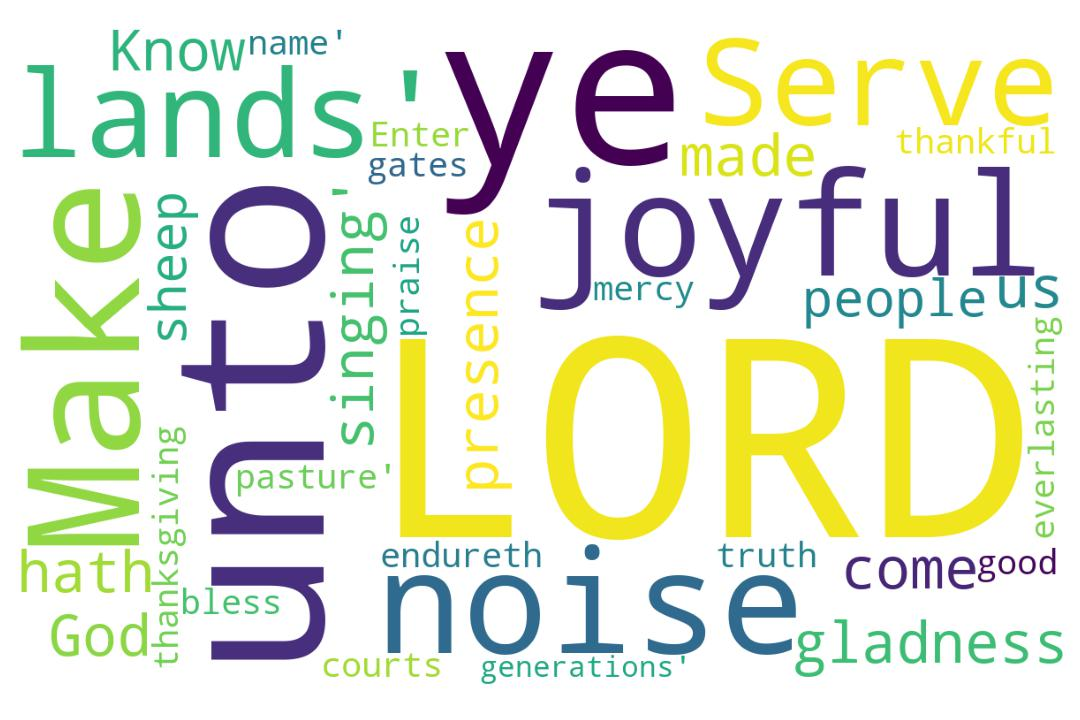
\includegraphics[width=\linewidth]{19OT-Psalms/Psalm100-WordCloud.jpg}
  \caption{Psalm 100 Word Cloud}
  \label{fig:Psalm 100 word Cloud}
\end{figure}


\marginpar{\scriptsize \centering \fcolorbox{bone}{lime}{\textbf{BECAUSE GOD IS GOOD}}\\ (Psalm 100:1-5)

\begin{compactenum}[I.][8]
    \item The \textbf{Geography} of Praise \index[scripture]{Psalms!Psa 100:01} (Psa 100:1)
    \item The \textbf{Gladness} of Praise \index[scripture]{Psalms!Psa 100:02} (Psa 100:2)
    \item Like \textbf{Grazing} Sheep \index[scripture]{Psalms!Psa 100:03} (Psa 100:3)
    \item The \textbf{Gates} of Thanksgiving \index[scripture]{Psalms!Psa 100:04} (Psa 100:4)
    \item The \textbf{Gladness} \index[scripture]{Psalms!Psa 100:02} (Psa 100:2)
    \item The \textbf{Gratitude} \index[scripture]{Psalms!Psa 100:02} (Psa 100:2)
    \item All \textbf{Generations} \index[scripture]{Psalms!Psa 100:05} (Psa 100:5)
    \item Because He is \textbf{Good} \index[scripture]{Psalms!Psa 100:05} (Psa 100:5)
\end{compactenum}}




\footnote{\textcolor[rgb]{0.00,0.25,0.00}{\hyperlink{TOC}{Return to end of Table of Contents.}}}\footnote{\href{https://audiobible.com/bible/psalms_100.html}{\textcolor[cmyk]{0.99998,1,0,0}{Psalm 100 Audio}}}\textcolor[cmyk]{0.99998,1,0,0}{A Psalm of praise.}\\
\\
\textcolor[cmyk]{0.99998,1,0,0}{Make a joyful noise unto the LORD, \fcolorbox{bone}{lime}{all ye lands}.}
[2] \textcolor[cmyk]{0.99998,1,0,0}{Serve the LORD with \fcolorbox{bone}{lime}{gladness}: come before his presence with singing.}
[3] \textcolor[cmyk]{0.99998,1,0,0}{Know ye that the LORD he \emph{is} God: \emph{it} \emph{is} he \emph{that} hath made us, and not we ourselves; \emph{we} \emph{are} his people, and the \fcolorbox{bone}{lime}{sheep of his pasture}.}
[4] \textcolor[cmyk]{0.99998,1,0,0}{Enter into his \fcolorbox{bone}{lime}{gates with thanksgiving}, \emph{and} into his courts with praise: be thankful unto him, \emph{and} bless his name.}
[5] \textcolor[cmyk]{0.99998,1,0,0}{For the LORD \emph{is} \fcolorbox{bone}{lime}{good}; his mercy \emph{is} everlasting; and his truth \emph{endureth} to all \fcolorbox{bone}{lime}{generations}.}
\section{Psalm1 0 Comments}




%\index[NWIV]{10!Psalm!Psa 100:1}\index[AWIP]{Make!Psalm!Psa 100:1}\index[AWIP]{a!Psalm!Psa 100:1}\index[AWIP]{joyful!Psalm!Psa 100:1}\index[AWIP]{noise!Psalm!Psa 100:1}\index[AWIP]{unto!Psalm!Psa 100:1}\index[AWIP]{the!Psalm!Psa 100:1}\index[AWIP]{LORD!Psalm!Psa 100:1}\index[AWIP]{all!Psalm!Psa 100:1}\index[AWIP]{ye!Psalm!Psa 100:1}\index[AWIP]{lands!Psalm!Psa 100:1}

\index[NWIV]{11!Psalm!Psa 100:2}\index[AWIP]{Serve!Psalm!Psa 100:2}\index[AWIP]{the!Psalm!Psa 100:2}\index[AWIP]{LORD!Psalm!Psa 100:2}\index[AWIP]{with!Psalm!Psa 100:2}\index[AWIP]{with!Psalm!Psa 100:2 (2)}\index[AWIP]{gladness!Psalm!Psa 100:2}\index[AWIP]{come!Psalm!Psa 100:2}\index[AWIP]{before!Psalm!Psa 100:2}\index[AWIP]{his!Psalm!Psa 100:2}\index[AWIP]{presence!Psalm!Psa 100:2}\index[AWIP]{singing!Psalm!Psa 100:2}

\index[NWIV]{29!Psalm!Psa 100:3}\index[AWIP]{Know!Psalm!Psa 100:3}\index[AWIP]{ye!Psalm!Psa 100:3}\index[AWIP]{that!Psalm!Psa 100:3}\index[AWIP]{the!Psalm!Psa 100:3}\index[AWIP]{the!Psalm!Psa 100:3 (2)}\index[AWIP]{LORD!Psalm!Psa 100:3}\index[AWIP]{he!Psalm!Psa 100:3}\index[AWIP]{he!Psalm!Psa 100:3 (2)}\index[AWIP]{\emph{is}!Psalm!Psa 100:3}\index[AWIP]{\emph{is}!Psalm!Psa 100:3 (2)}\index[AWIP]{God!Psalm!Psa 100:3}\index[AWIP]{\emph{it}!Psalm!Psa 100:3}\index[AWIP]{\emph{that}!Psalm!Psa 100:3}\index[AWIP]{hath!Psalm!Psa 100:3}\index[AWIP]{made!Psalm!Psa 100:3}\index[AWIP]{us!Psalm!Psa 100:3}\index[AWIP]{and!Psalm!Psa 100:3}\index[AWIP]{and!Psalm!Psa 100:3 (2)}\index[AWIP]{not!Psalm!Psa 100:3}\index[AWIP]{we!Psalm!Psa 100:3}\index[AWIP]{ourselves!Psalm!Psa 100:3}\index[AWIP]{\emph{we}!Psalm!Psa 100:3}\index[AWIP]{\emph{are}!Psalm!Psa 100:3}\index[AWIP]{his!Psalm!Psa 100:3}\index[AWIP]{his!Psalm!Psa 100:3 (2)}\index[AWIP]{people!Psalm!Psa 100:3}\index[AWIP]{sheep!Psalm!Psa 100:3}\index[AWIP]{of!Psalm!Psa 100:3}\index[AWIP]{pasture!Psalm!Psa 100:3}\index[AWIP]{\emph{is}!Psalm!Psa 100:3}\index[AWIP]{\emph{is}!Psalm!Psa 100:3 (2)}\index[AWIP]{\emph{it}!Psalm!Psa 100:3}\index[AWIP]{\emph{that}!Psalm!Psa 100:3}\index[AWIP]{\emph{we}!Psalm!Psa 100:3}\index[AWIP]{\emph{are}!Psalm!Psa 100:3}

\index[NWIV]{20!Psalm!Psa 100:4}\index[AWIP]{Enter!Psalm!Psa 100:4}\index[AWIP]{into!Psalm!Psa 100:4}\index[AWIP]{into!Psalm!Psa 100:4 (2)}\index[AWIP]{his!Psalm!Psa 100:4}\index[AWIP]{his!Psalm!Psa 100:4 (2)}\index[AWIP]{his!Psalm!Psa 100:4 (3)}\index[AWIP]{gates!Psalm!Psa 100:4}\index[AWIP]{with!Psalm!Psa 100:4}\index[AWIP]{with!Psalm!Psa 100:4 (2)}\index[AWIP]{thanksgiving!Psalm!Psa 100:4}\index[AWIP]{\emph{and}!Psalm!Psa 100:4}\index[AWIP]{\emph{and}!Psalm!Psa 100:4 (2)}\index[AWIP]{courts!Psalm!Psa 100:4}\index[AWIP]{praise!Psalm!Psa 100:4}\index[AWIP]{be!Psalm!Psa 100:4}\index[AWIP]{thankful!Psalm!Psa 100:4}\index[AWIP]{unto!Psalm!Psa 100:4}\index[AWIP]{him!Psalm!Psa 100:4}\index[AWIP]{bless!Psalm!Psa 100:4}\index[AWIP]{name!Psalm!Psa 100:4}\index[AWIP]{\emph{and}!Psalm!Psa 100:4}\index[AWIP]{\emph{and}!Psalm!Psa 100:4 (2)}

\index[NWIV]{16!Psalm!Psa 100:5}\index[AWIP]{For!Psalm!Psa 100:5}\index[AWIP]{the!Psalm!Psa 100:5}\index[AWIP]{LORD!Psalm!Psa 100:5}\index[AWIP]{\emph{is}!Psalm!Psa 100:5}\index[AWIP]{\emph{is}!Psalm!Psa 100:5 (2)}\index[AWIP]{good!Psalm!Psa 100:5}\index[AWIP]{his!Psalm!Psa 100:5}\index[AWIP]{his!Psalm!Psa 100:5 (2)}\index[AWIP]{mercy!Psalm!Psa 100:5}\index[AWIP]{everlasting!Psalm!Psa 100:5}\index[AWIP]{and!Psalm!Psa 100:5}\index[AWIP]{truth!Psalm!Psa 100:5}\index[AWIP]{\emph{endureth}!Psalm!Psa 100:5}\index[AWIP]{to!Psalm!Psa 100:5}\index[AWIP]{all!Psalm!Psa 100:5}\index[AWIP]{generations!Psalm!Psa 100:5}\index[AWIP]{\emph{is}!Psalm!Psa 100:5}\index[AWIP]{\emph{is}!Psalm!Psa 100:5 (2)}\index[AWIP]{\emph{endureth}!Psalm!Psa 100:5}


\section{Psalm 100 Outlines}

\subsection{My Outlines}

\subsubsection{Because God is Good}

\index[speaker]{Keith Anthony!Psalm 100 (Because God is Good)}
\index[series]{Psalms (Keith Anthony)!Psalm 100 (Because God is Good)}
\index[date]{2017/09/02!Psalm 100 (Because God is Good) (Keith Anthony)}

\begin{compactenum}[I.]
    \item The \textbf{Geography} of Praise \index[scripture]{Psalms!Psa 100:01} (Psa 100:1)
    \item The \textbf{Gladness} of Praise \index[scripture]{Psalms!Psa 100:02} (Psa 100:2)
    \item Like \textbf{Grazing} Sheep \index[scripture]{Psalms!Psa 100:03} (Psa 100:3)
    \item The \textbf{Gates} of Thanksgiving \index[scripture]{Psalms!Psa 100:04} (Psa 100:4)
    \item The \textbf{Gratitude} \index[scripture]{Psalms!Psa 100:02} (Psa 100:2)
    \item All \textbf{Generations} \index[scripture]{Psalms!Psa 100:05} (Psa 100:5)
    \item Because He is \textbf{Good} \index[scripture]{Psalms!Psa 100:05} (Psa 100:5)
\end{compactenum}


\subsection{Outlines from Others}


%\section{Psalm 100 Statistics}

%%%%%%%%%%%%%%%%%%%%%%%%%%%
%%%%% Word Statistics
%%%%%%%%%%%%%%%%%%%%%%%%%%


\normalsize



\subsection{Chapter Word Statistics}


%%%%%%%%%%
%%%%%%%%%%
 
\begin{center}
\begin{longtable}{l|c|c|c|c}
\caption[Stats for Psalm 100]{Stats for Psalm 100} \label{table:Stats for Psalm 100} \\ 
\hline \multicolumn{1}{|c|}{\textbf{Verse(s)}} & \multicolumn{1}{|c|}{\textbf{Count}} & \multicolumn{1}{|c|}{\textbf{Unique}} & \multicolumn{1}{|c|}{\textbf{Italics}} & \multicolumn{1}{|c|}{\textbf{Uniq Italic}}  \\ \hline 
\endfirsthead
 
\multicolumn{5}{c}
{{\bfseries \tablename\ \thetable{} -- continued from previous page}} \\  
\hline \multicolumn{1}{|c|}{\textbf{Verse(s)}} & \multicolumn{1}{|c|}{\textbf{Count}} & \multicolumn{1}{|c|}{\textbf{Unique}} & \multicolumn{1}{|c|}{\textbf{Italics}} & \multicolumn{1}{|c|}{\textbf{Uniq Italic}}  \\ \hline 
\endhead
 
\hline \multicolumn{5}{|r|}{{Continued if needed}} \\ \hline
\endfoot 
1 & 10 & 10 & 0 & 0\\ \hline
2 & 11 & 10 & 0 & 0\\ \hline
3 & 29 & 24 & 6 & 5\\ \hline
4 & 20 & 15 & 2 & 1\\ \hline
5 & 16 & 14 & 3 & 2\\ \hline
\hline \hline
Total & 86 & 58 & 11 & 7



\end{longtable}
\end{center}

%%%%%%%%%%
%%%%%%%%%%
 
\subsection{Words by Frequency}
\scriptsize
\begin{center}
\begin{longtable}{l|r}
\caption[Word Frequencies in Psalm 100]{Word Frequencies in Psalm 100} \label{table:WordsIn-Psalm-100} \\ 
\hline \multicolumn{1}{|c|}{\textbf{Word}} & \multicolumn{1}{c|}{\textbf{Frequency}} \\ \hline 
\endfirsthead
 
\multicolumn{2}{c}
{{\bfseries \tablename\ \thetable{} -- continued from previous page}} \\ 
\hline \multicolumn{1}{|c|}{\textbf{Word}} & \multicolumn{1}{c|}{\textbf{Frequency}} \\ \hline 
\endhead
 
\hline \multicolumn{2}{|r|}{{Continued if needed}} \\ \hline
\endfoot
 
\hline \hline
\endlastfoot
his & 8 \\ \hline
the & 5 \\ \hline
LORD & 4 \\ \hline
with & 4 \\ \hline
\emph{is} & 4 \\ \hline
and & 3 \\ \hline
unto & 2 \\ \hline
all & 2 \\ \hline
ye & 2 \\ \hline
he & 2 \\ \hline
into & 2 \\ \hline
\emph{and} & 2 \\ \hline
Make & 1 \\ \hline
a & 1 \\ \hline
joyful & 1 \\ \hline
noise & 1 \\ \hline
lands & 1 \\ \hline
Serve & 1 \\ \hline
gladness & 1 \\ \hline
come & 1 \\ \hline
before & 1 \\ \hline
presence & 1 \\ \hline
singing & 1 \\ \hline
Know & 1 \\ \hline
that & 1 \\ \hline
God & 1 \\ \hline
\emph{it} & 1 \\ \hline
\emph{that} & 1 \\ \hline
hath & 1 \\ \hline
made & 1 \\ \hline
us & 1 \\ \hline
not & 1 \\ \hline
we & 1 \\ \hline
ourselves & 1 \\ \hline
\emph{we} & 1 \\ \hline
\emph{are} & 1 \\ \hline
people & 1 \\ \hline
sheep & 1 \\ \hline
of & 1 \\ \hline
pasture & 1 \\ \hline
Enter & 1 \\ \hline
gates & 1 \\ \hline
thanksgiving & 1 \\ \hline
courts & 1 \\ \hline
praise & 1 \\ \hline
be & 1 \\ \hline
thankful & 1 \\ \hline
him & 1 \\ \hline
bless & 1 \\ \hline
name & 1 \\ \hline
For & 1 \\ \hline
good & 1 \\ \hline
mercy & 1 \\ \hline
everlasting & 1 \\ \hline
truth & 1 \\ \hline
\emph{endureth} & 1 \\ \hline
to & 1 \\ \hline
generations & 1 \\ \hline
\end{longtable}
\end{center}



\normalsize



\subsection{Words Alphabetically}
\scriptsize
\begin{center}
\begin{longtable}{l|r}
\caption[Word Alphabetically in Psalm 100]{Word Alphabetically in Psalm 100} \label{table:WordsIn-Psalm-100} \\ 
\hline \multicolumn{1}{|c|}{\textbf{Word}} & \multicolumn{1}{c|}{\textbf{Frequency}} \\ \hline 
\endfirsthead
 
\multicolumn{2}{c}
{{\bfseries \tablename\ \thetable{} -- continued from previous page}} \\ 
\hline \multicolumn{1}{|c|}{\textbf{Word}} & \multicolumn{1}{c|}{\textbf{Frequency}} \\ \hline 
\endhead
 
\hline \multicolumn{2}{|r|}{{Continued if needed}} \\ \hline
\endfoot
 
\hline \hline
\endlastfoot
Enter & 1 \\ \hline
For & 1 \\ \hline
God & 1 \\ \hline
Know & 1 \\ \hline
LORD & 4 \\ \hline
Make & 1 \\ \hline
Serve & 1 \\ \hline
\emph{and} & 2 \\ \hline
\emph{are} & 1 \\ \hline
\emph{endureth} & 1 \\ \hline
\emph{is} & 4 \\ \hline
\emph{it} & 1 \\ \hline
\emph{that} & 1 \\ \hline
\emph{we} & 1 \\ \hline
a & 1 \\ \hline
all & 2 \\ \hline
and & 3 \\ \hline
be & 1 \\ \hline
before & 1 \\ \hline
bless & 1 \\ \hline
come & 1 \\ \hline
courts & 1 \\ \hline
everlasting & 1 \\ \hline
gates & 1 \\ \hline
generations & 1 \\ \hline
gladness & 1 \\ \hline
good & 1 \\ \hline
hath & 1 \\ \hline
he & 2 \\ \hline
him & 1 \\ \hline
his & 8 \\ \hline
into & 2 \\ \hline
joyful & 1 \\ \hline
lands & 1 \\ \hline
made & 1 \\ \hline
mercy & 1 \\ \hline
name & 1 \\ \hline
noise & 1 \\ \hline
not & 1 \\ \hline
of & 1 \\ \hline
ourselves & 1 \\ \hline
pasture & 1 \\ \hline
people & 1 \\ \hline
praise & 1 \\ \hline
presence & 1 \\ \hline
sheep & 1 \\ \hline
singing & 1 \\ \hline
thankful & 1 \\ \hline
thanksgiving & 1 \\ \hline
that & 1 \\ \hline
the & 5 \\ \hline
to & 1 \\ \hline
truth & 1 \\ \hline
unto & 2 \\ \hline
us & 1 \\ \hline
we & 1 \\ \hline
with & 4 \\ \hline
ye & 2 \\ \hline
\end{longtable}
\end{center}



\normalsize



\subsection{Word Lengths in Chapter}
\normalsize
\begin{longtable}{l|p{3.75in}}
\caption[Words by Length in Psalm 100]{Words by Length in Psalm 100} \label{table:WordsIn-Psalm-100} \\ 
\hline \multicolumn{1}{|c|}{\textbf{Length}} & \multicolumn{1}{c|}{\textbf{Words}} \\ \hline 
\endfirsthead
 
\multicolumn{2}{c}
{{\bfseries \tablename\ \thetable{} -- continued from previous page}} \\ 
\hline \multicolumn{1}{|c|}{\textbf{Length}} & \multicolumn{1}{c|}{\textbf{Words}} \\ \hline 
\endhead
 
\hline \multicolumn{2}{|r|}{{Continued if needed}} \\ \hline
\endfoot
 
\hline \hline
\endlastfoot
1 & a \\ \hline
2 & ye, he, \emph{is}, \emph{it}, us, we, \emph{we}, of, be, to \\ \hline
3 & the, all, his, God, and, not, \emph{are}, \emph{and}, him, For \\ \hline
4 & Make, unto, LORD, with, come, Know, that, \emph{that}, hath, made, into, name, good \\ \hline
5 & noise, lands, Serve, sheep, Enter, gates, bless, mercy, truth \\ \hline
6 & joyful, before, people, courts, praise \\ \hline
7 & singing, pasture \\ \hline
8 & gladness, presence, thankful, \emph{endureth} \\ \hline
9 & ourselves \\ \hline
11 & everlasting, generations \\ \hline
12 & thanksgiving \\ \hline
\end{longtable}






%%%%%%%%%%
%%%%%%%%%%
\subsection{Psalm 100 Repeated Phrases}


%%%%%%%%%%
%%%%%%%%%%
\normalsize
 
\begin{center}
\begin{longtable}{|c|c|}
\caption[Psalm 100 Repeated Phrases]{Psalm 100 Repeated Phrases}\label{table:Repeated Phrases Psalm 100} \\
\hline \multicolumn{1}{|c|}{\textbf{Phrase}} & \multicolumn{1}{c|}{\textbf{Frequency}} \\ \hline 
\endfirsthead
 
\multicolumn{2}{c}
{{\bfseries \tablename\ \thetable{} -- continued from previous page}} \\  
\hline \multicolumn{1}{|c|}{\textbf{Phrase}} & \multicolumn{1}{c|}{\textbf{Frequency}} \\ \hline 
\endhead
 
\hline \multicolumn{2}{c}{{ }} \\ \hline
\endfoot 
the LORD & 4\\ \hline 
\end{longtable}
\end{center}



%%%%%%%%%%
%%%%%%%%%%






%\input{Template}
\scriptsize

\chapter{Indices}

\printindex[DOCTRINES]
\printindex[scripture]

\printindex[speaker]
%\printindex[series]

\printindex[FACEBOOK]
\printindex[LOCATION]

\printindex[AWIP]


\printbibliography
\end{document}

